% Mirror: https://github.com/SIGma-UIUC/presentation-format
% --------------------------------------------------------------------
% This is a simple Beamer document that uses beamerthemesigma.sty
% Reading the comments should help you create a presentation even if
% you've never used Beamer before.
% --------------------------------------------------------------------

% Set our document class to Beamer
\documentclass[aspectratio=169]{beamer}

% Some packages for nice font encodings in the final PDF
\usepackage[utf8]{inputenc}
\usepackage[T1]{fontenc}

% From Jeff E
\usepackage{algo}

% Some more macros
\usepackage{sigmastyle}

% Citations
\usepackage{cite}

% To insert images
\usepackage{graphicx}

% Useful packages from the AMS
\usepackage{amsmath,amssymb,amsthm}

% Package for code highlighting
\usepackage{minted}
\setminted{linenos=true, breaklines=true, breakanywhere=true, style=default}
\usemintedstyle{monokai}

% Set a title
\title{Algorithm X}
\subtitle{\cite[Chapter~7.2.2.1]{TAOCP4B}}

% Set a subtitle if you desire
%\subtitle{\cite[Chapter~7]{TAOCP4A} and \cite[Chapter~7.2.2.1]{TAOCP4B}}

% Whoever worked on the presentation:
\author{Lou \& Anakin}

% An institute name, if you're so inclined
% \institute{University of Illinois Urbana-Champaign}

% Use the SIGma theme for this Beamer presentation
\usetheme{sigma}
% --------------------------------------------------------------------

% Begin document
\begin{document}

% Beamer calls each slide a "frame", defined within the environment:
% \begin{frame}
%   <frame content here>
% \end{frame}

% This frame is just the title.
\begin{frame}
\titlepage
\end{frame}

\date{}

% A frame with the table of contents.
% This frame's title is "Outline".
\begin{frame}{Outline}
  \tableofcontents
\end{frame}


\section{Review of Exact Cover}
\frame{\sectionpage}
\begin{frame}{Exact Cover Problems}
\begin{itemize}
    \item The goal of Exact Cover is to select subsets of some list of items according to certain criterion: \pause
    \begin{itemize}
        \item \textcolor{sigma@mainblue}{Cover:} Select subsets such that their \textbf{union} is all items
        \item \textcolor{sigma@mainblue}{Exact:} Each item is in \textbf{exactly one} subset
    \end{itemize} \pause
    \item In 1972, Richard Karp proved that Exact Cover, among 20 other problems, is \textcolor{sigma@mainblue}{NP-Complete}
        \begin{itemize}
            \item Easy to verify solutions in polynomial time
            \item Hard to solve, best known solutions run in exponential time 
            \item Can simulate (or reduce) other problems in NP using Exact Cover
        \end{itemize}
\end{itemize}
\end{frame}


\begin{frame}{An Example of Exact Cover}
    \textcolor{sigma@mainblue}{\textbf{Goal:}} Select rows such that each column in the selection has one $1$
    \[
        \begin{pmatrix}
            1 & 0 & 1 & 0 & 0  \\
            0 & 0 & 0 & 0 & 1  \\
            0 & 1 & 0 & 1 & 0  \\
            0 & 0 & 1 & 0 & 1  \\
            1 & 0 & 1 & 1 & 0  \\
        \end{pmatrix}
    \] \pause 
    We can abstract this to \textcolor{sigma@mainblue}{\underline{options}} containing \textcolor{sigma@mainblue}{\underline{items}}
    \begin{table}[]
        \begin{tabular}{ l l l }
            $1\colon \bqty{a, c}$& $2\colon \bqty{e}$ & $3\colon \bqty{b, d}$ \\ 
            $4\colon \bqty{c, e}$ & $5\colon \bqty{a, c, d}$ & \\ 
        \end{tabular}
    \end{table} \pause
    \textcolor{sigma@mainblue}{\textbf{Answer:}} Select options 1, 2, and 3
\end{frame}

\begin{frame}{Recursively Solving Exact Cover Problems}
    In trying to solve the previous problem, you may have naturally found a recursive algorithm to find a solution \pause
    \begin{nalgo}
    \underline{\textsc{FindCover}(\emph{Options, Items, Cover}, $i$)}:
    \\\label{}  \textbf{if} \emph{Cover} is a cover:\+
    \\\label{}      \textbf{terminate} successfully\-
    \\\label{}  \textbf{if} no option in \emph{Options} contains $i$:\+
    \\\label{}      \textbf{terminate} unsuccessfully\-
    \\\label{}
    \\\label{}  $I \gets$ options in \emph{Options} that contain $i$
    \\\label{}  \emph{Options} $\gets$ \emph{Options} $\setminus I$
    \\\label{}  \textbf{for} each $O$ in $I$:\+
    \\\label{}      $j \gets$ an item still not covered
    \\\label{}      \textsc{FindCover}(\emph{Options}, \emph{Cover} $\cup \set{O}$, $j$)
    \end{nalgo}
\end{frame}


\section{Data Structure}
\frame{\sectionpage}

\begin{frame}{}
    \begin{figure}
        \centering
        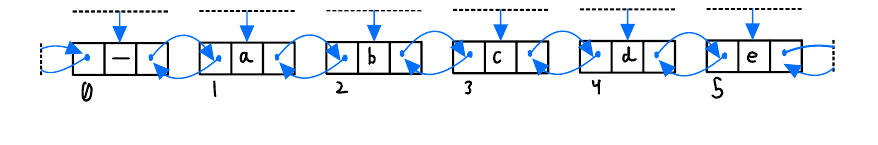
\includegraphics[scale=0.75]{images/Algorithm_X-01-cropped.png}
    \end{figure}
    \begin{itemize}
        \item We create a linked list of our \textcolor{sigma@mainblue}{\textit{items}}, where each \textcolor{sigma@mainblue}{\textit{item}} will connect to a linked list representing its \textcolor{sigma@mainblue}{\textit{options}} 
    \end{itemize}
\end{frame}

{
\usebackgroundtemplate{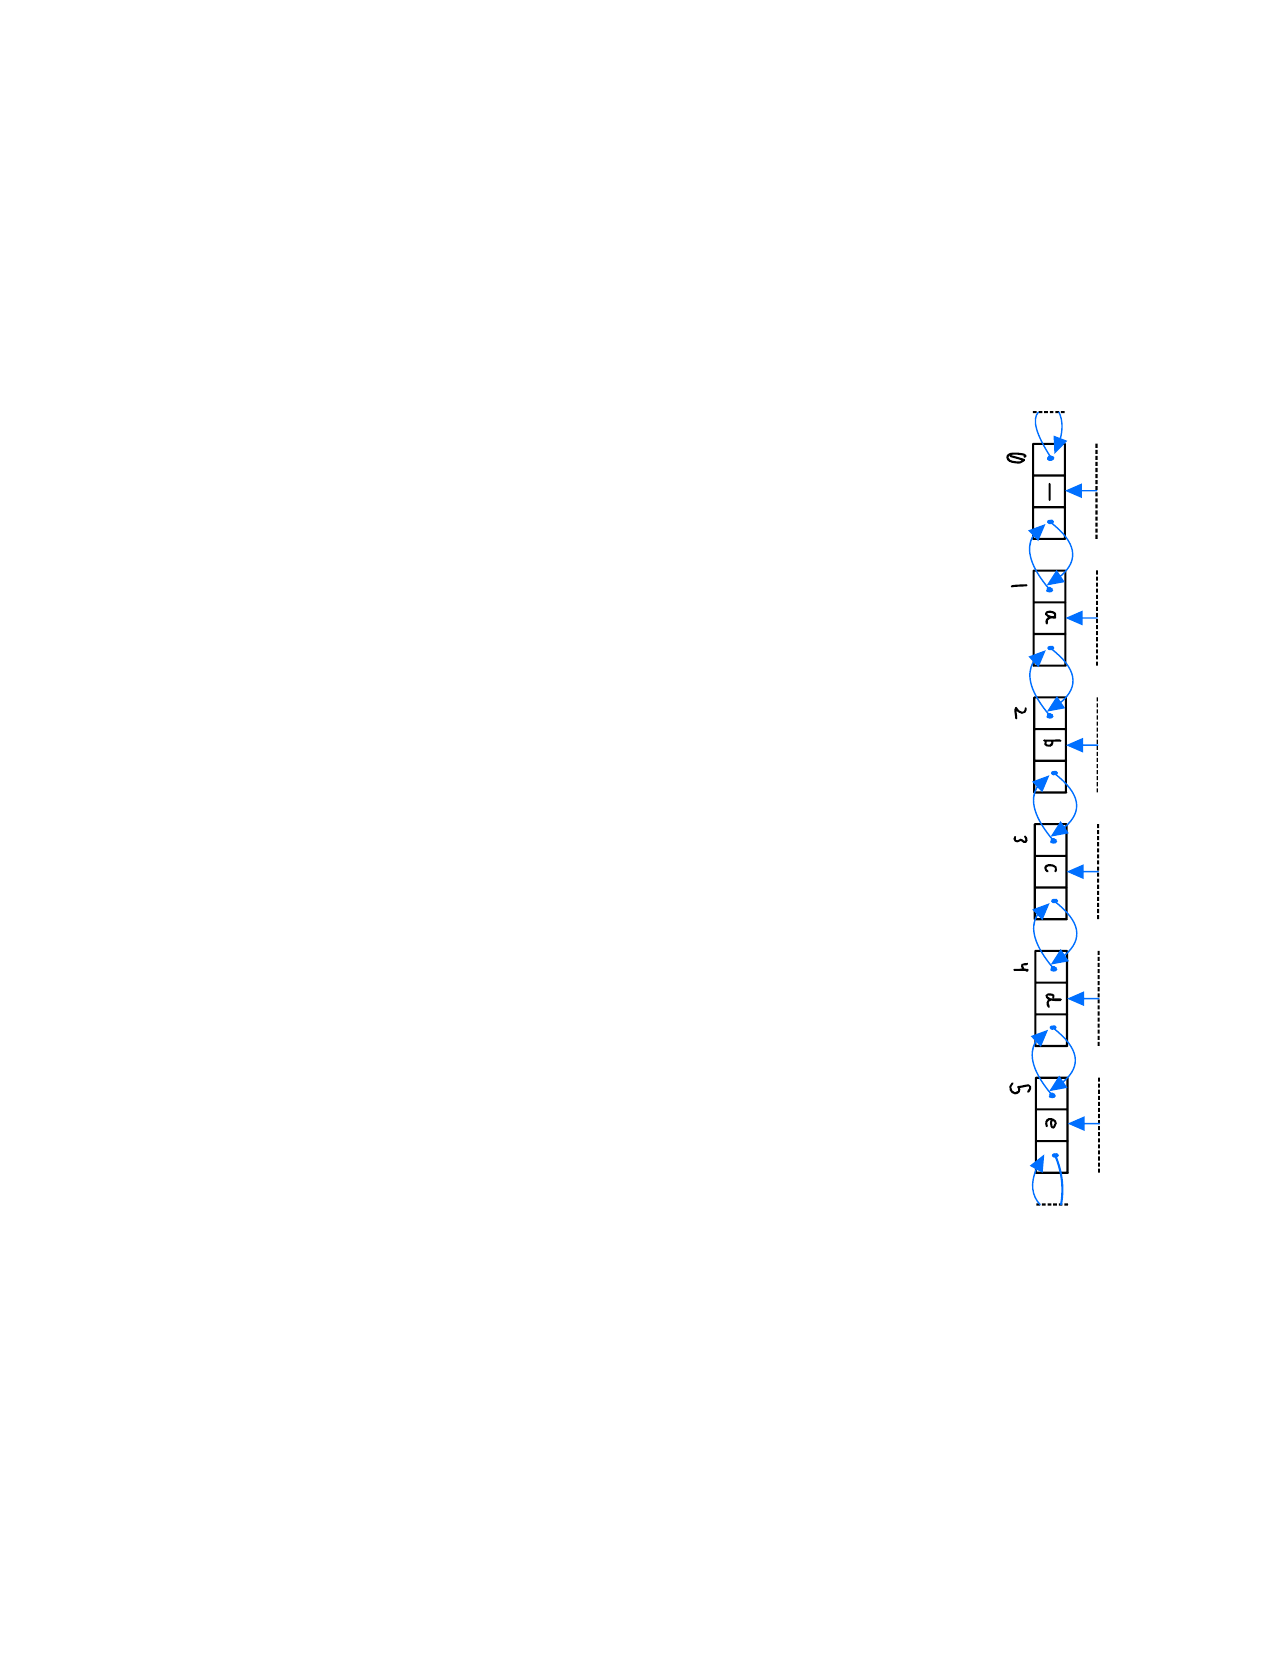
\includegraphics[angle=90,origin=c,scale=0.525]{images/Algorithm_X-01.png}}
\frame{}
}

{
\usebackgroundtemplate{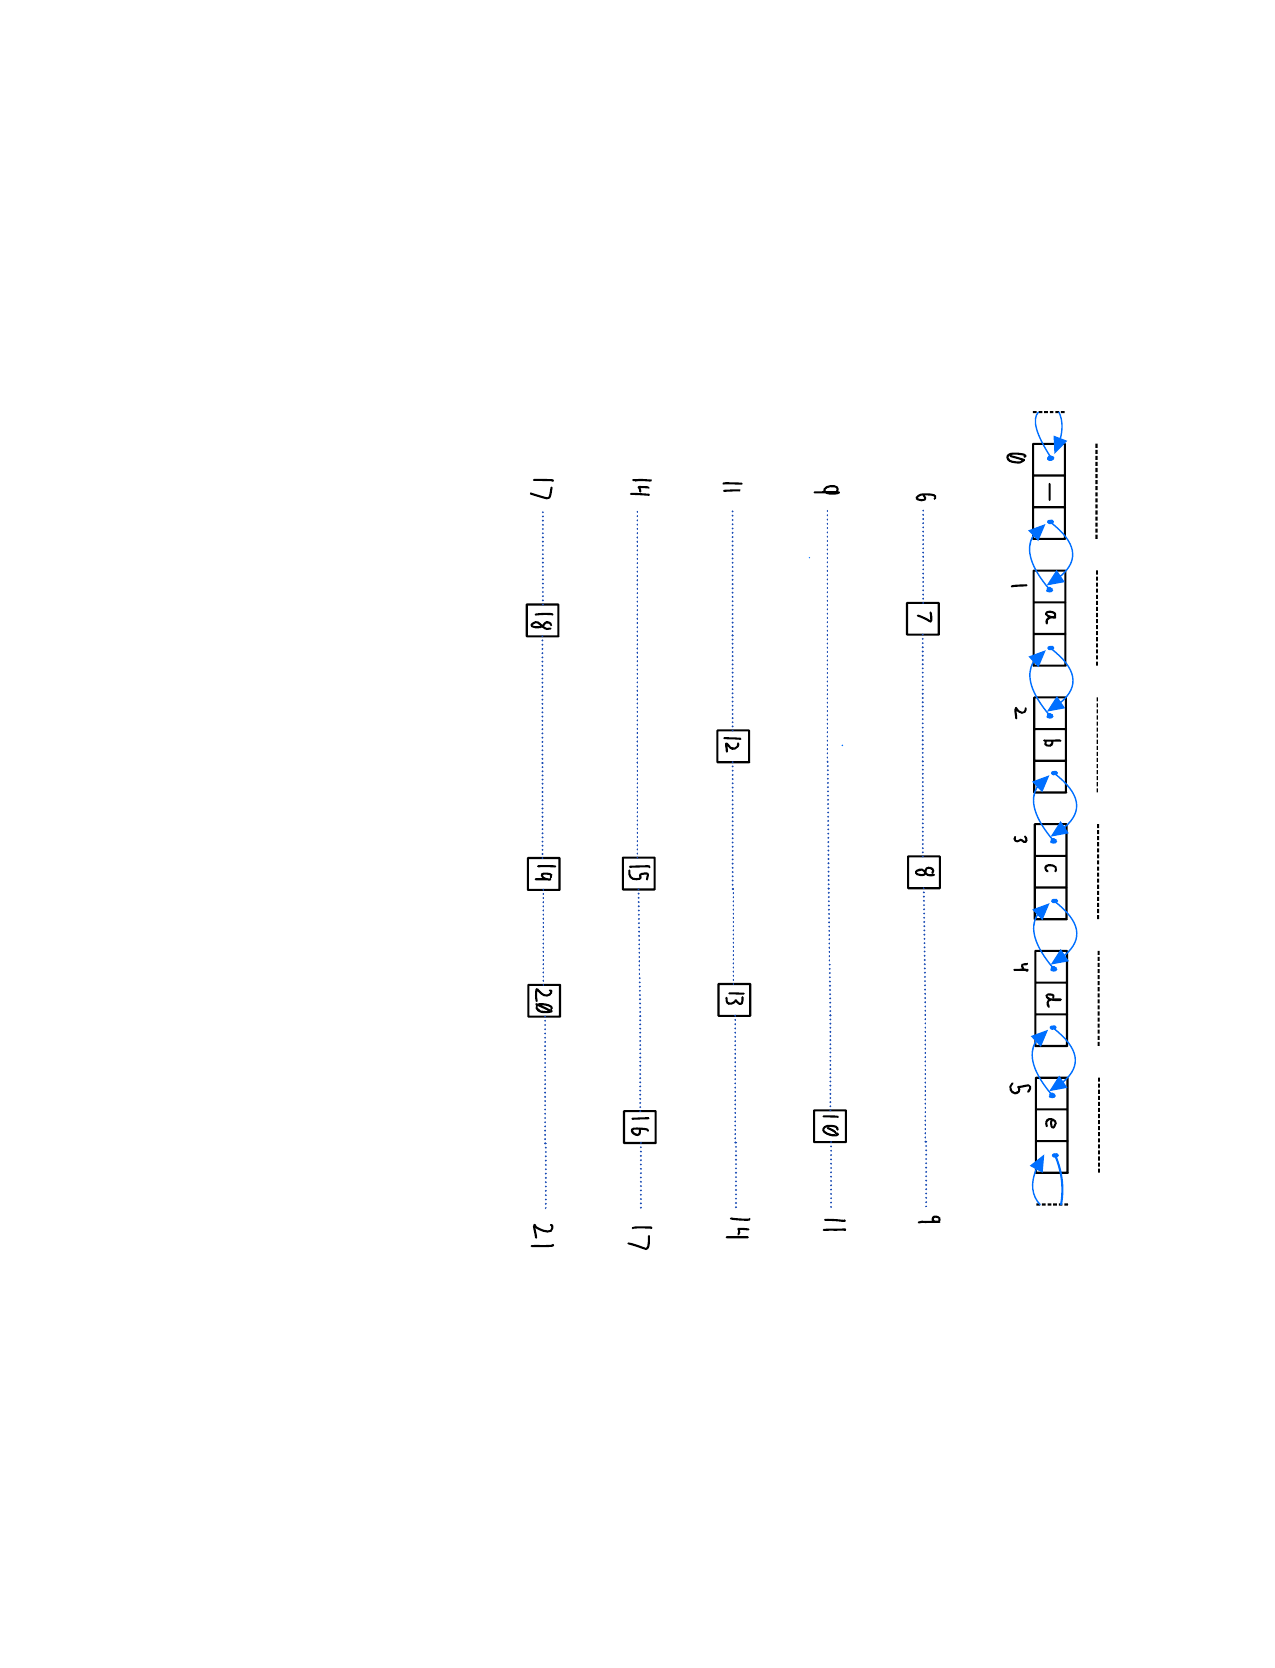
\includegraphics[angle=90,origin=c,scale=0.525]{images/Algorithm_X-02.png}}
\frame{}
}

{
\usebackgroundtemplate{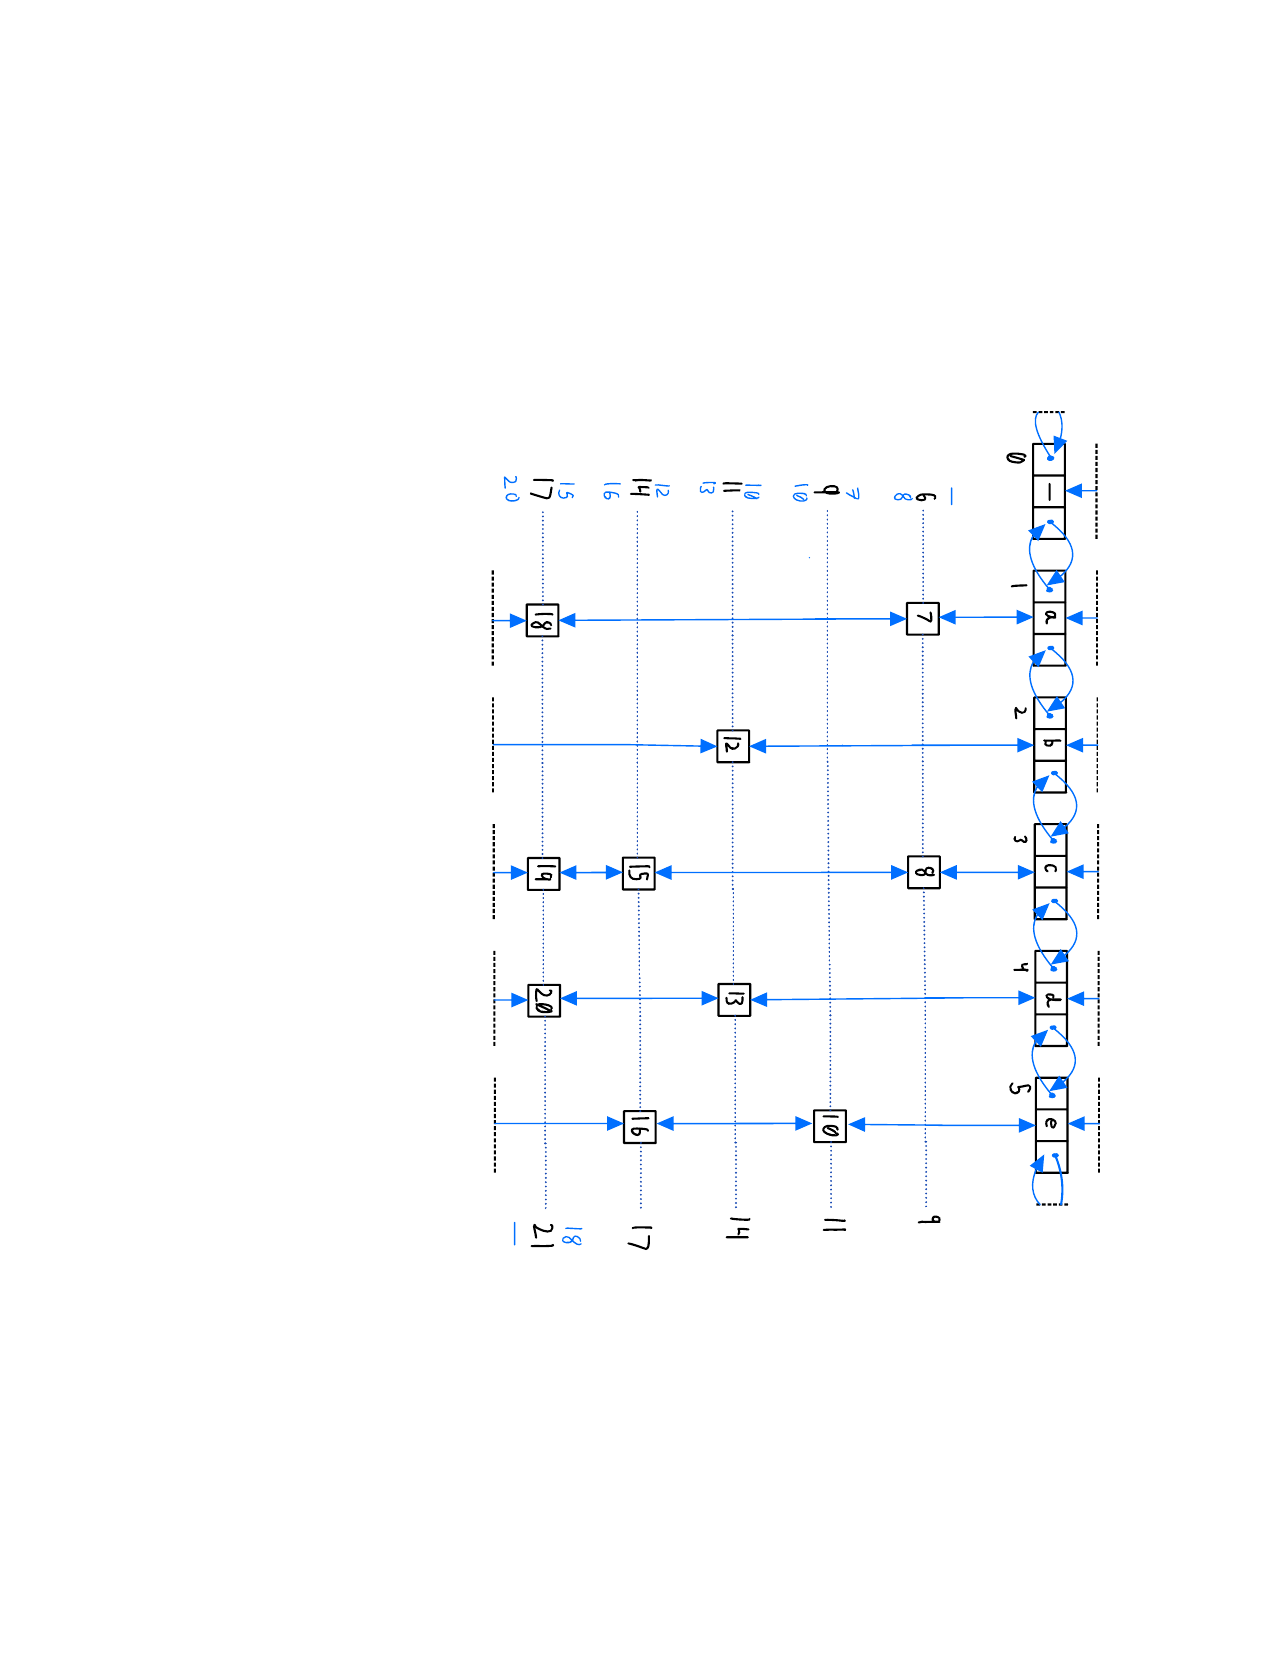
\includegraphics[angle=90,origin=c,scale=0.525]{images/Algorithm_X-03.png}}
\frame{}
}

\section{Algorithm X}
\frame{\sectionpage}

\begin{frame}{\textsc{Hide(p)}}
\begin{itemize}
    \item Removes the option a node $p$ is from (so that option can no longer be chosen)
\end{itemize}
\end{frame}

{
    \usebackgroundtemplate{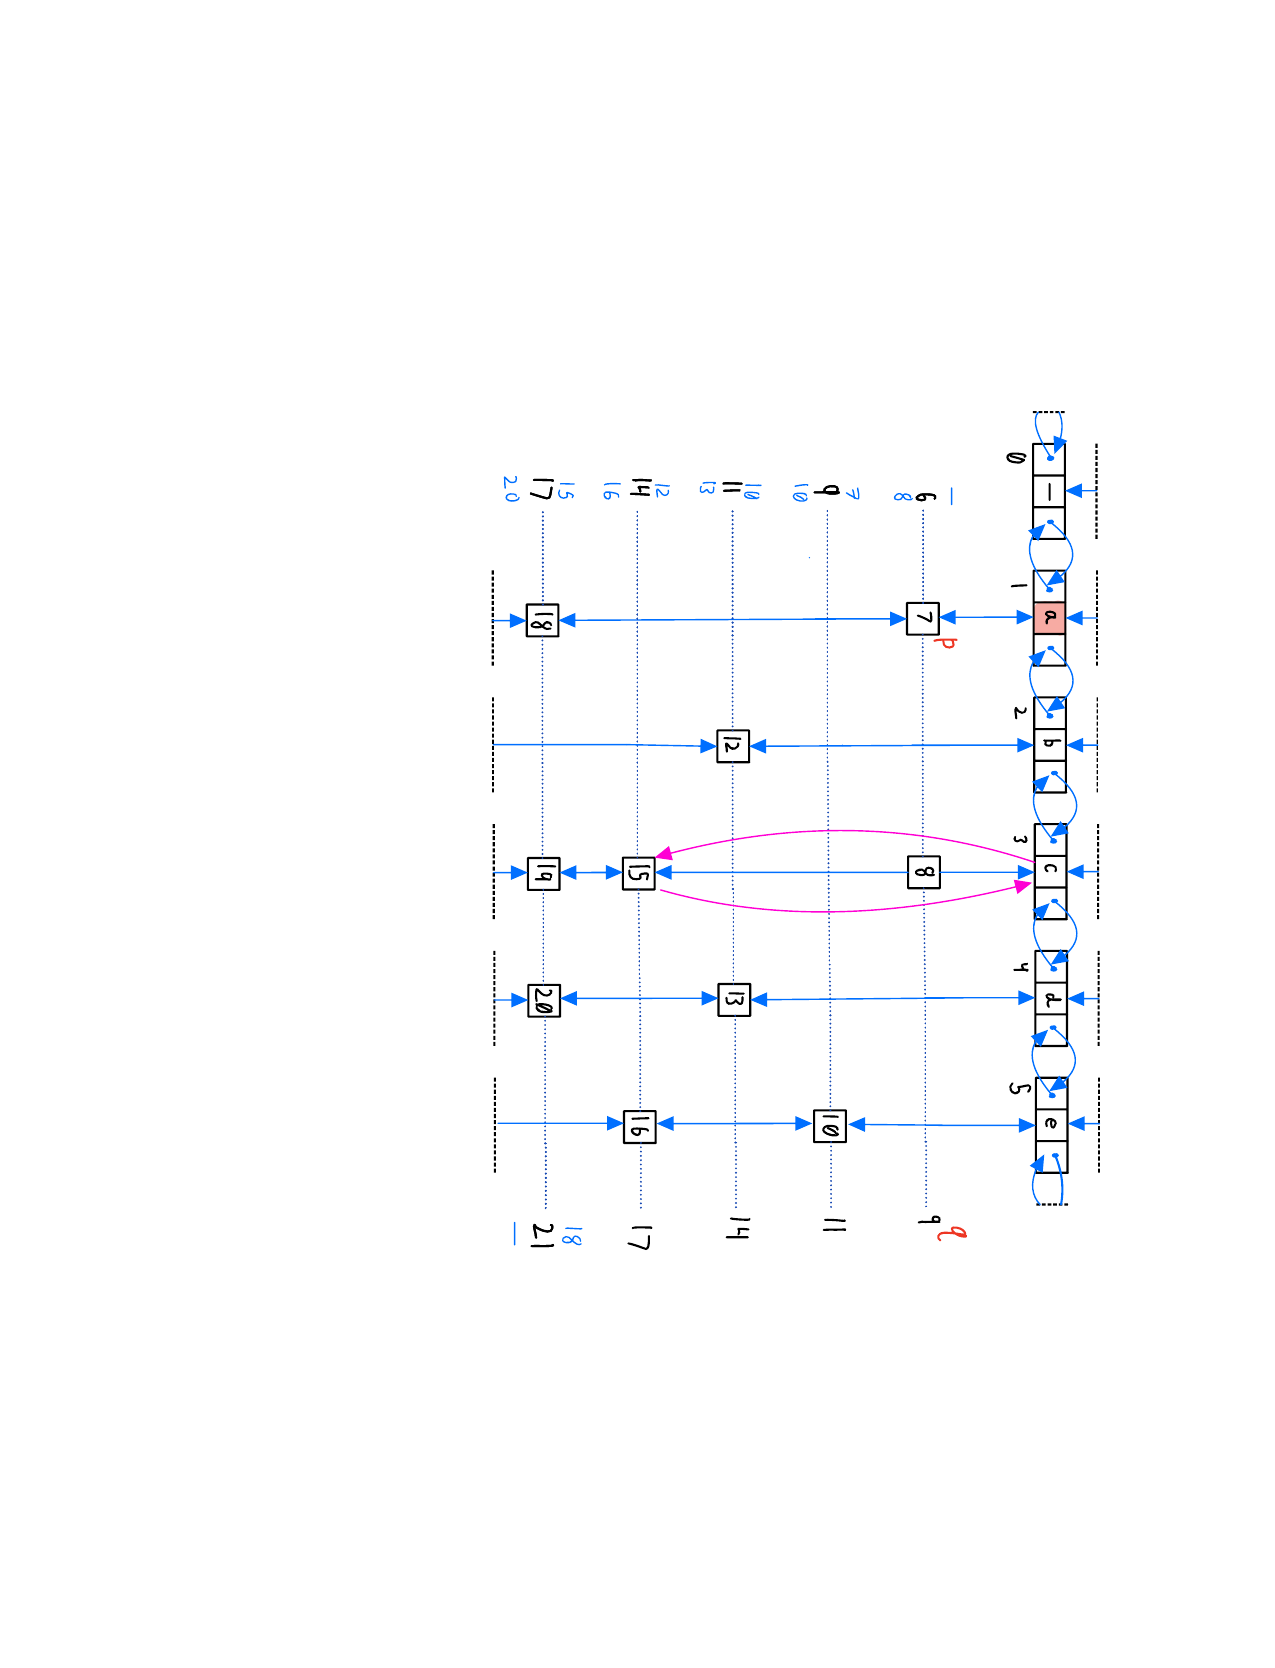
\includegraphics[angle=90,origin=c,scale=0.525]{images/Algorithm_X-07-less.png}}
    \frame{}
}


\begin{frame}{\textsc{Cover(i)}}
\begin{itemize}
    \item Hides all options that could cover item $i$
    \begin{itemize}
        \item Once we choose an option for $i$, we cannot choose any other options including $i$
    \end{itemize}
\end{itemize}
    
\end{frame}

{
    \usebackgroundtemplate{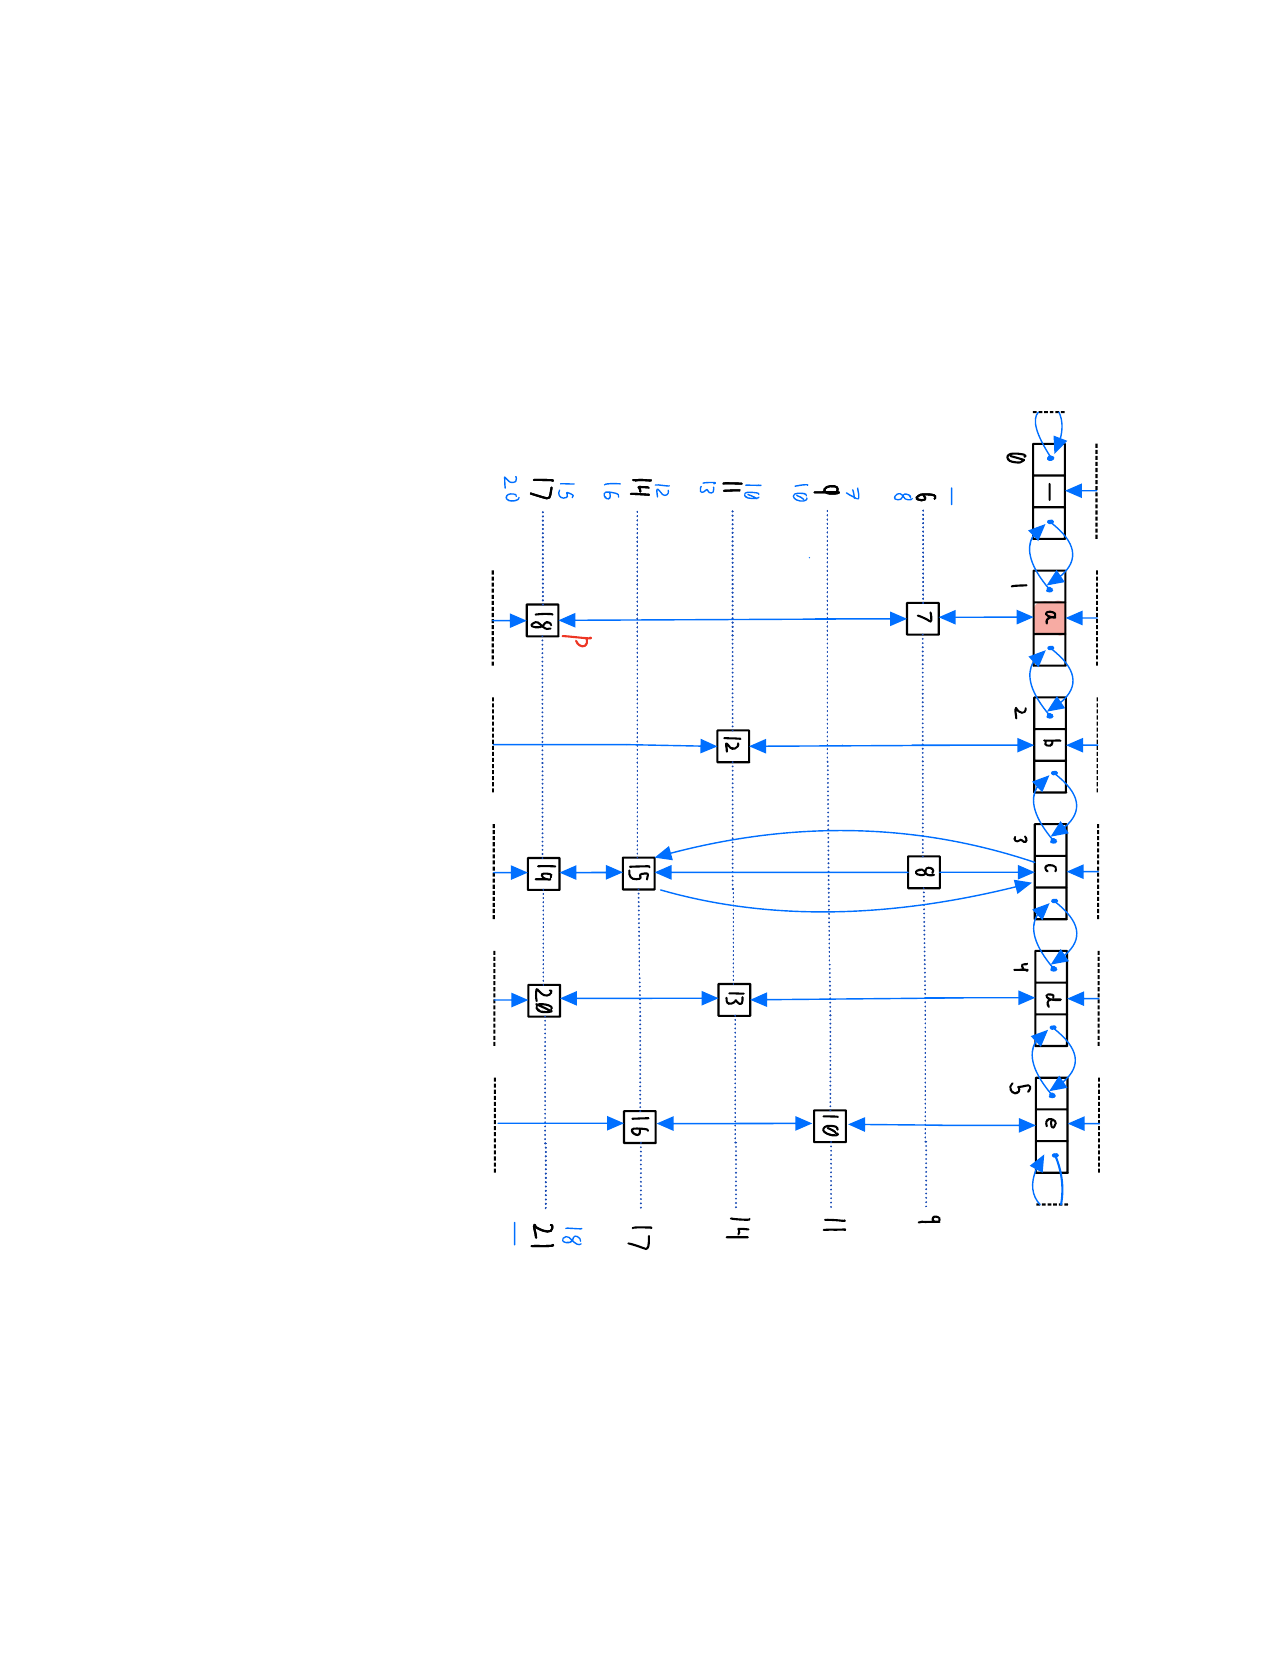
\includegraphics[angle=90,origin=c,scale=0.525]{images/Algorithm_X-09-less.png}}
    \frame{}
}

% \begin{frame}{Algorithm X}
%  \begin{itemize}
%      \item \textbf{X1:} Set up the data structure. Initialize variable $\ell=0$ (level)
%      \item \textbf{X2:} If all items have been covered, report success, recover the answer, and move to \textbf{X8.}
%      \item \textbf{X3:} If there are remaining items to be covered, choose an uncovered item $i$ to cover
%      \item \textbf{X4:} cover($i$). set $x_\ell=i.\text{down}$
%      \item \textbf{X5:} We attempt to use the option $x_\ell$ is from (let's call this option $O$) to cover $i$. 
%      \begin{itemize}
%          \item If $x_\ell=i$, then there are no remaining options to try. We backtrack (go to \textbf{X7}).
%          \item Otherwise, for each node $q$ in $O$, we call cover($q.\text{item}$) (since those items have also been covered by us selecting $O$)
%          \item set $\ell=\ell+1$. Repeat (go to \textbf{X2}).
%      \end{itemize}
%      \item \textbf{X6:} Undo the coverings from the previous step. For each node $q$ in $O$, call uncover($q.\text{item}$). Set $x_\ell=x_\ell.\text{down}$ and go to \textbf{X5}.
%      \item \textbf{X7:} uncover($i$). ($i$ could not be covered with the provided options).
%      \item\textbf{X8:} If $\ell=0$, terminate. Otherwise, set $\ell=\ell-1$ and go to \textbf{X6}.
%      
%  \end{itemize}
% \end{frame}

\begin{frame}{\textsc{Algorithm X}}
    \begin{nalgo}
    \underline{\textsc{Algorithm X}(\emph{Options, Items})}:
    \\\label{}  Set up the dancing links, $\ell \gets 0$ \Comment{$\ell$ is our level}
    \\\label{}  \textbf{if} all items have been covered:\+
    \\\label{}      Report success, visit answer, and \textbf{goto} Line 13 \-
    \\\label{}  $i \gets $ item not yet covered
    \\\label{}  \textsc{cover}($i$) then $x_\ell \gets i.$down
    \\\label{}  \textbf{if} $x_\ell = i$:\+
    \\\label{}      \textbf{goto} Line 12 \Comment{no options left to try}\-
    \\\label{}  \textbf{else}:\+
    \\\label{}      $O \gets$ option corresponding to $x_\ell$ 
    \\\label{}      \textsc{cover} every item in $O$, then \textbf{goto} Line 2\-
    \\\label{}  \textsc{uncover} items $\neq i$ in option corresponding to $x_\ell$, \textbf{goto} Line 6
    \\\label{}  \textsc{uncover}($i$)
    \\\label{}  \textbf{if} $\ell = 0$, terminate, \textbf{else} $\ell = \ell - 1$, \textbf{goto} Line 11
    \end{nalgo}
\end{frame}

{
\usebackgroundtemplate{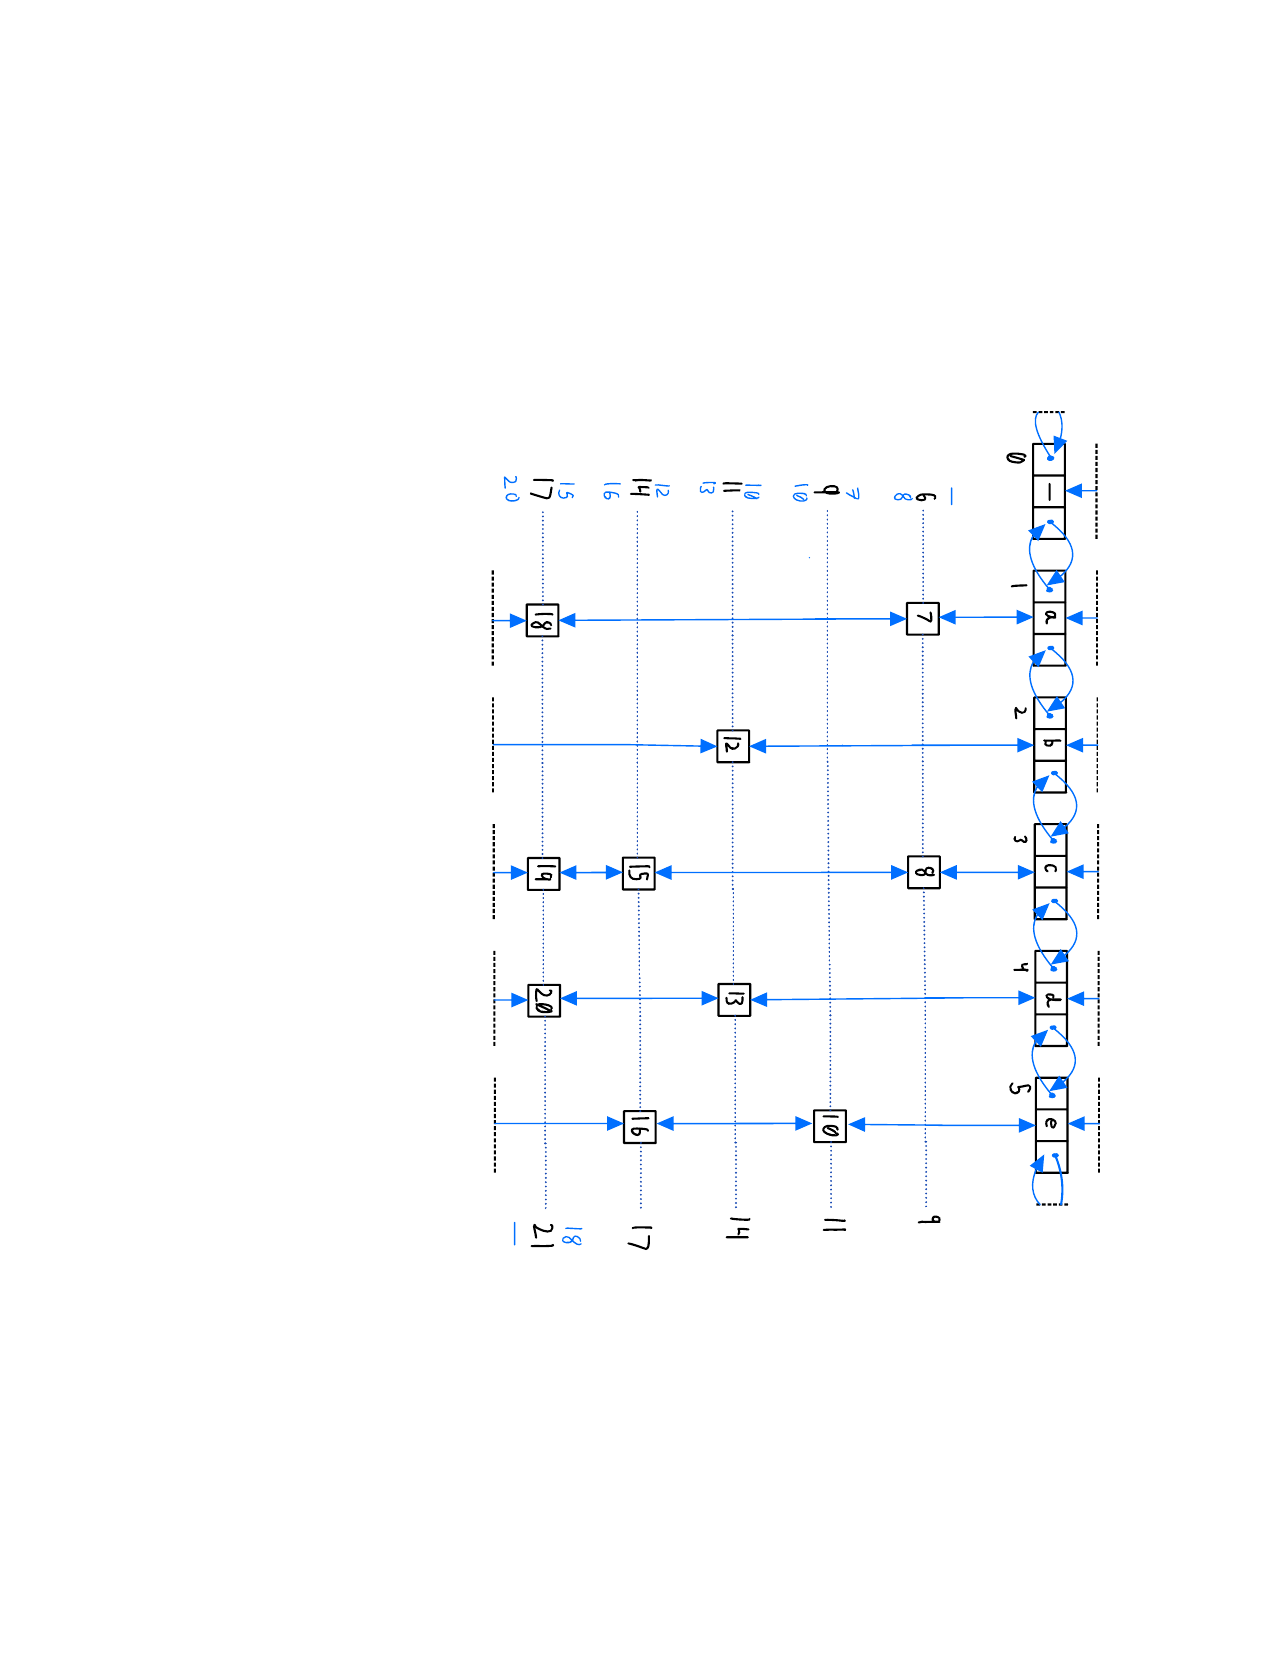
\includegraphics[angle=90,origin=c,scale=0.525]{images/Algorithm_X-03.png}}
\begin{frame}{}
    \vspace{-130pt}
    Initialize Data Structure
\end{frame} 
}

{ 
\usebackgroundtemplate{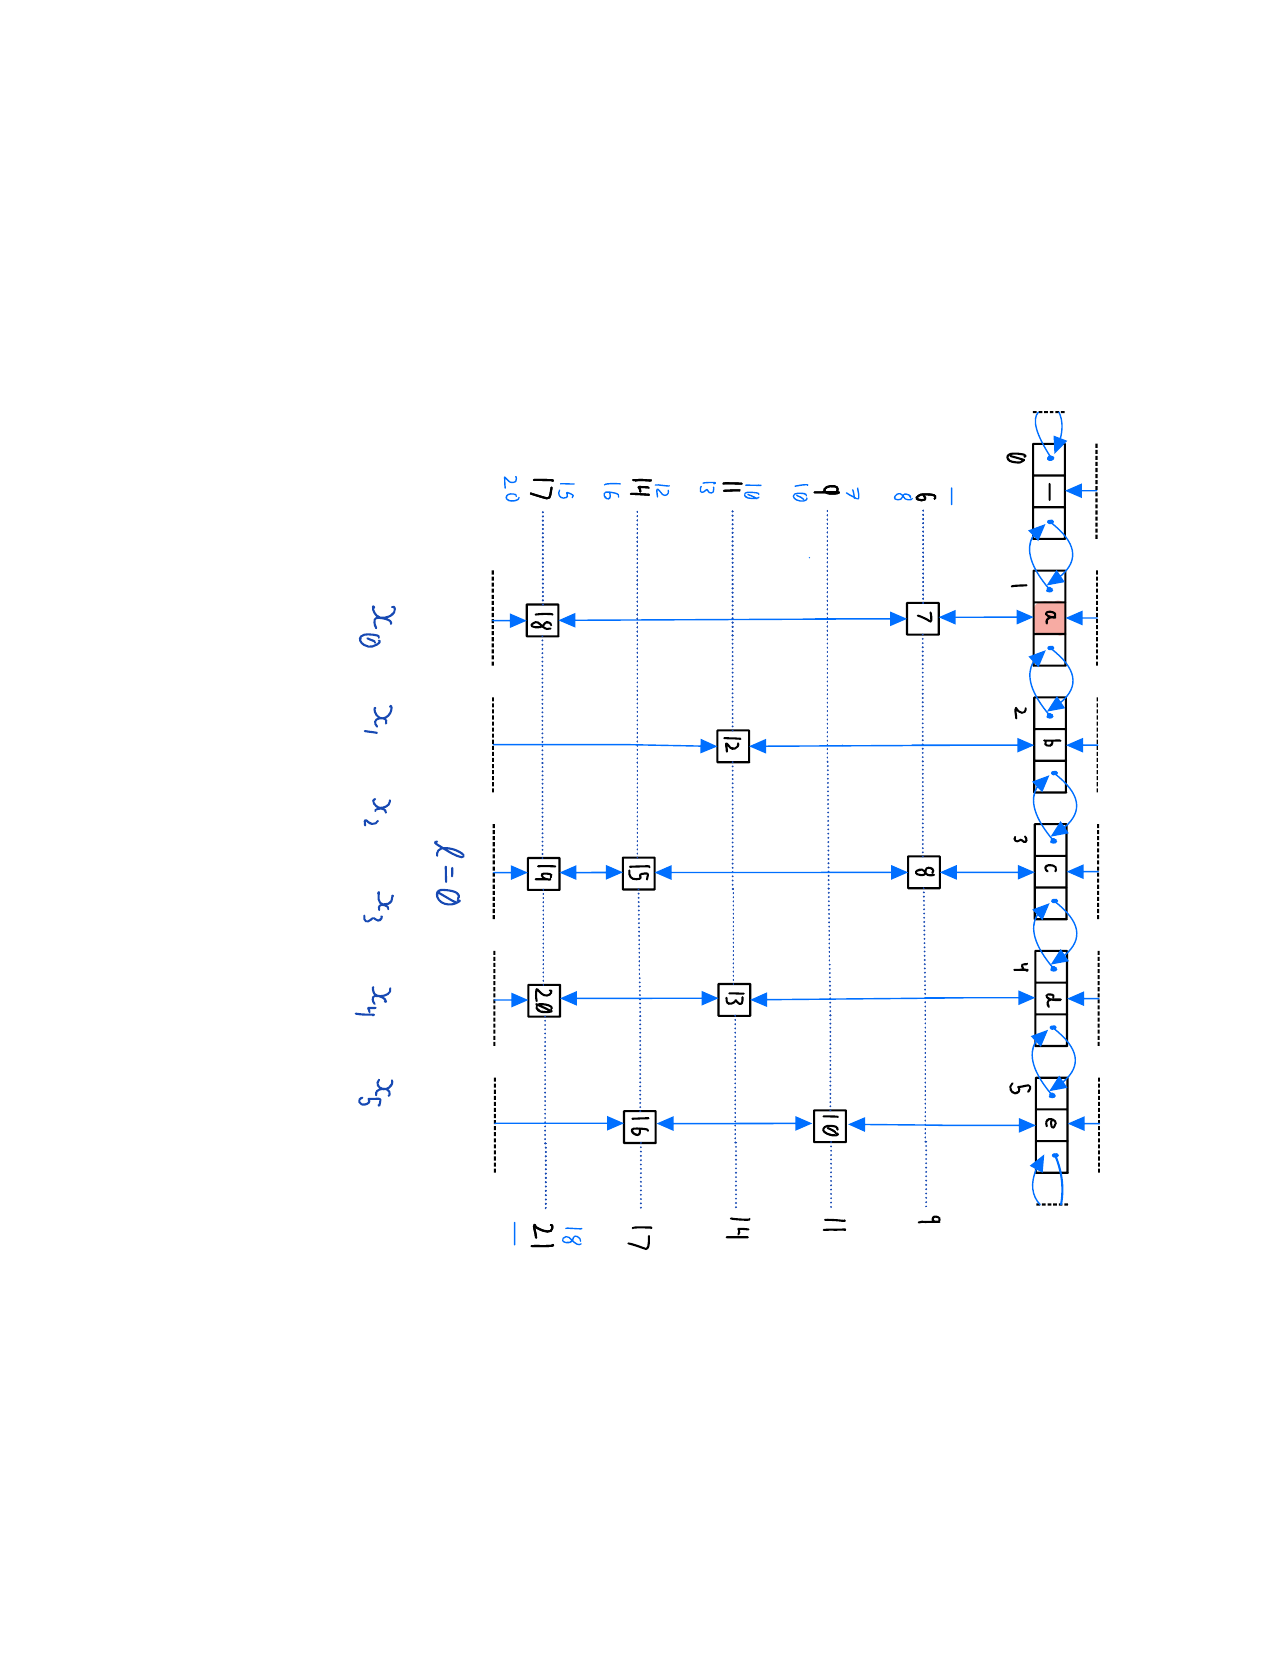
\includegraphics[angle=90,origin=c,scale=0.525]{images/Algorithm_X-04.png}} 
\begin{frame}{}
    \vspace{-130pt}
    Initialize $\ell$ and $x_\ell$'s
\end{frame} 
}

{ 
\usebackgroundtemplate{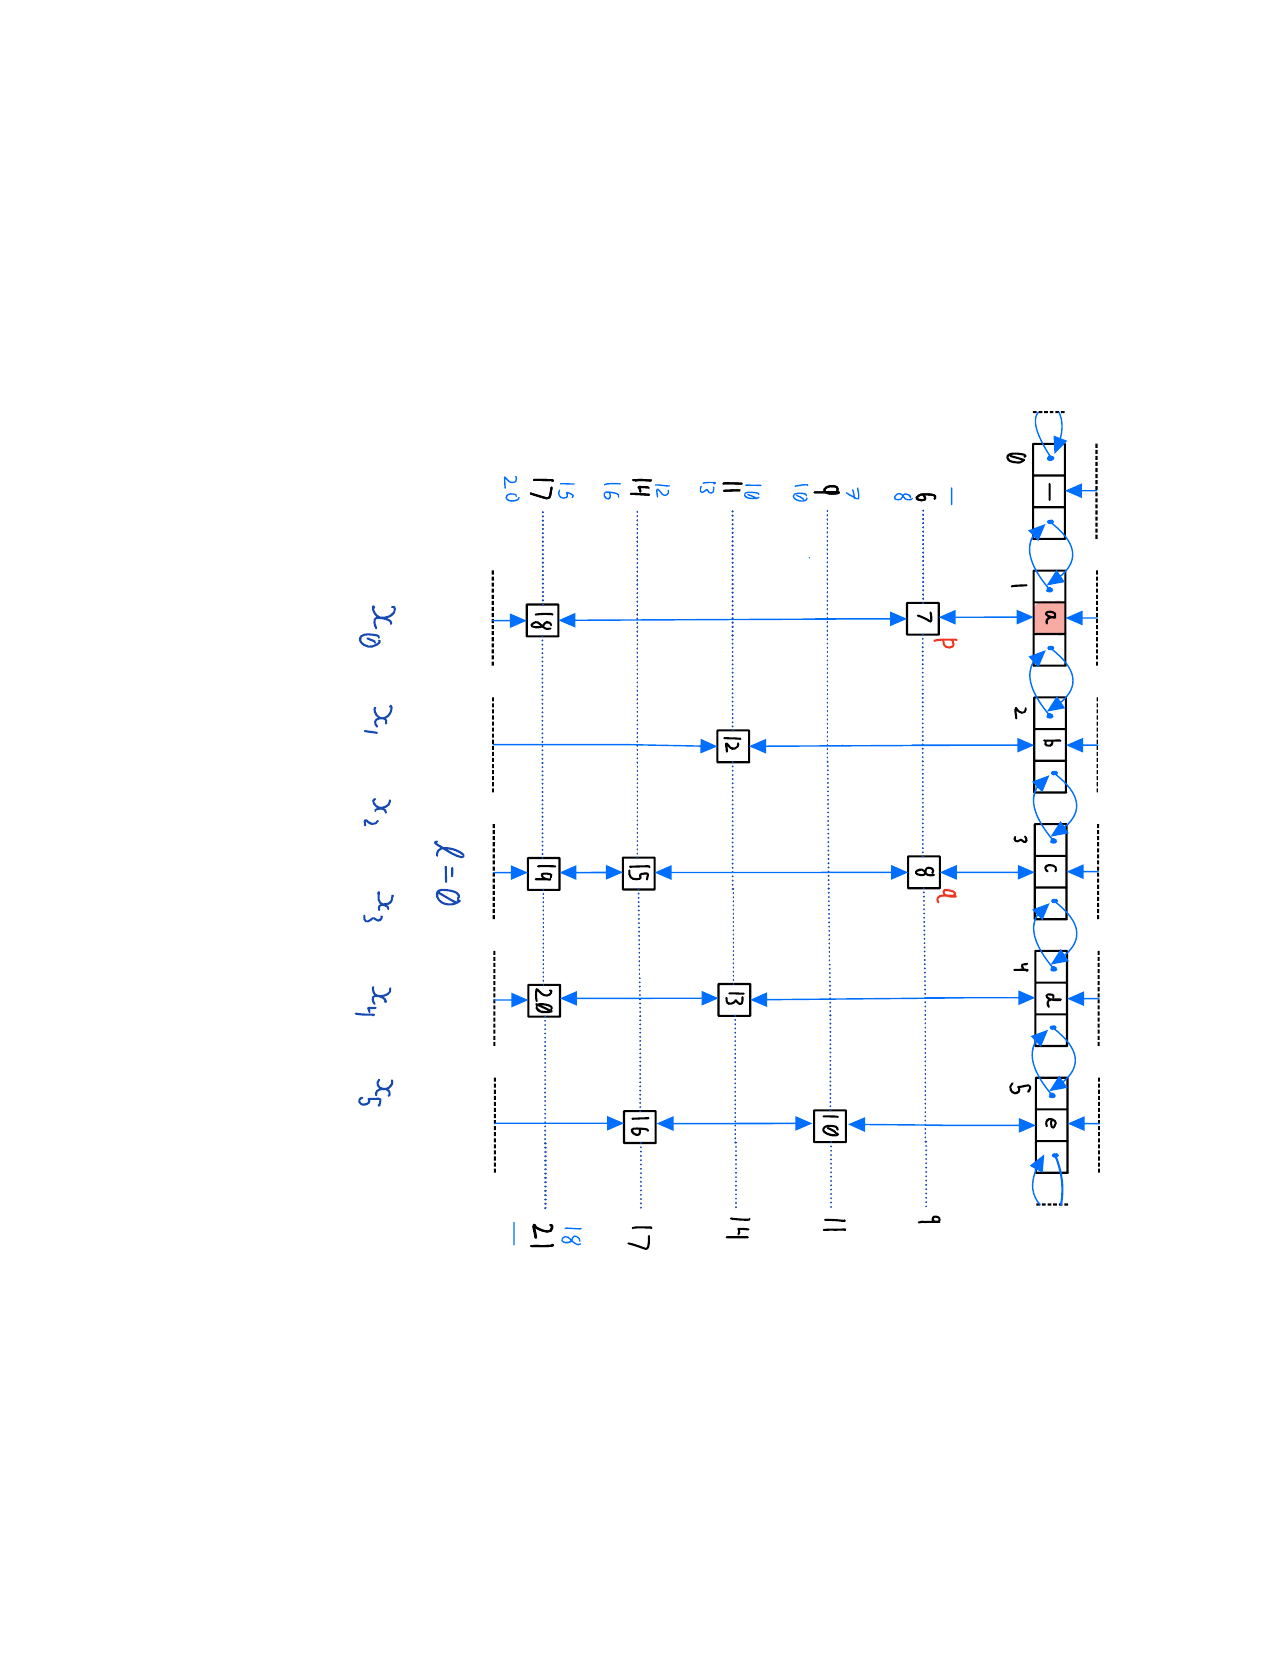
\includegraphics[angle=90,origin=c,scale=0.525]{images/Algorithm_X-05.png}} 
\begin{frame}{}
    \vspace{-130pt}
    Select $i=a$, cover($a$)
\end{frame} 
}

{ 
\usebackgroundtemplate{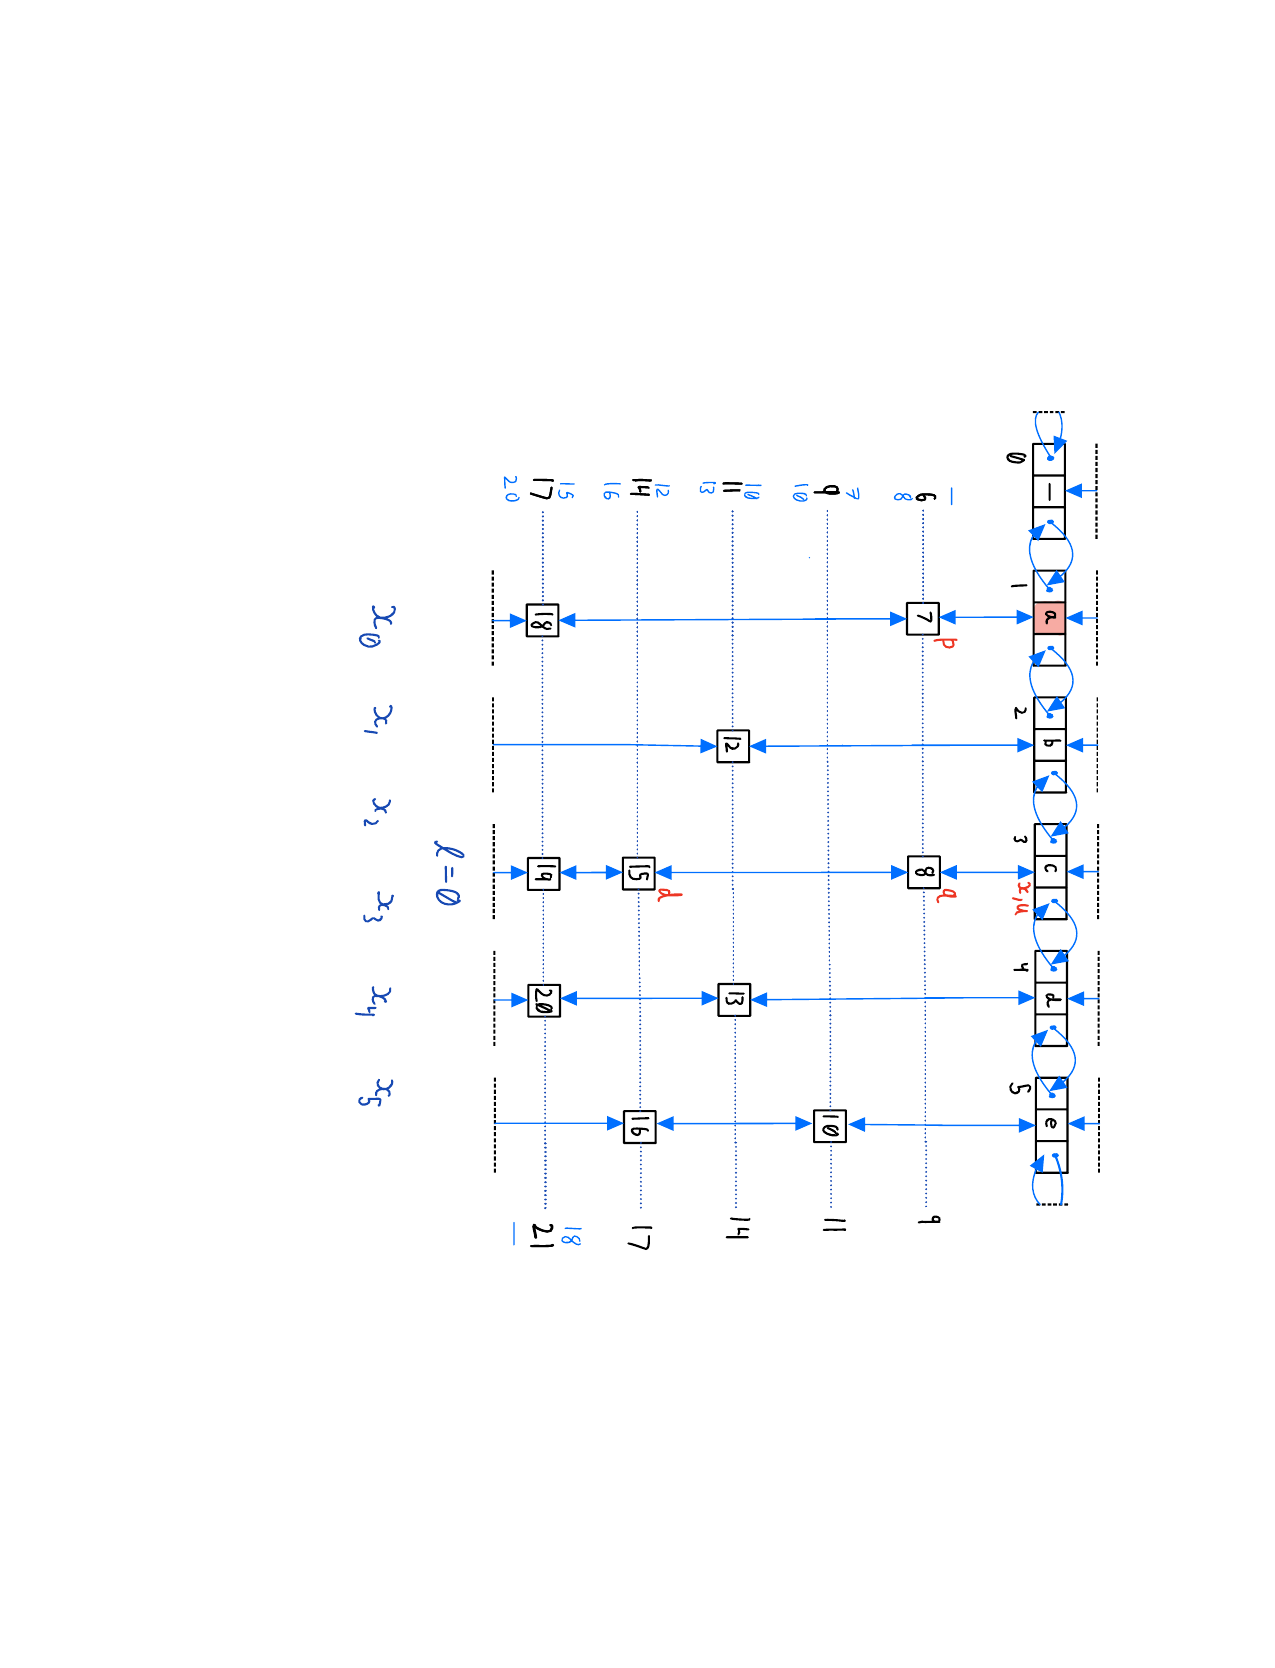
\includegraphics[angle=90,origin=c,scale=0.525]{images/Algorithm_X-06.png}} 
\begin{frame}{}
    \vspace{-130pt}
    hide($7$)
\end{frame} 
}

{ 
\usebackgroundtemplate{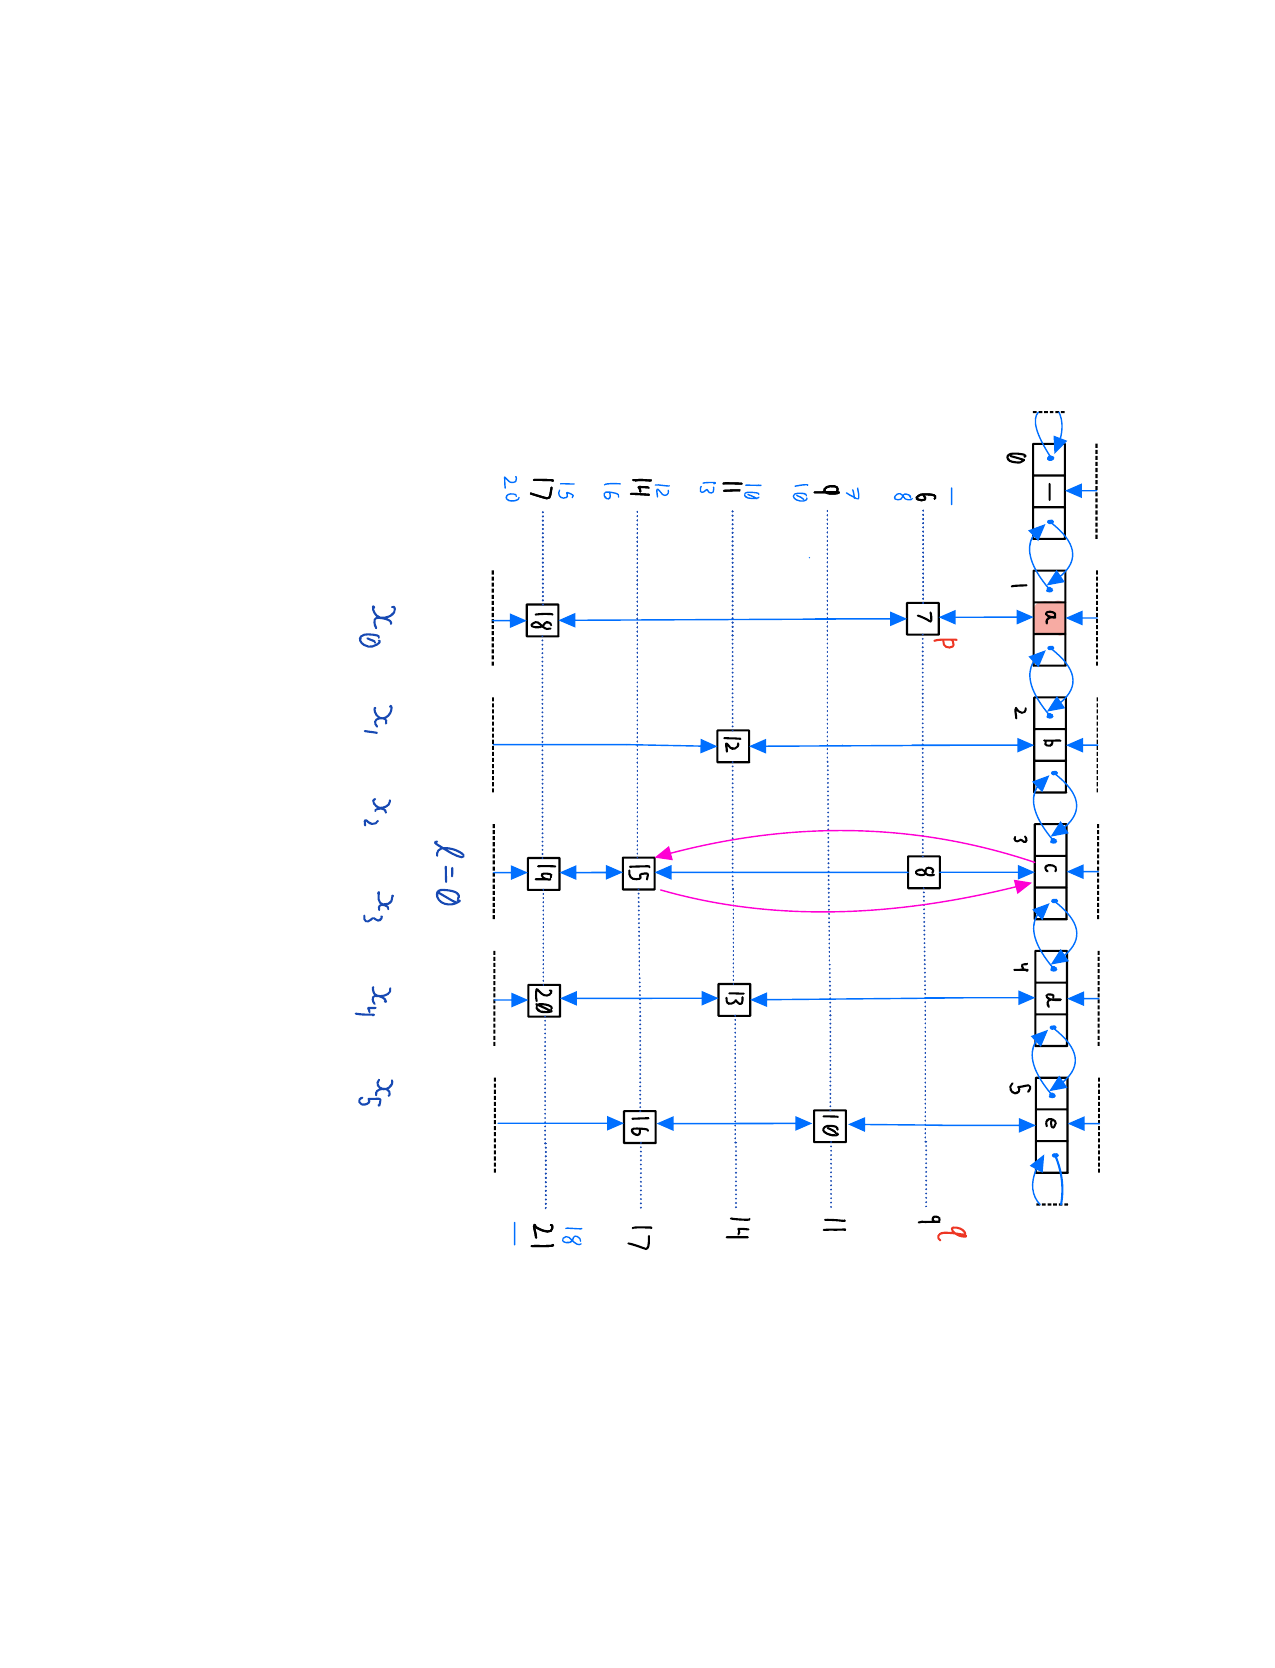
\includegraphics[angle=90,origin=c,scale=0.525]{images/Algorithm_X-07.png}} 
\begin{frame}{}
    \vspace{-130pt}
    hide($7$)
\end{frame} 
}

{ 
\usebackgroundtemplate{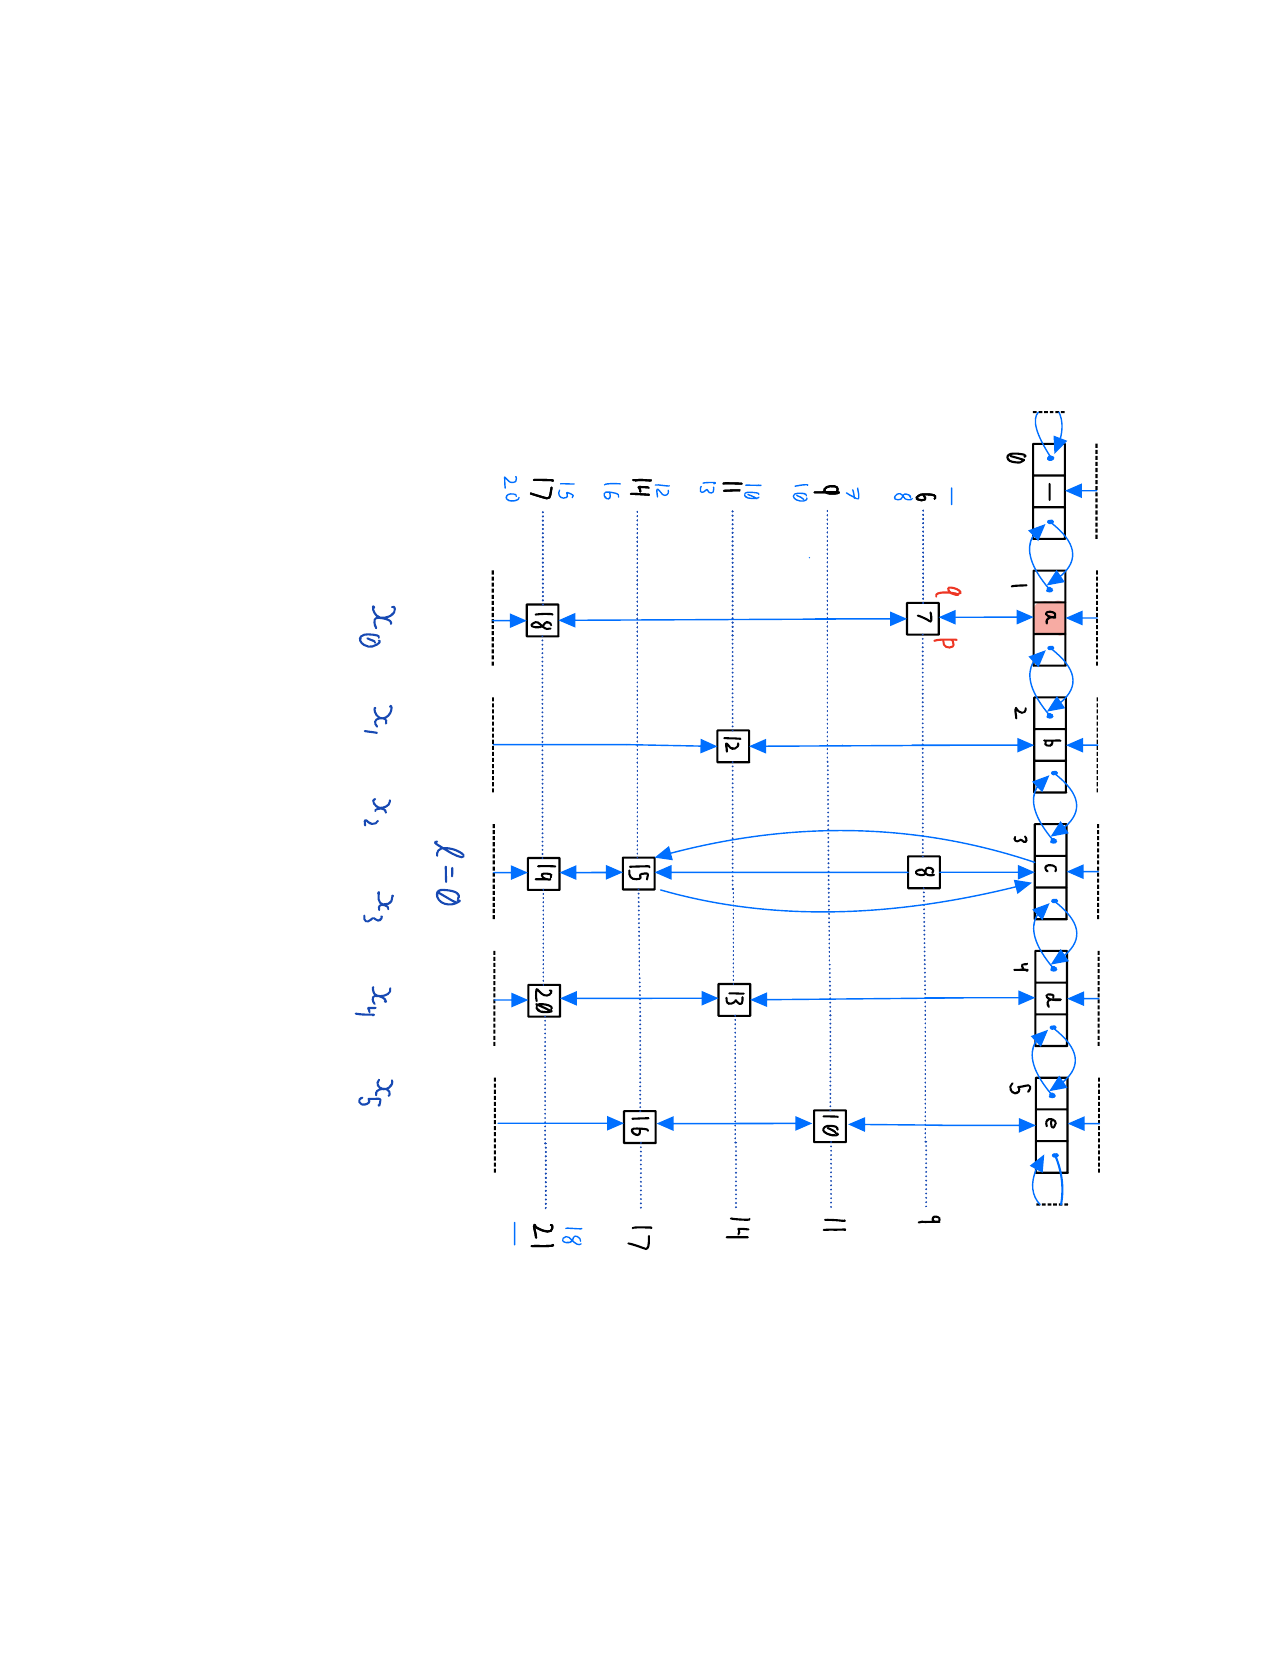
\includegraphics[angle=90,origin=c,scale=0.525]{images/Algorithm_X-08.png}} 
\begin{frame}{}
    \vspace{-130pt}
    hide($7$)
\end{frame} 
}

{ 
\usebackgroundtemplate{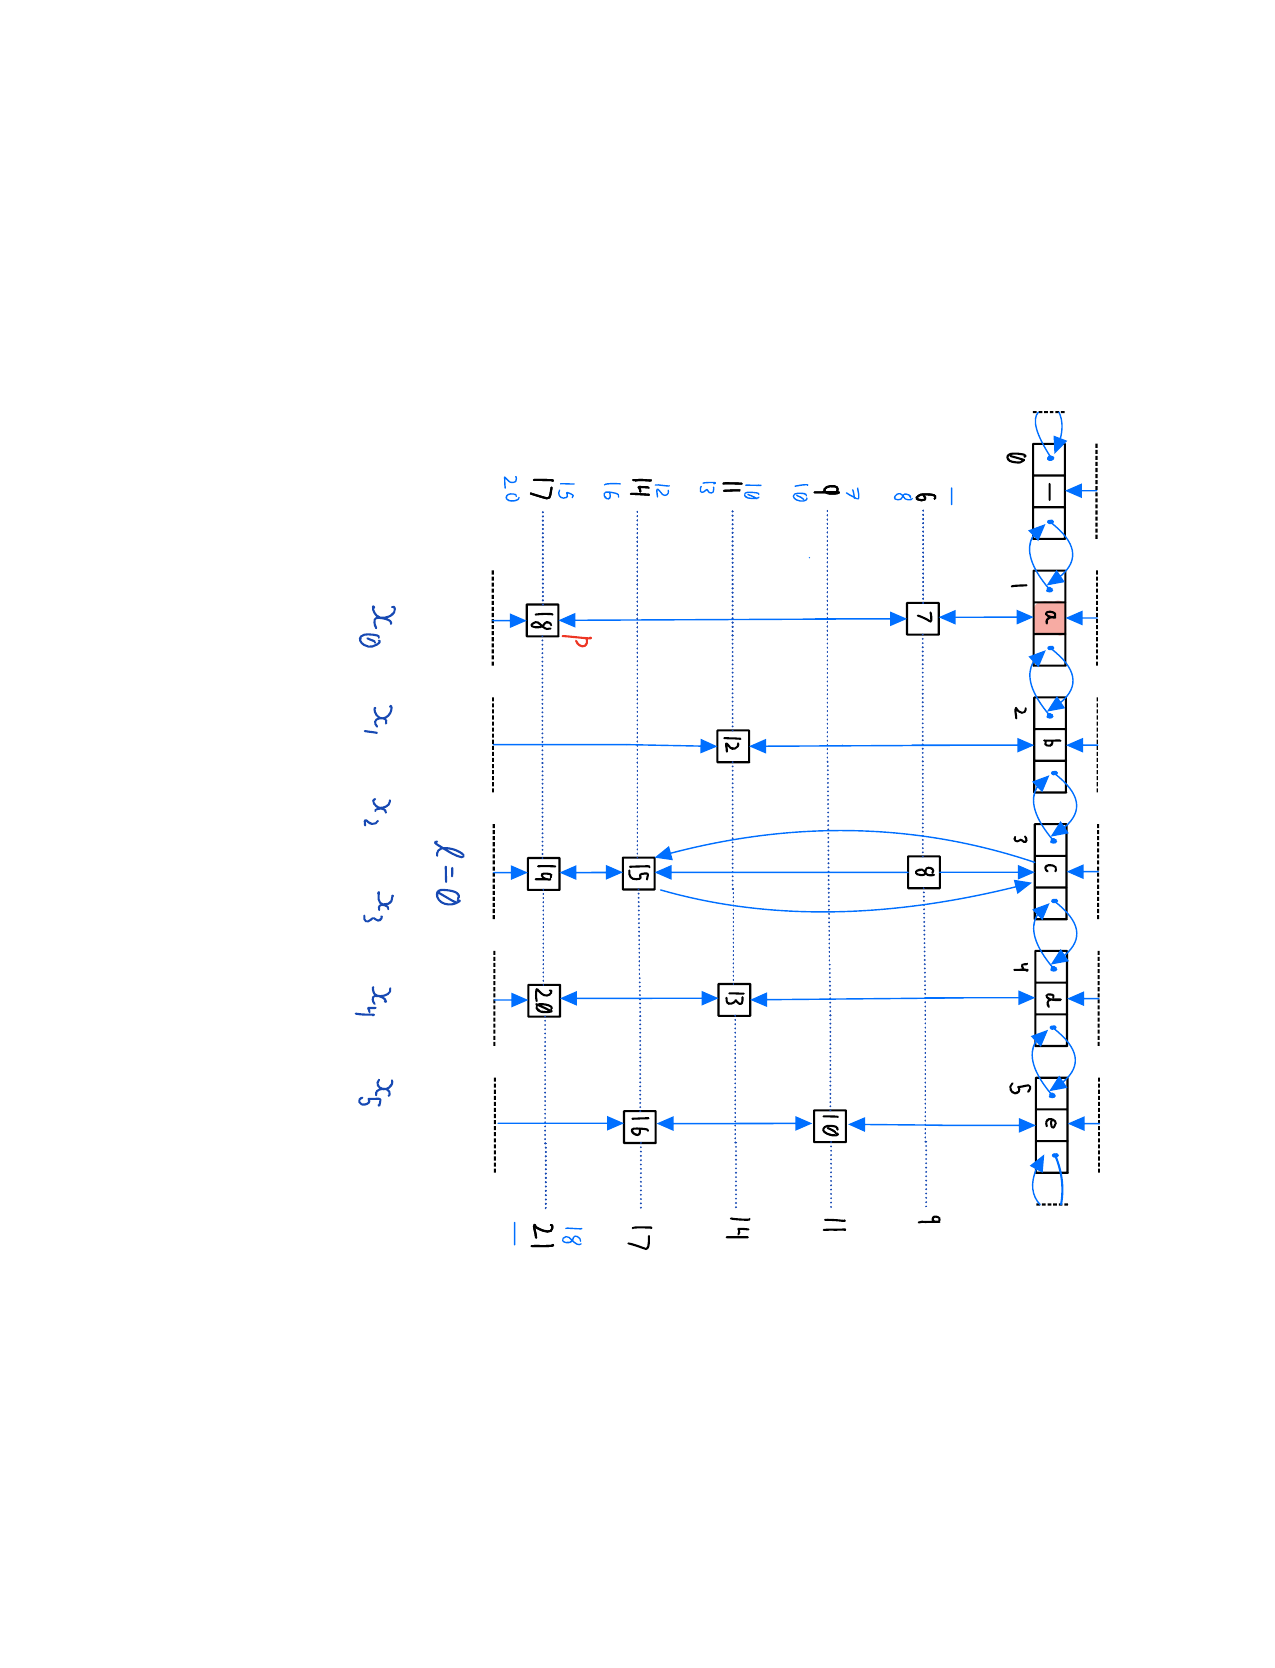
\includegraphics[angle=90,origin=c,scale=0.525]{images/Algorithm_X-09.png}} 
\begin{frame}{}
    \vspace{-130pt}
    hide($18$)
\end{frame} 
}

{ 
\usebackgroundtemplate{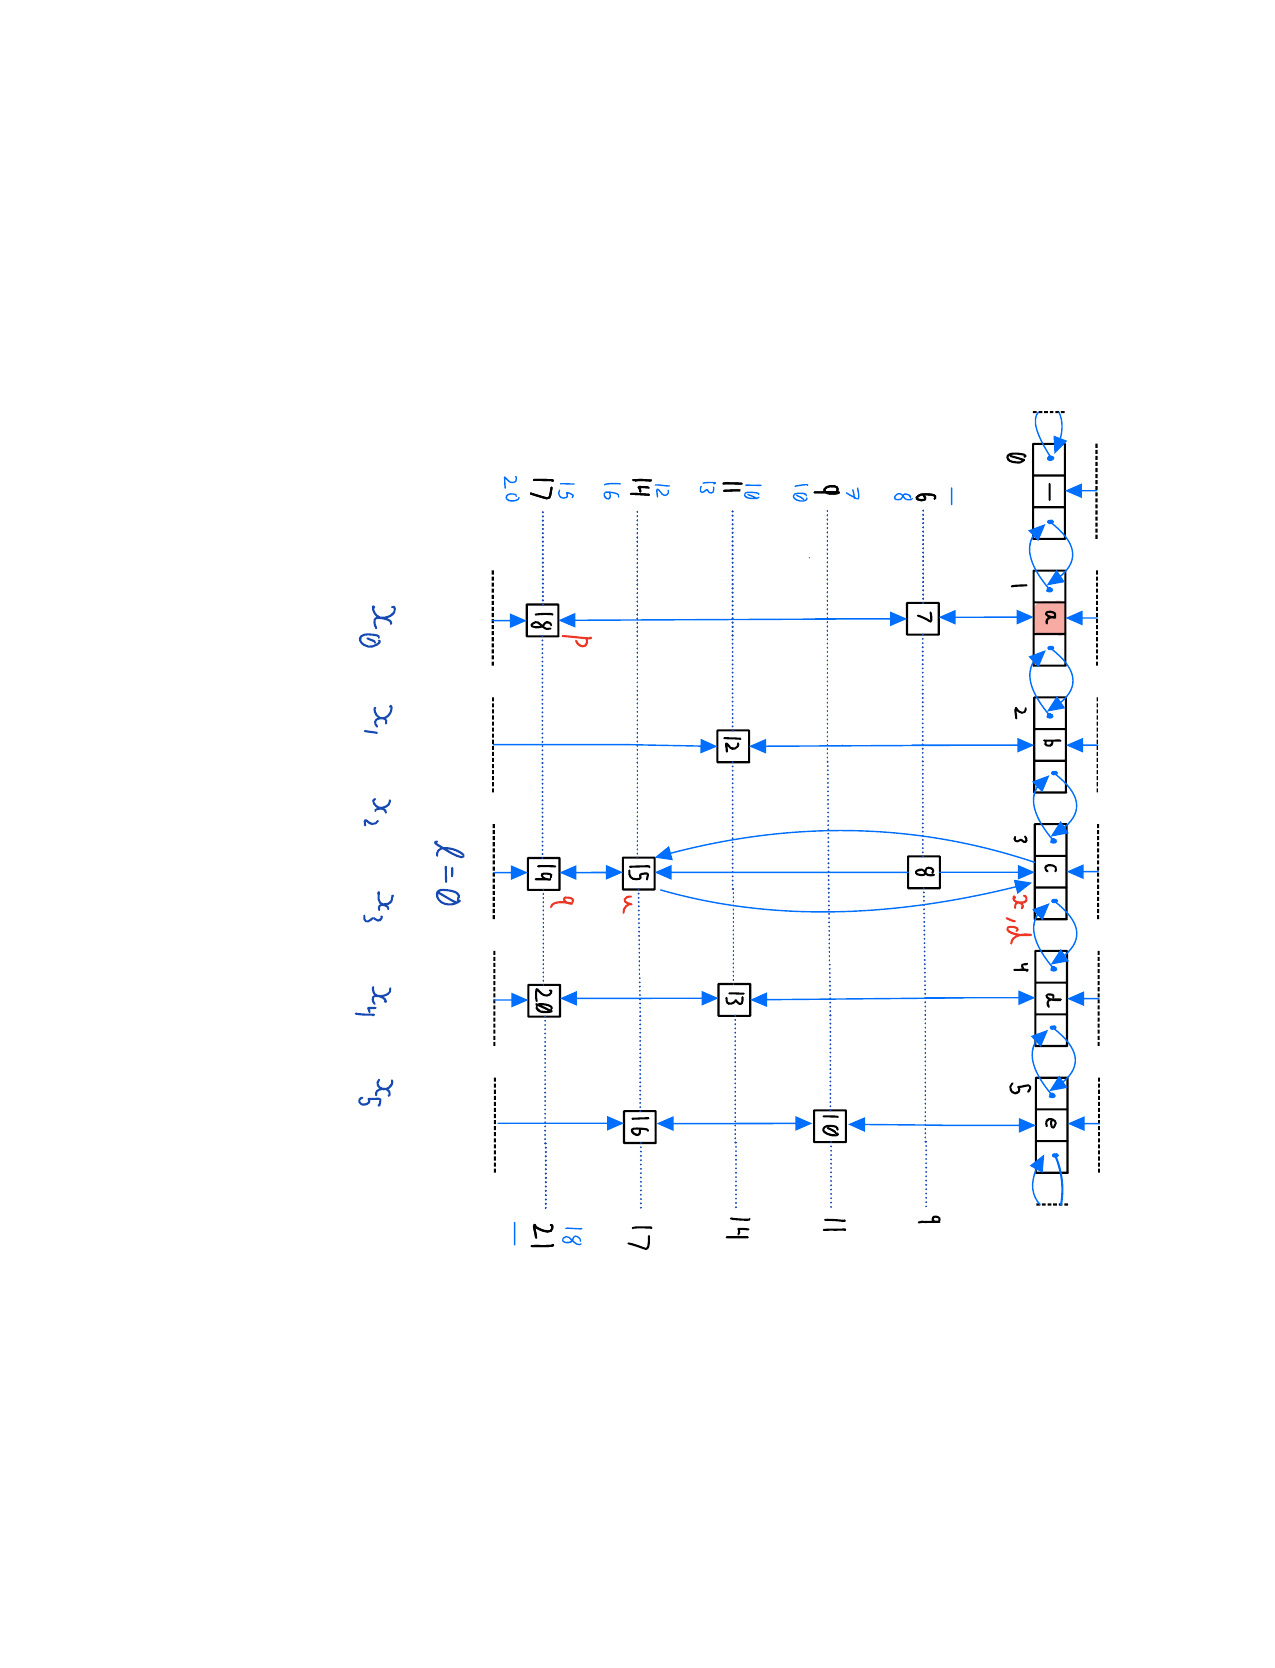
\includegraphics[angle=90,origin=c,scale=0.525]{images/Algorithm_X-10.png}} 
\begin{frame}{}
    \vspace{-130pt}
    hide($18$)
\end{frame} 
}

{ 
\usebackgroundtemplate{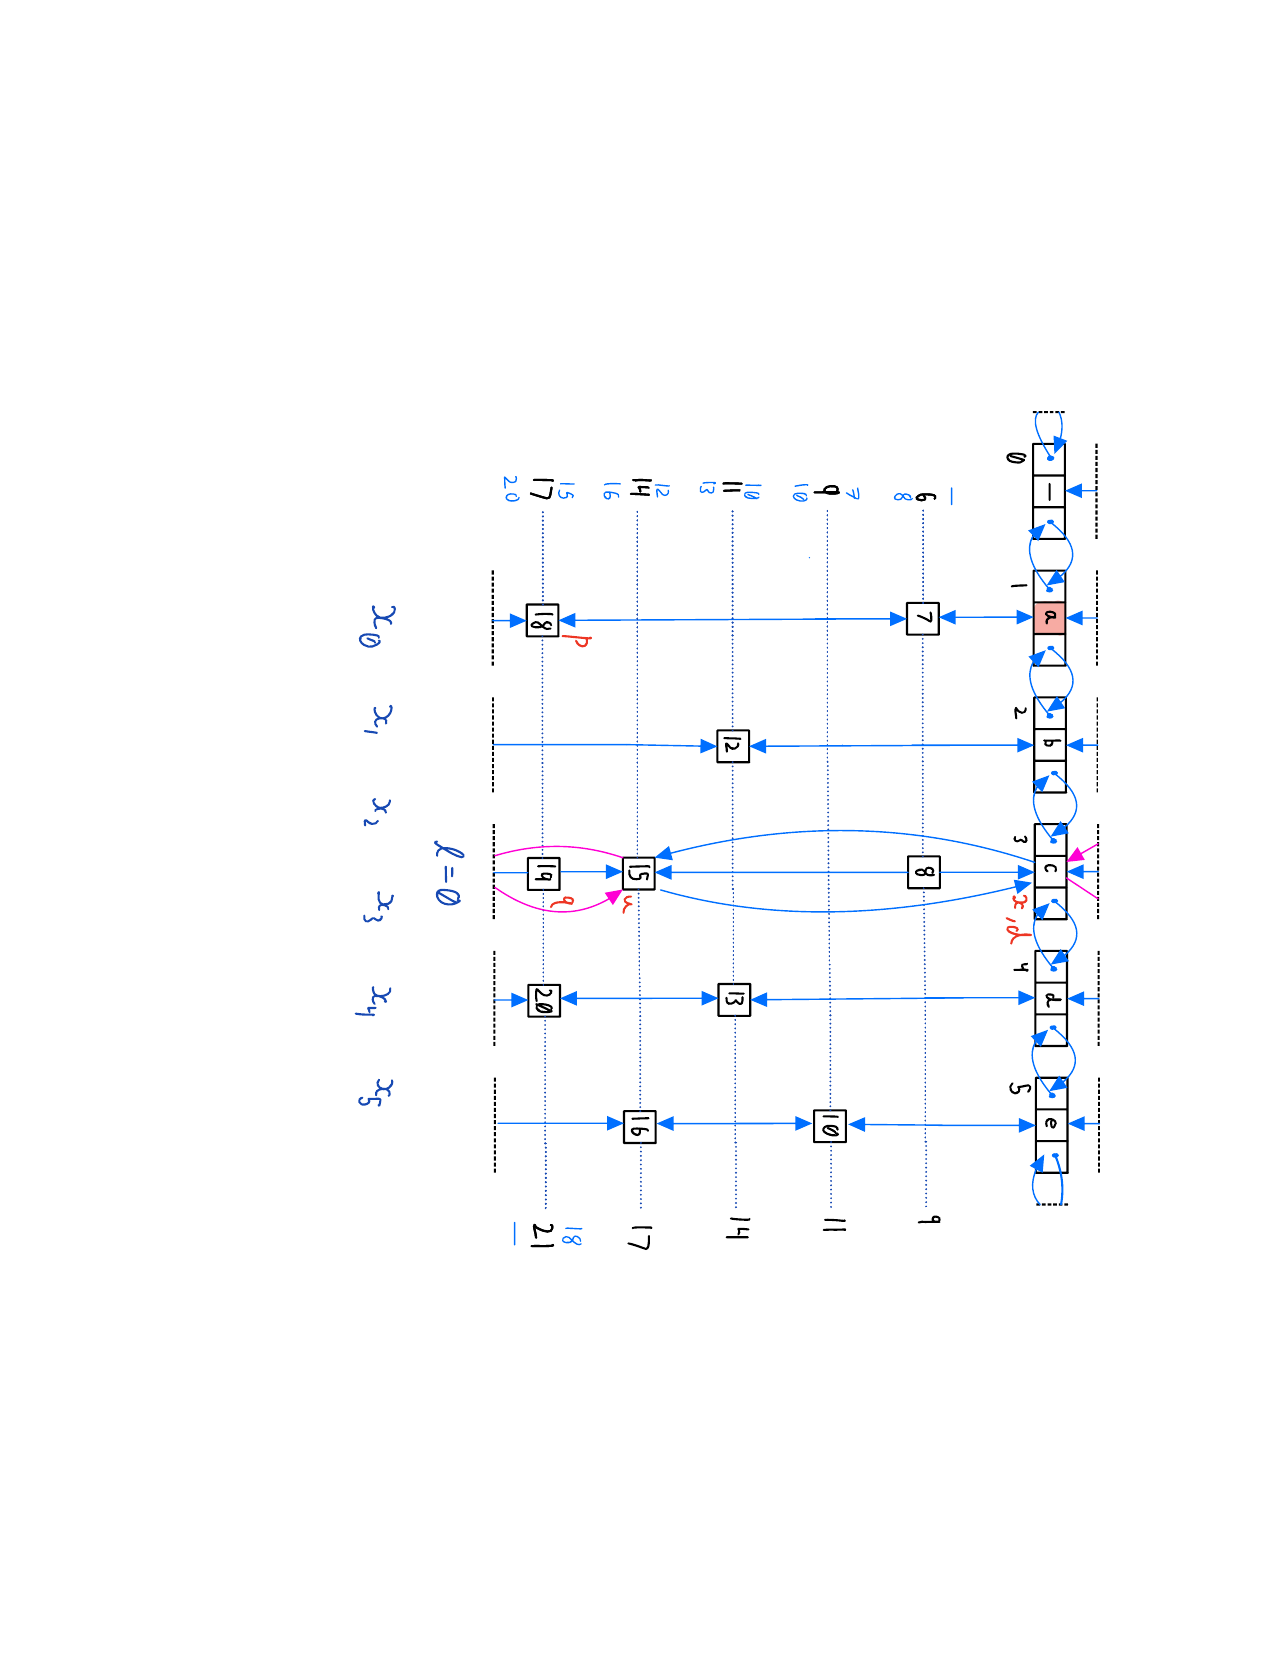
\includegraphics[angle=90,origin=c,scale=0.525]{images/Algorithm_X-11.png}} 
\begin{frame}{}
    \vspace{-130pt}
    hide($18$)
\end{frame} 
}

{ 
\usebackgroundtemplate{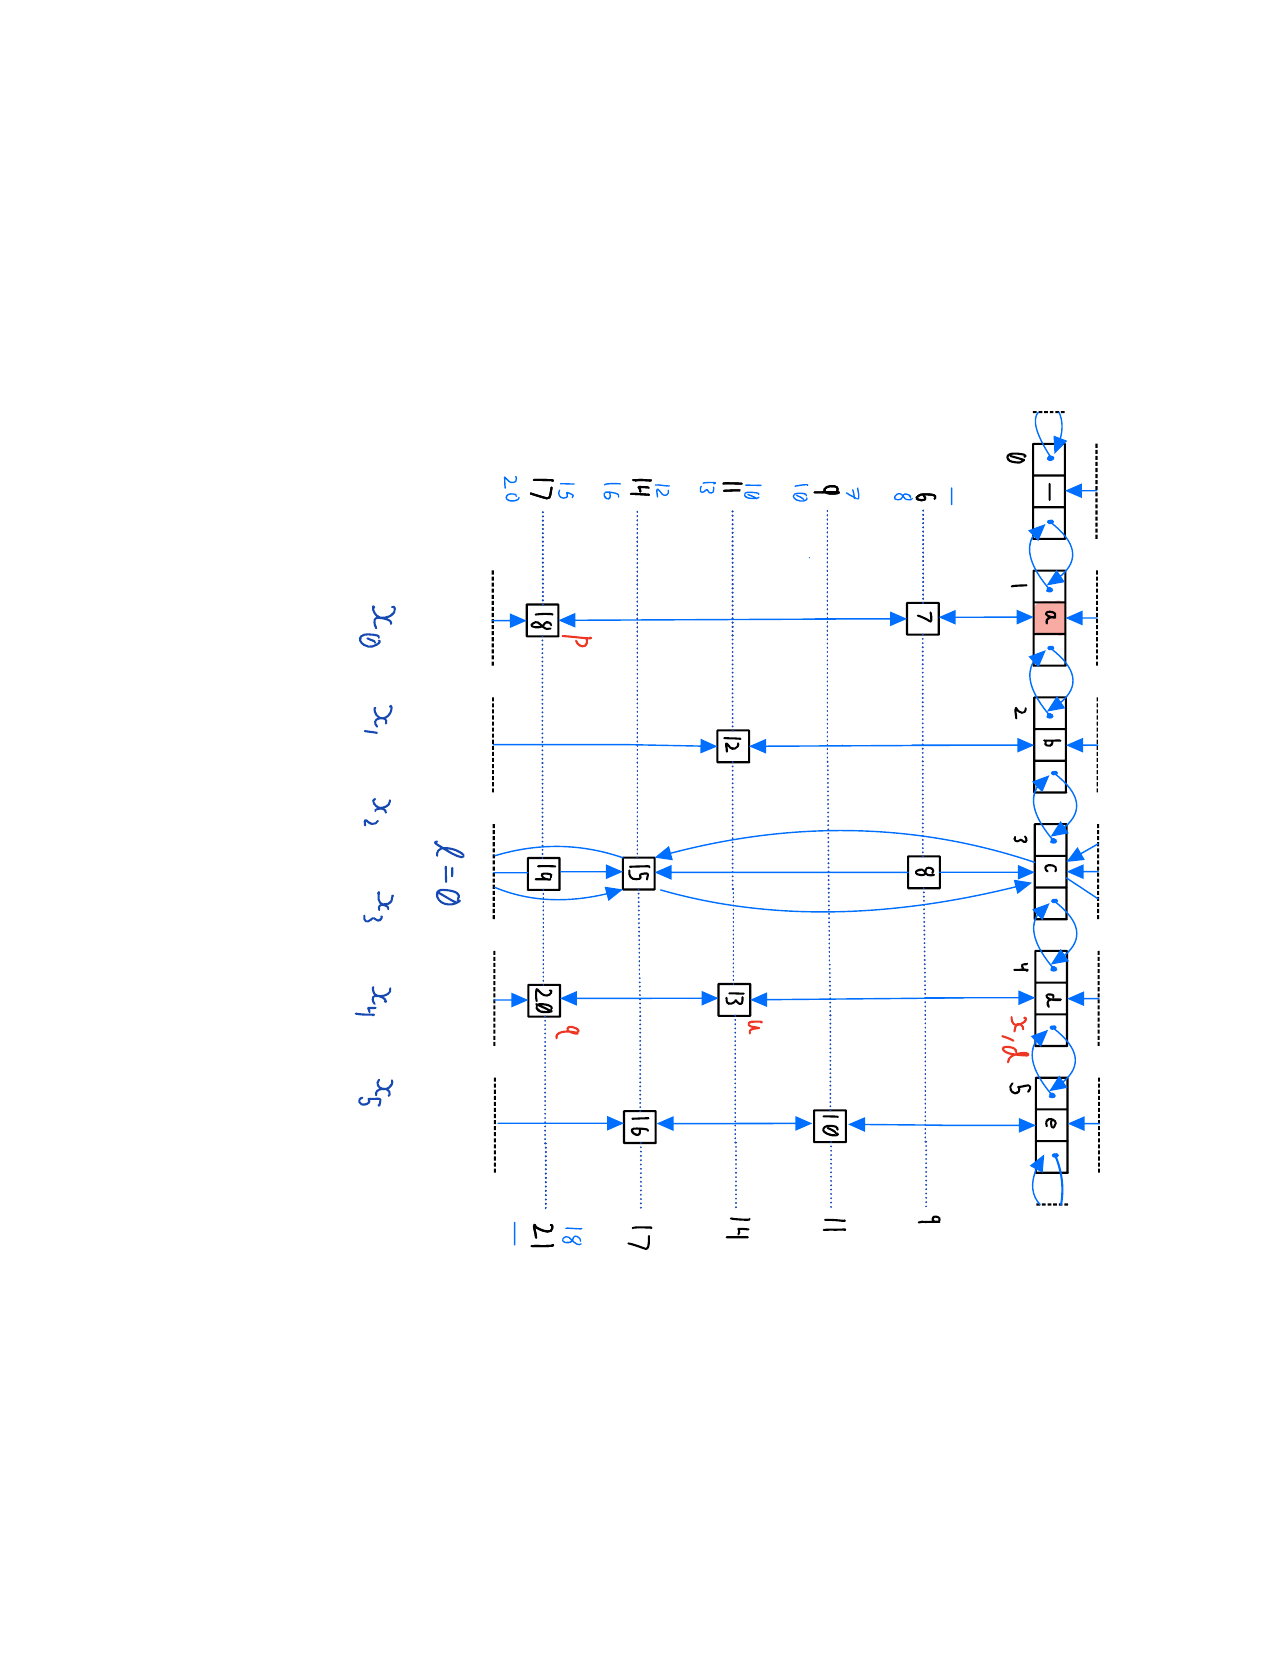
\includegraphics[angle=90,origin=c,scale=0.525]{images/Algorithm_X-12.png}} 
\begin{frame}{}
    \vspace{-130pt}
    hide($18$)
\end{frame} 
}

{ 
\usebackgroundtemplate{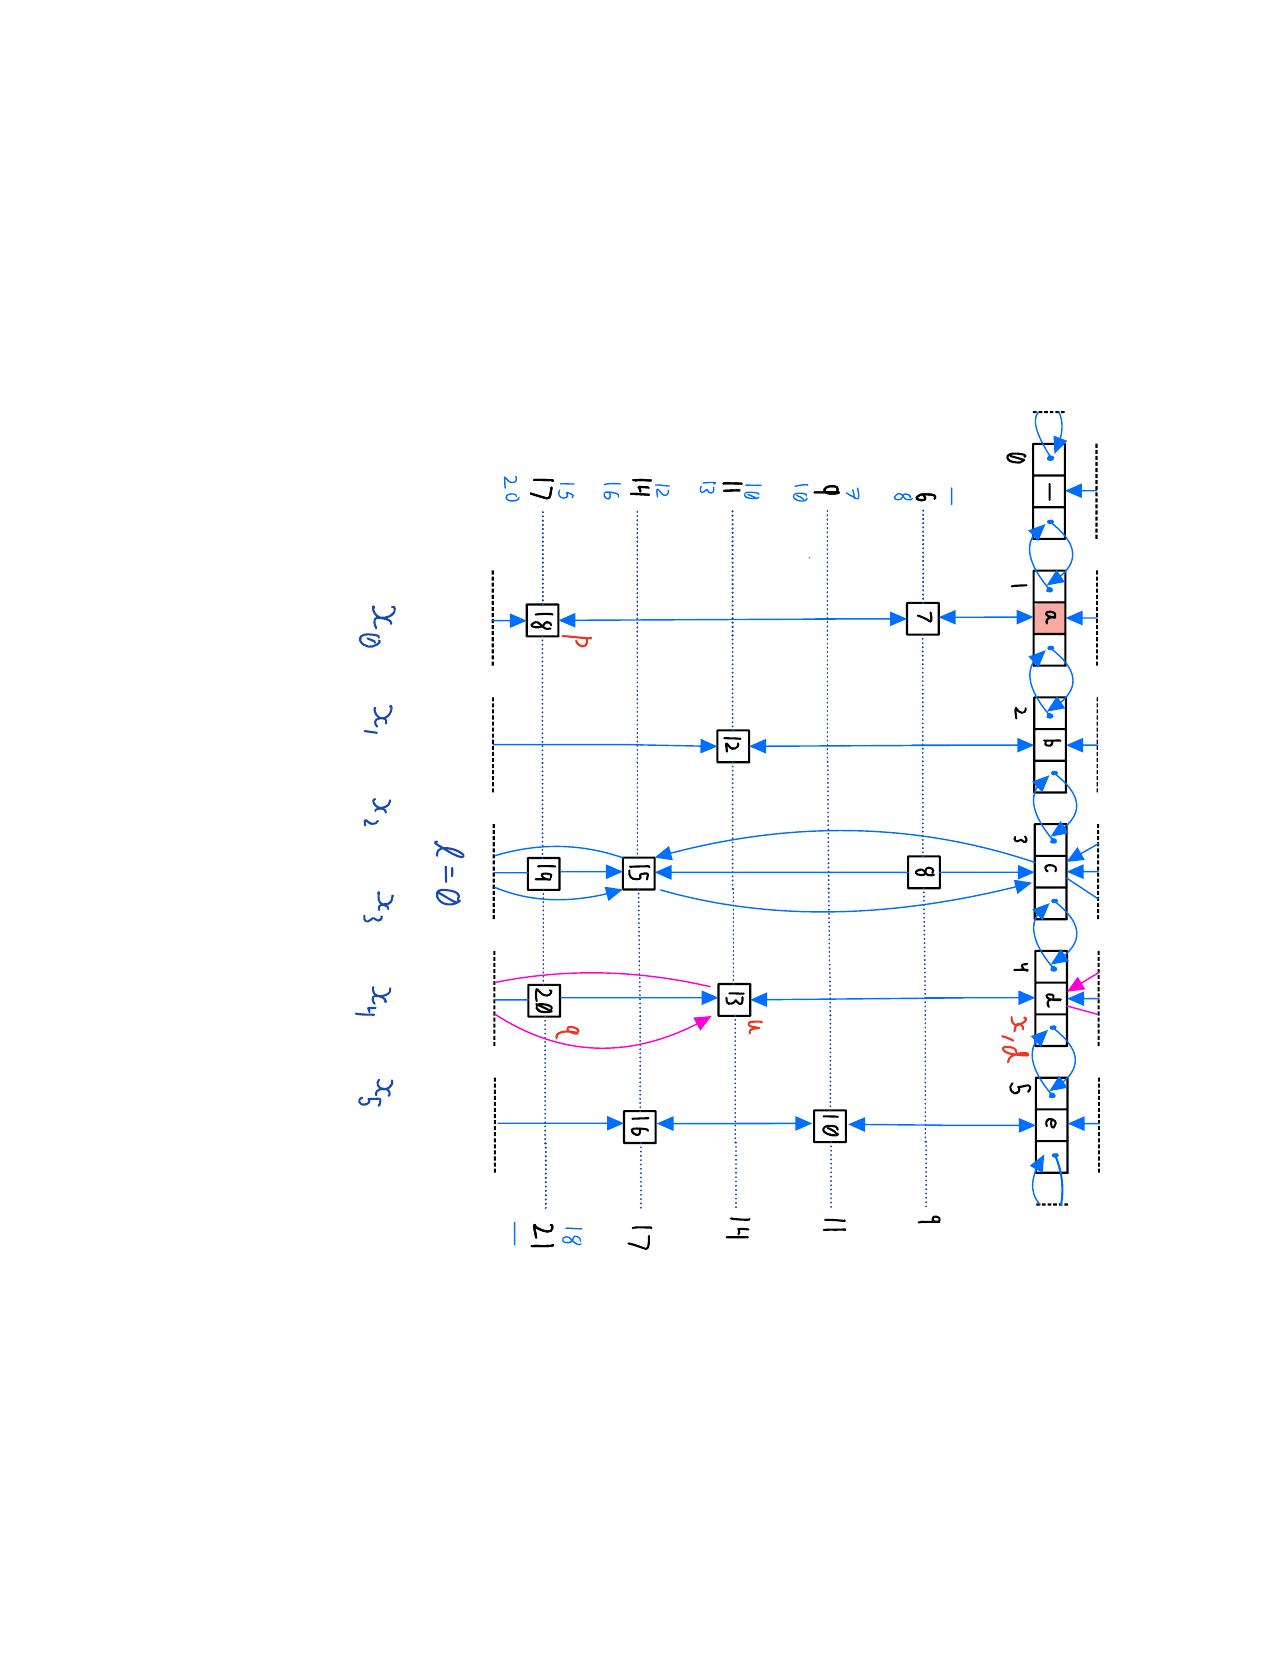
\includegraphics[angle=90,origin=c,scale=0.525]{images/Algorithm_X-13.png}} 
\begin{frame}{}
    \vspace{-130pt}
    hide($18$)
\end{frame} 
}

{ 
\usebackgroundtemplate{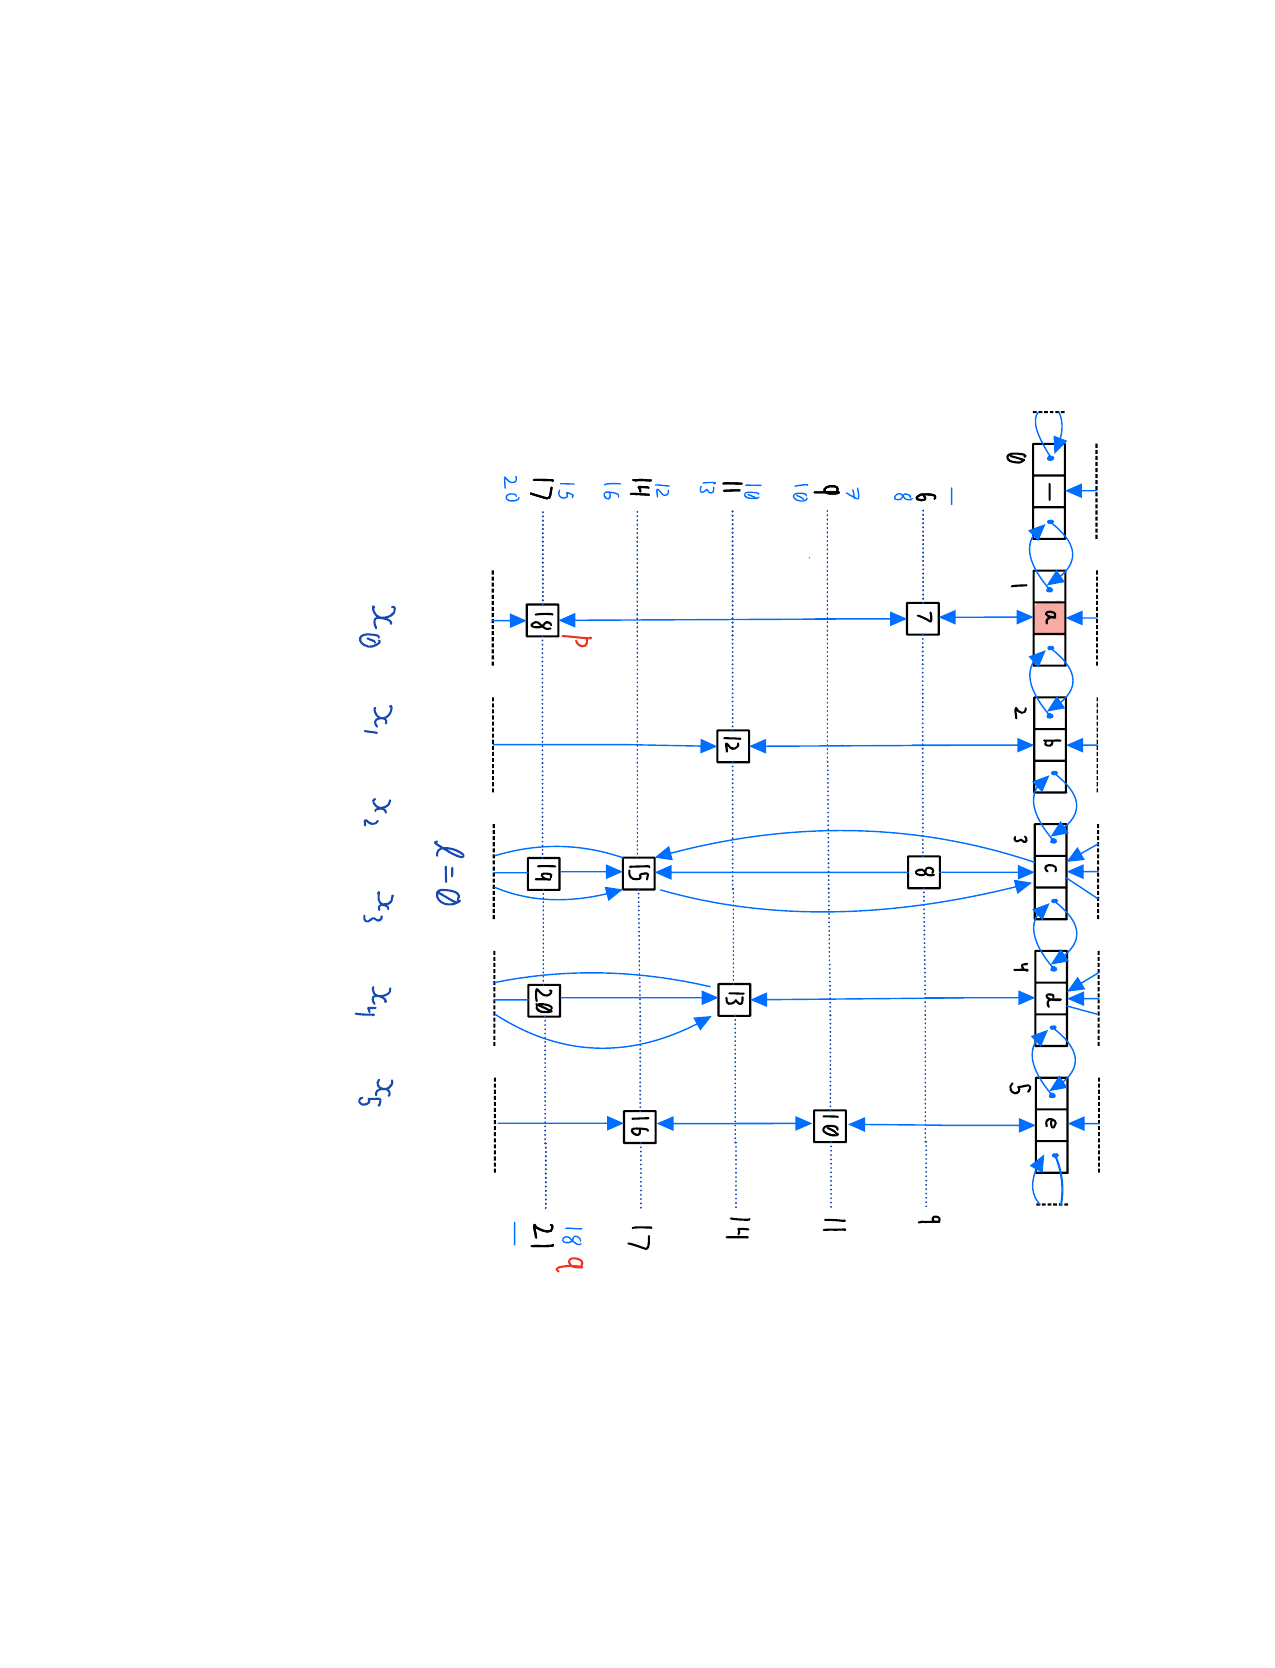
\includegraphics[angle=90,origin=c,scale=0.525]{images/Algorithm_X-14.png}} 
\begin{frame}{}
    \vspace{-130pt}
    hide($18$)
\end{frame} 
}

{ 
\usebackgroundtemplate{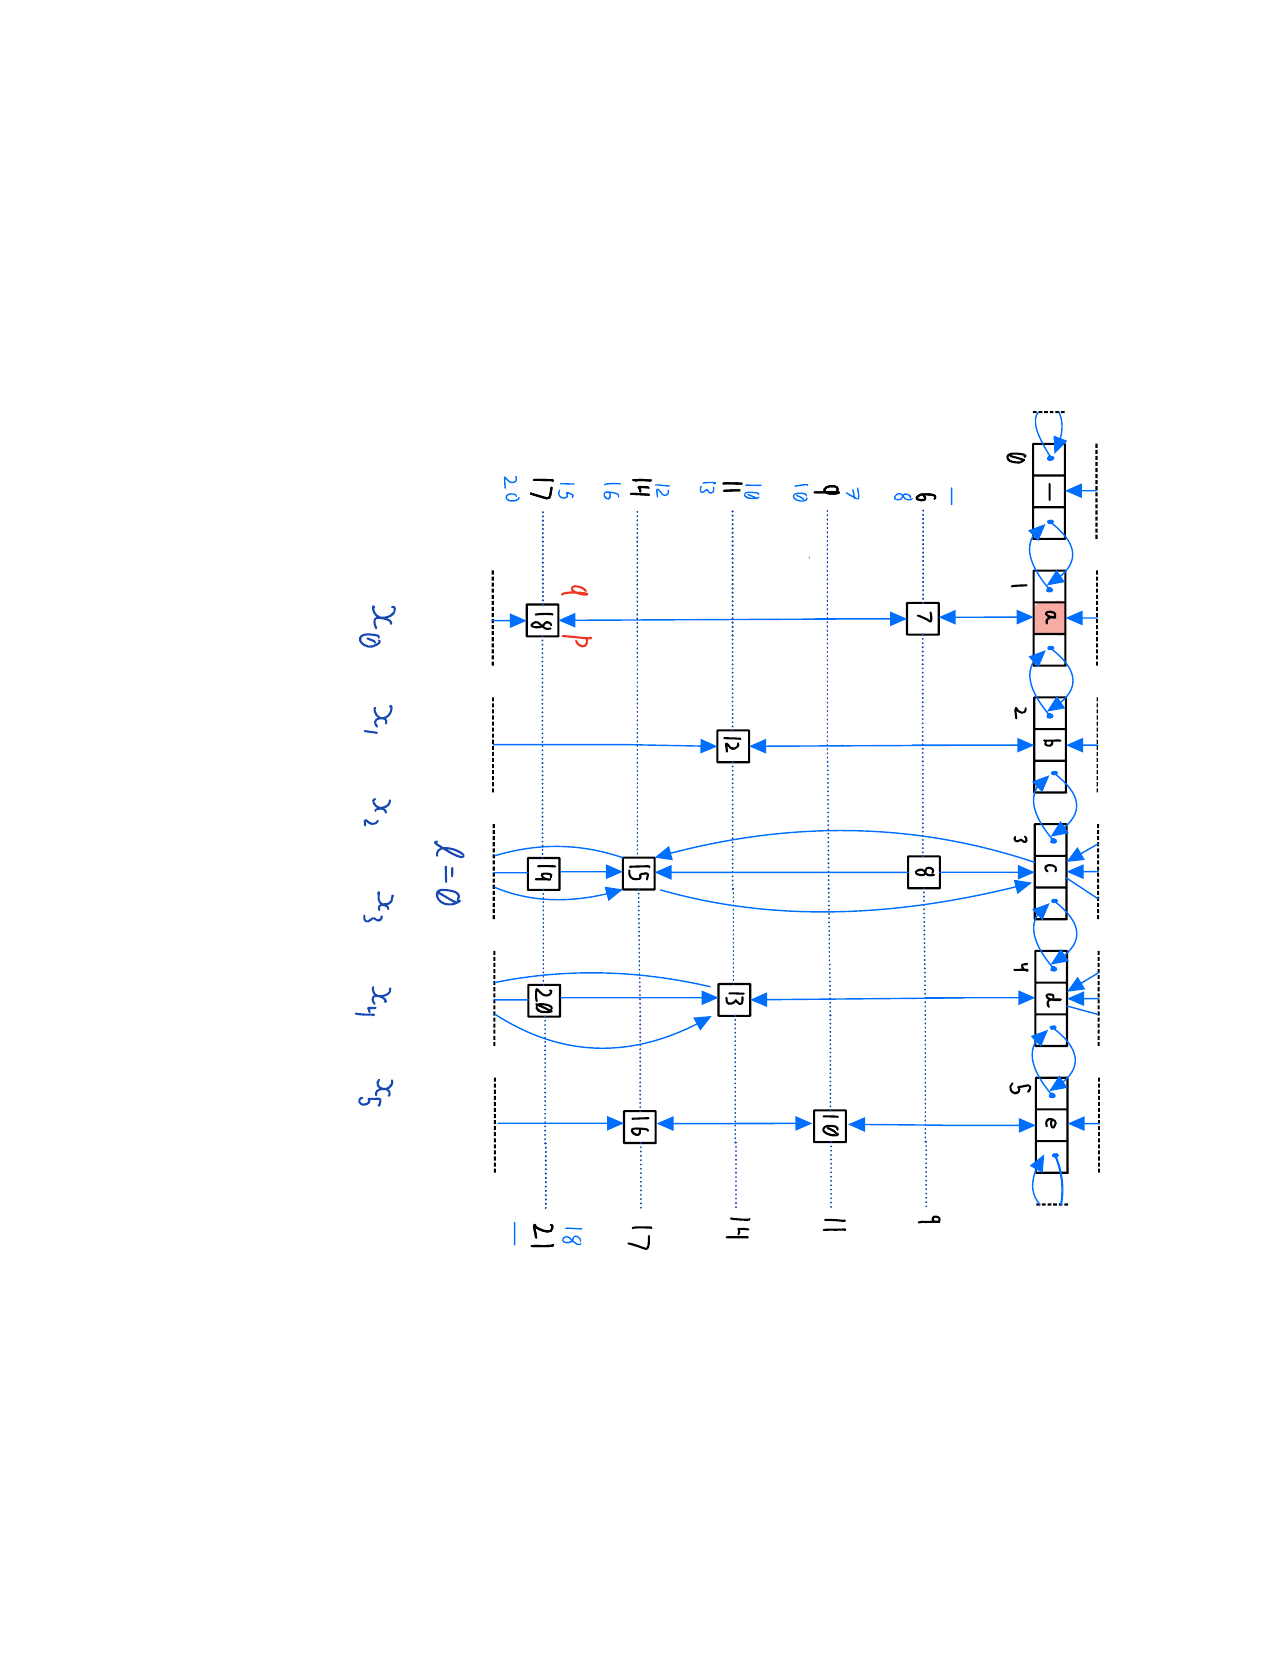
\includegraphics[angle=90,origin=c,scale=0.525]{images/Algorithm_X-15.png}} 
\begin{frame}{}
    \vspace{-130pt}
    hide($18$)
\end{frame} 
}

{ 
\usebackgroundtemplate{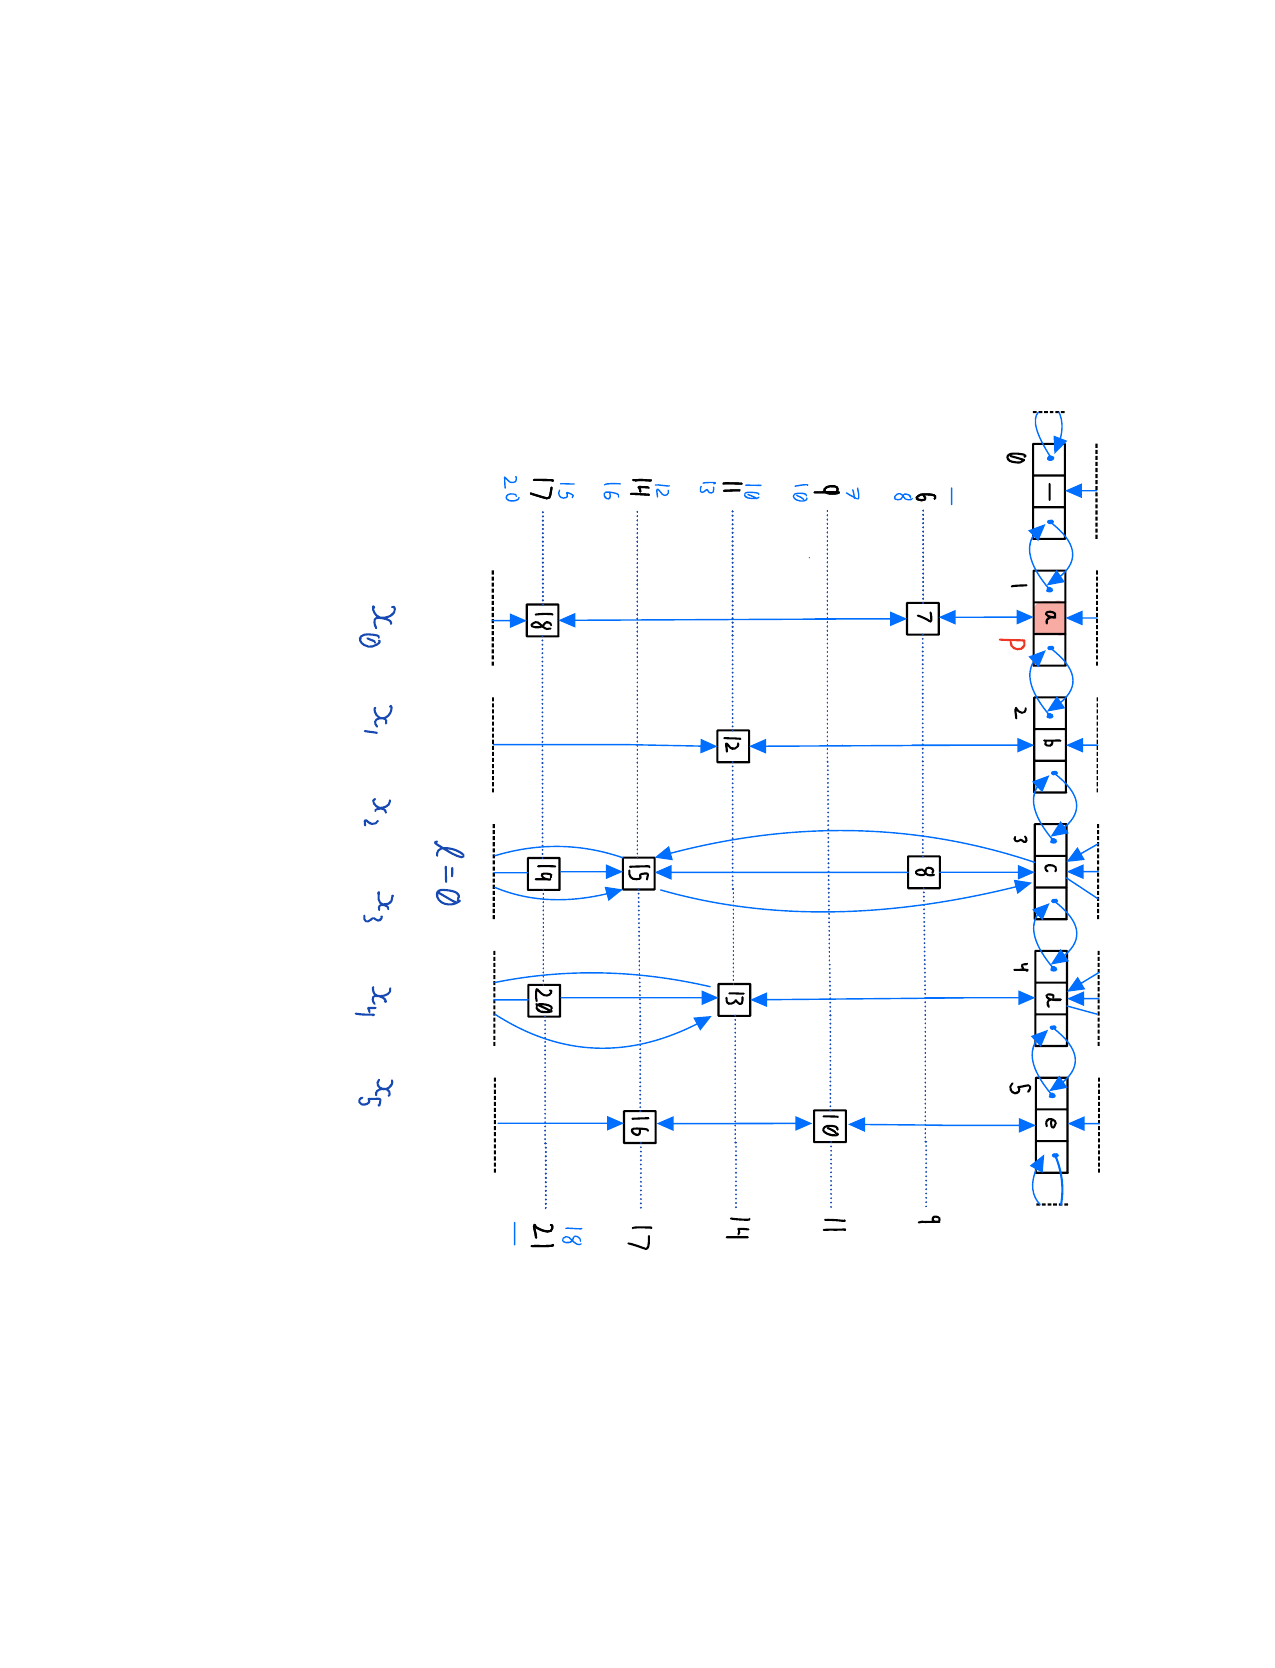
\includegraphics[angle=90,origin=c,scale=0.525]{images/Algorithm_X-16.png}} 
\begin{frame}{}
    \vspace{-130pt}
    remove $a$
\end{frame} 
}

{ 
\usebackgroundtemplate{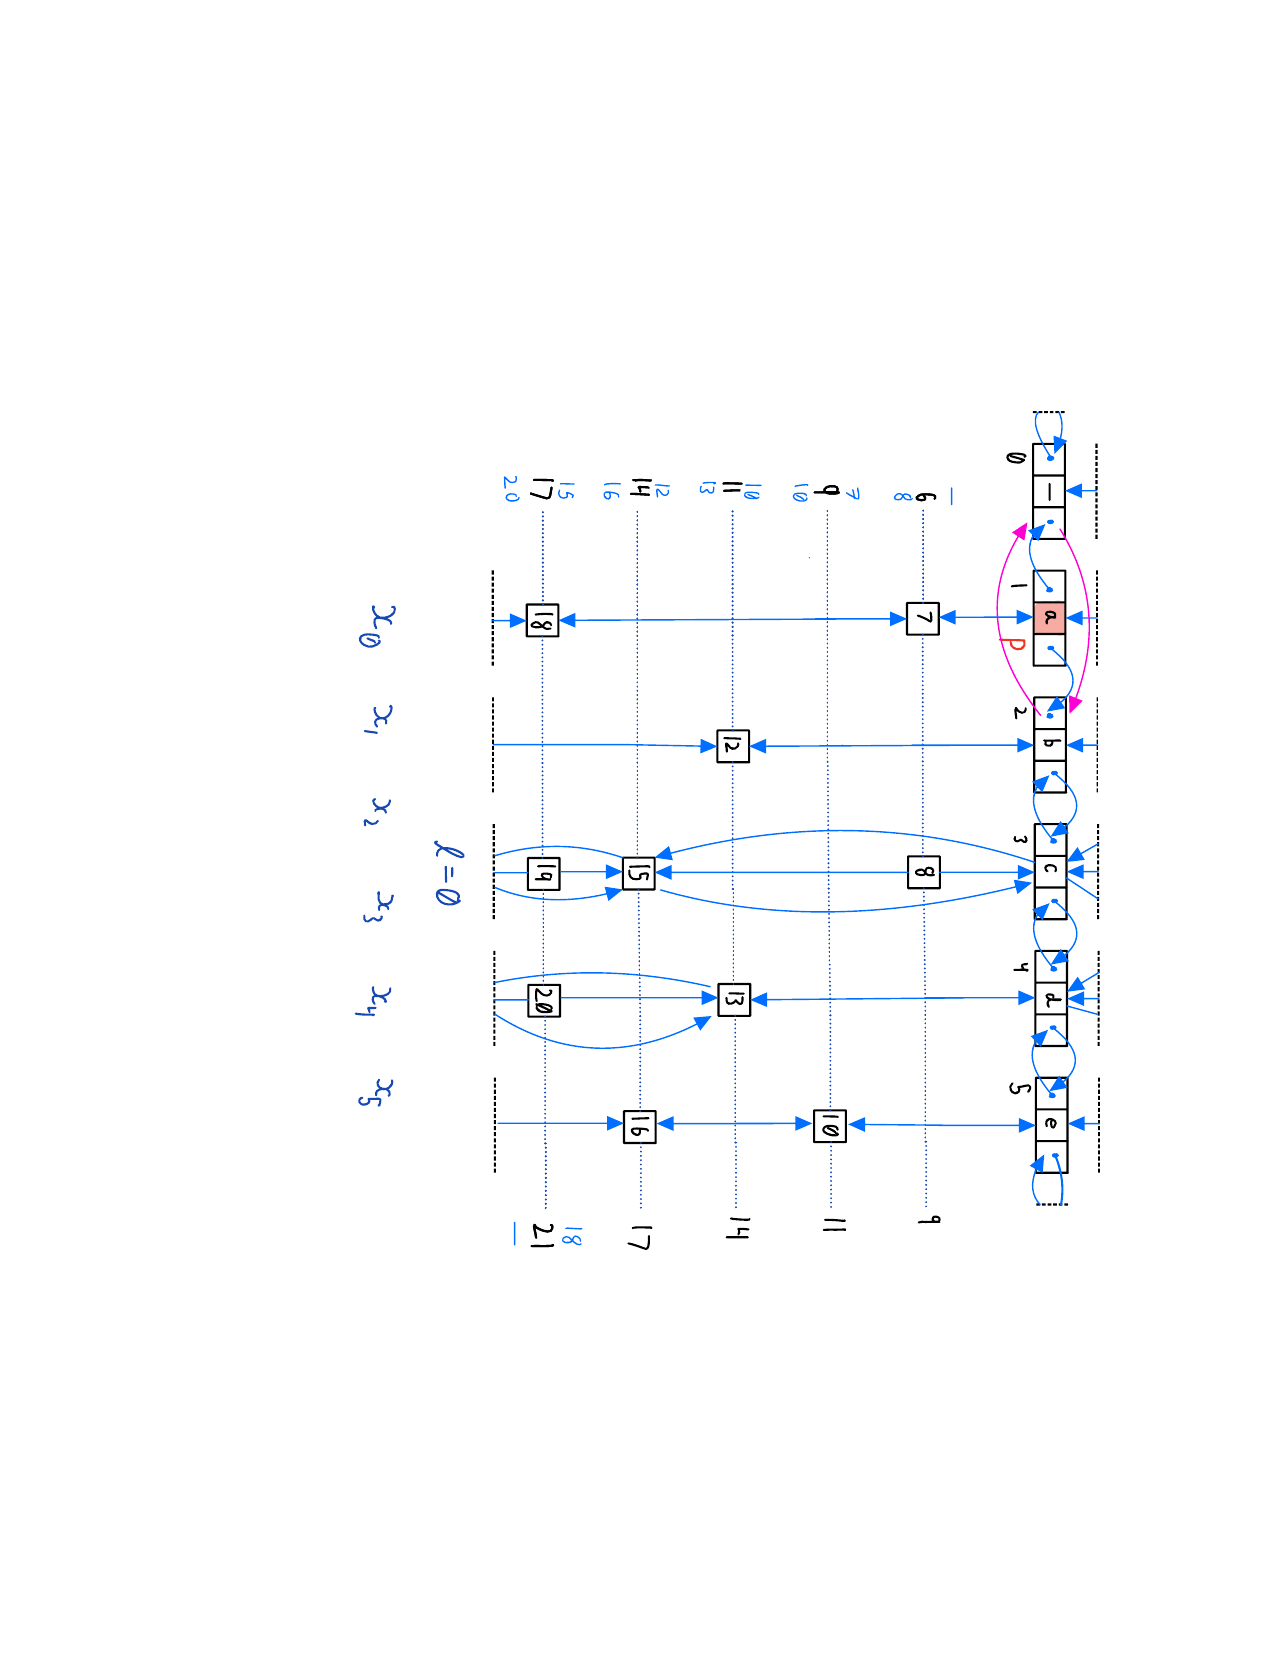
\includegraphics[angle=90,origin=c,scale=0.525]{images/Algorithm_X-17.png}} 
\begin{frame}{}
    \vspace{-130pt}
    remove $a$
\end{frame} 
}

{ 
\usebackgroundtemplate{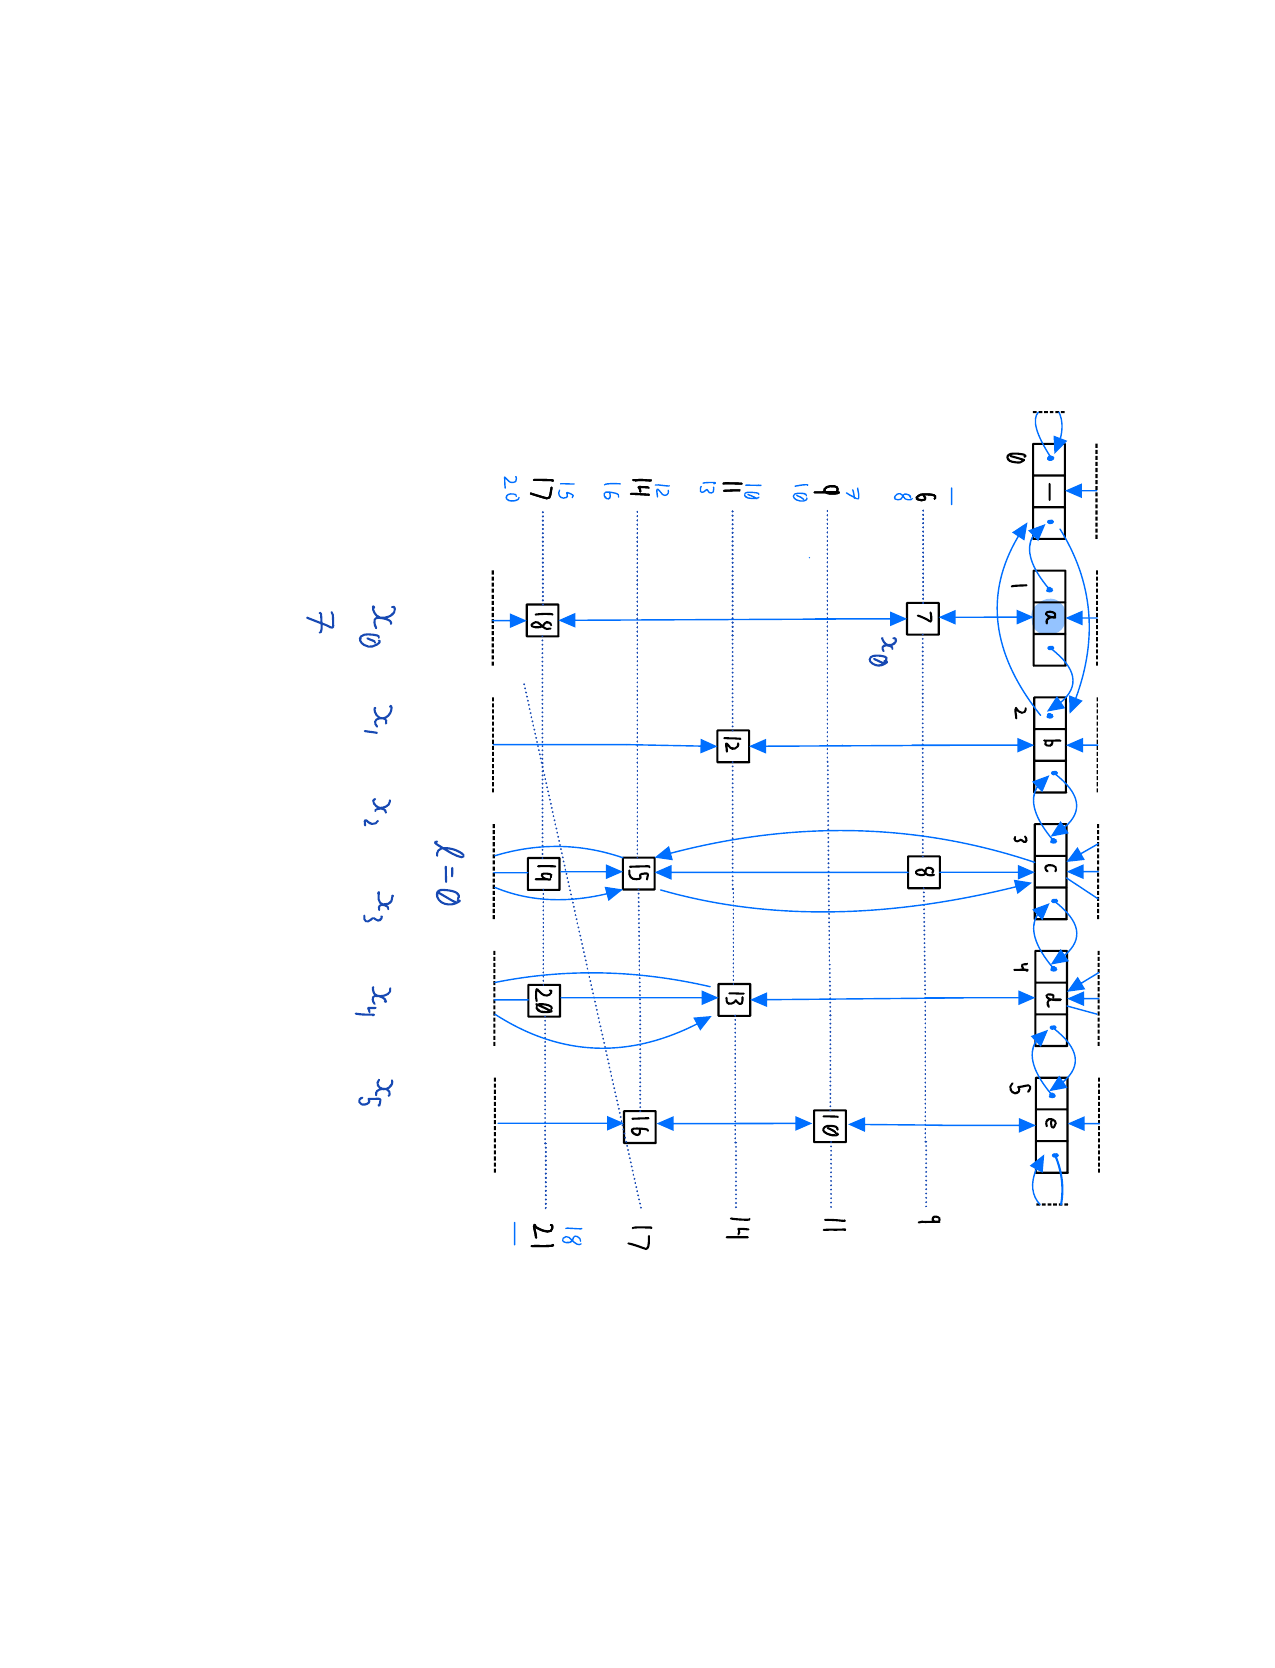
\includegraphics[angle=90,origin=c,scale=0.525]{images/Algorithm_X-18.png}} 
\begin{frame}{}
    \vspace{-130pt}
    $\ell=0$, $x_0=7$
\end{frame} 
}

{ 
\usebackgroundtemplate{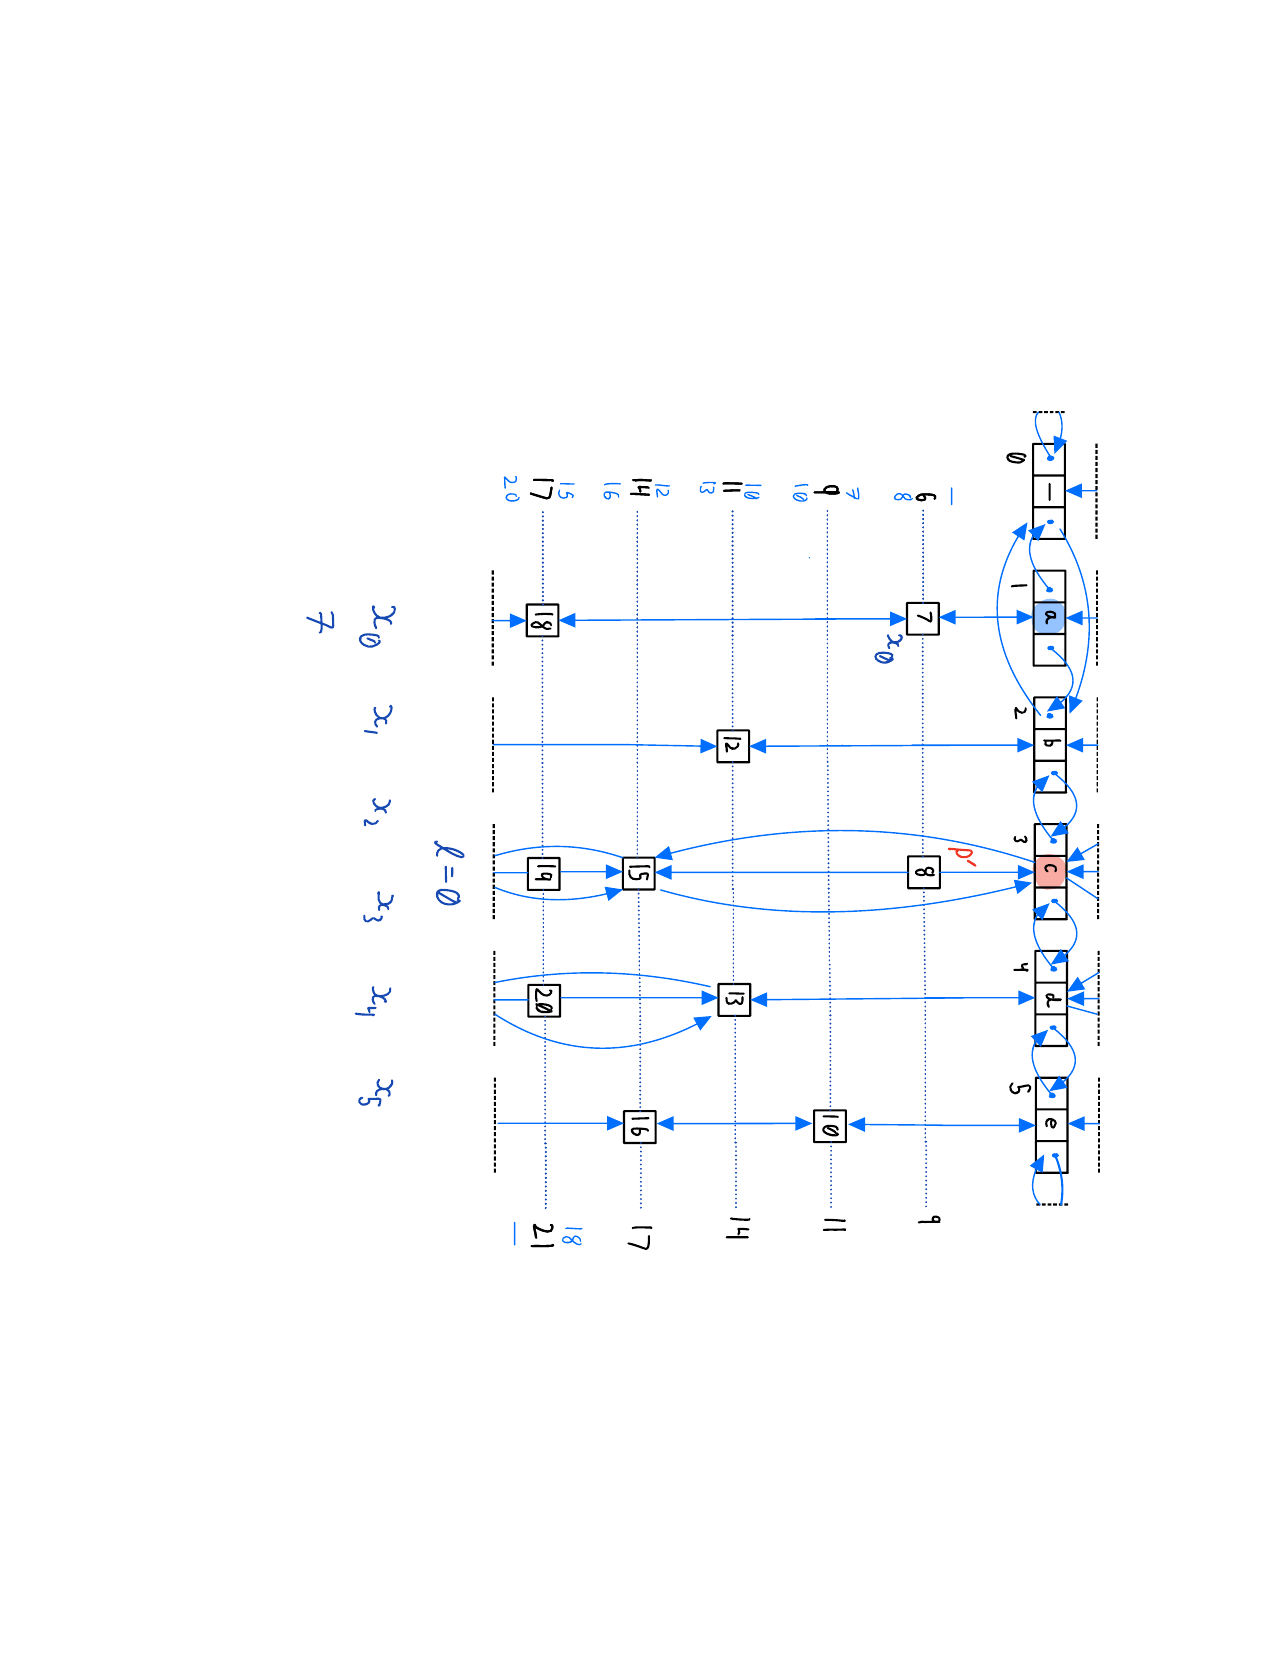
\includegraphics[angle=90,origin=c,scale=0.525]{images/Algorithm_X-19.png}} 
\begin{frame}{}
    \vspace{-130pt}
    cover($c$)
\end{frame} 
}

{ 
\usebackgroundtemplate{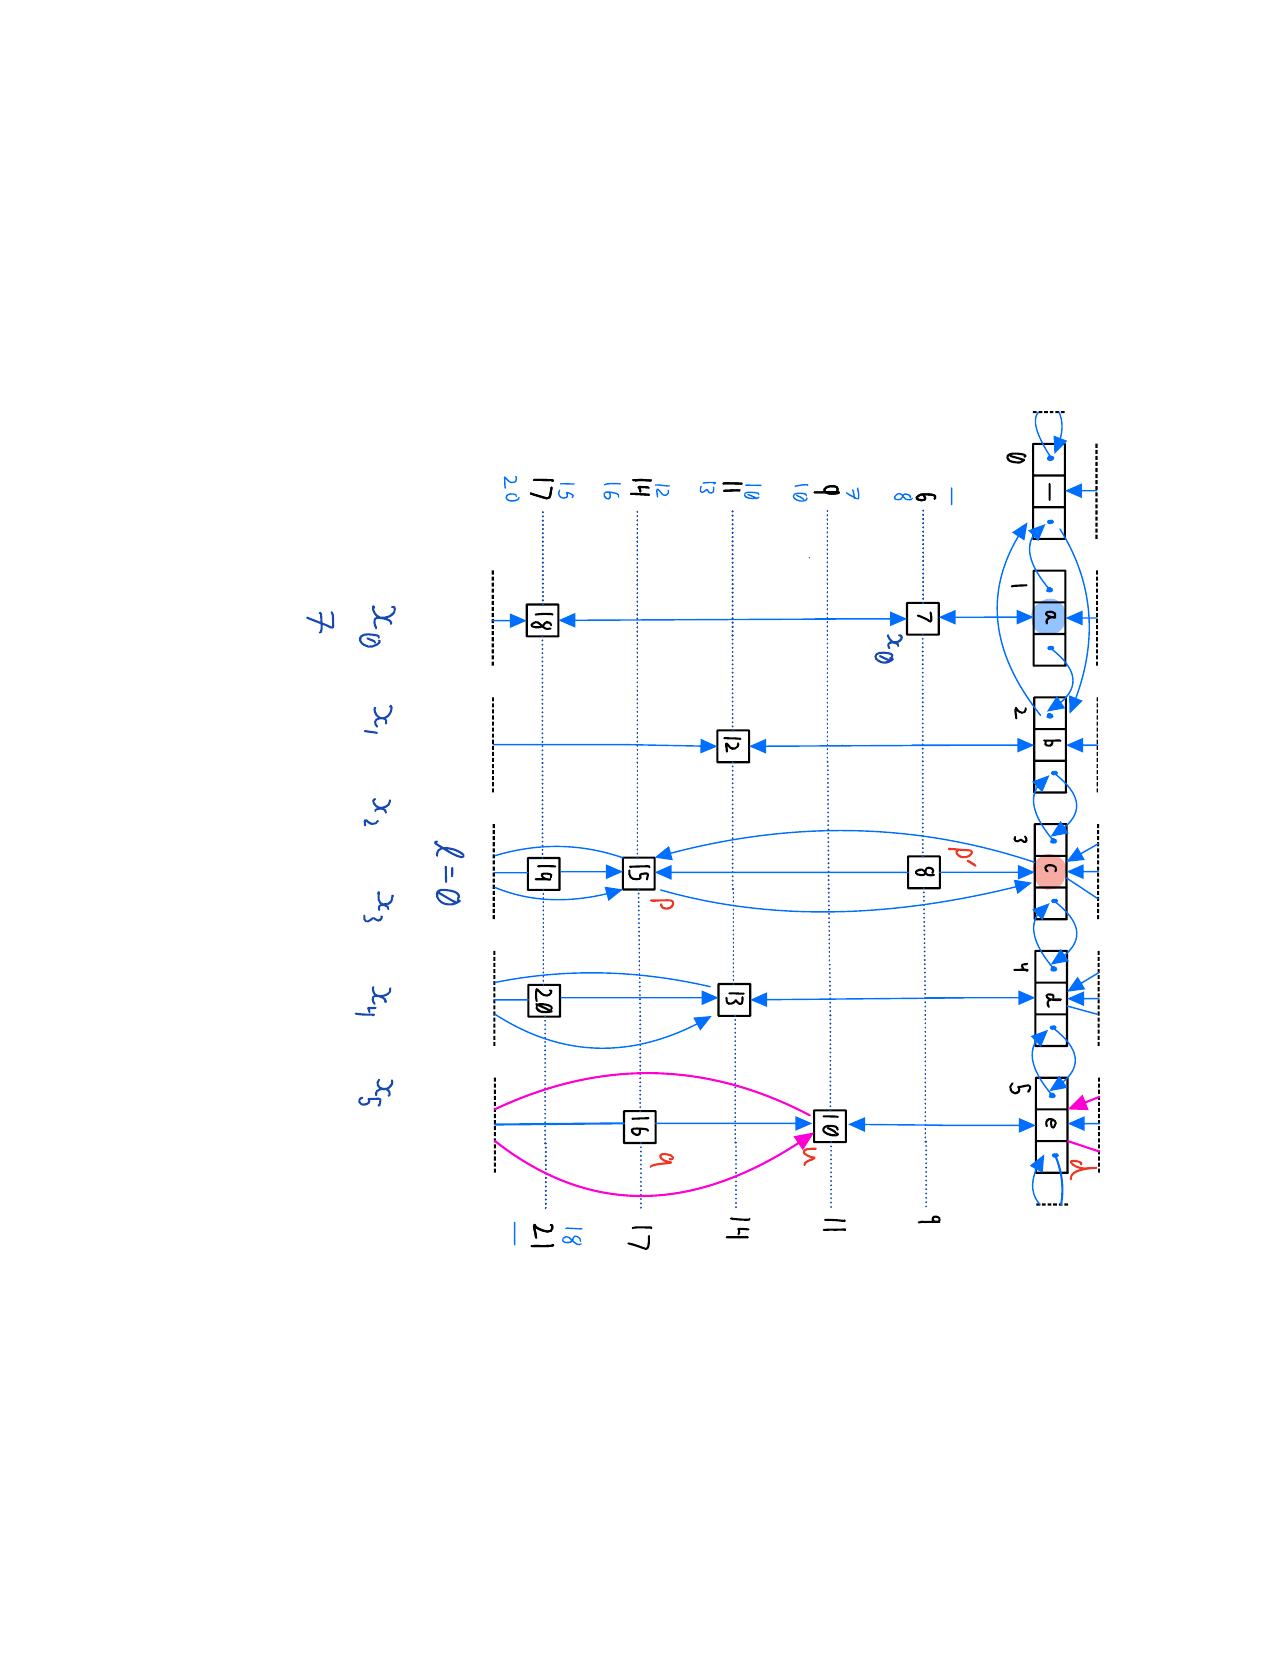
\includegraphics[angle=90,origin=c,scale=0.525]{images/Algorithm_X-20.png}} 
\begin{frame}{}
    \vspace{-130pt}
    hide($15$)
\end{frame} 
}

{ 
\usebackgroundtemplate{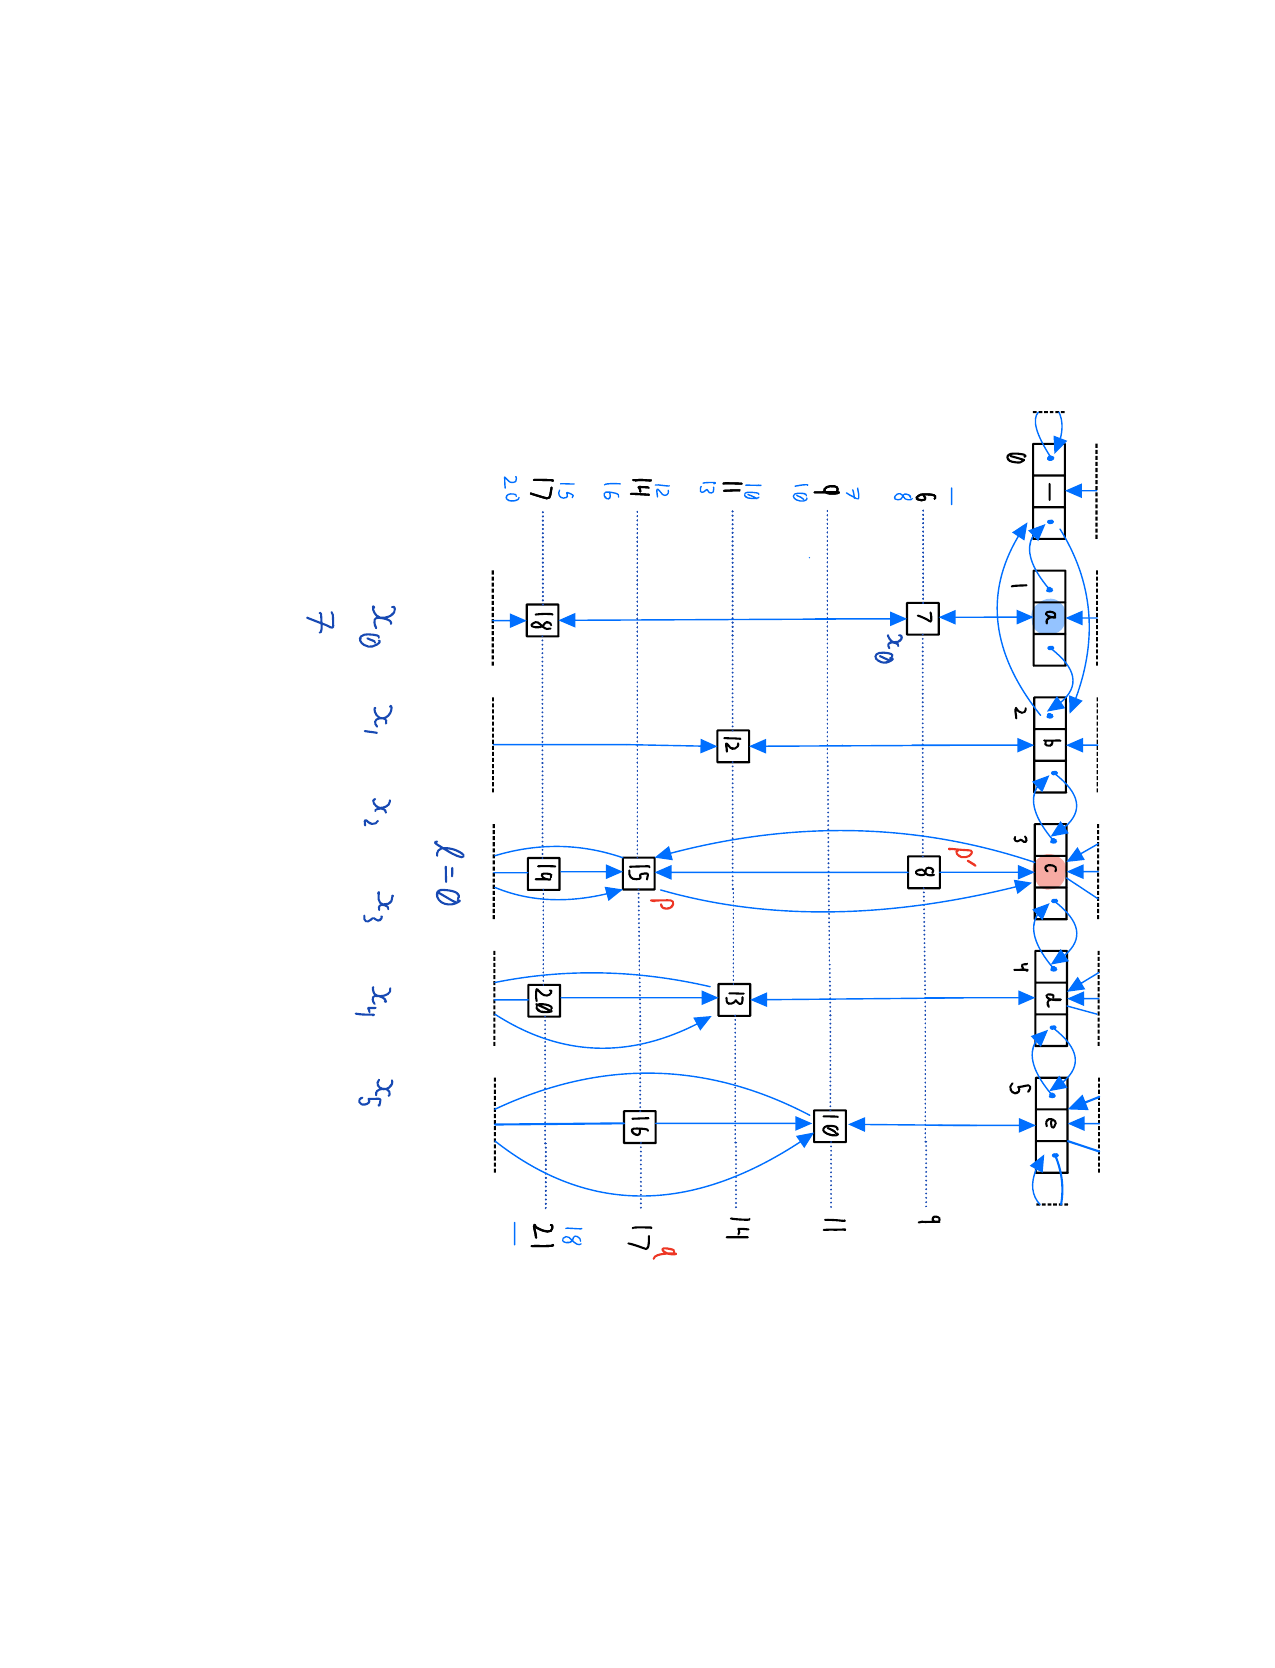
\includegraphics[angle=90,origin=c,scale=0.525]{images/Algorithm_X-21.png}} 
\begin{frame}{}
    \vspace{-130pt}
    hide($15$)
\end{frame} 
}

{ 
\usebackgroundtemplate{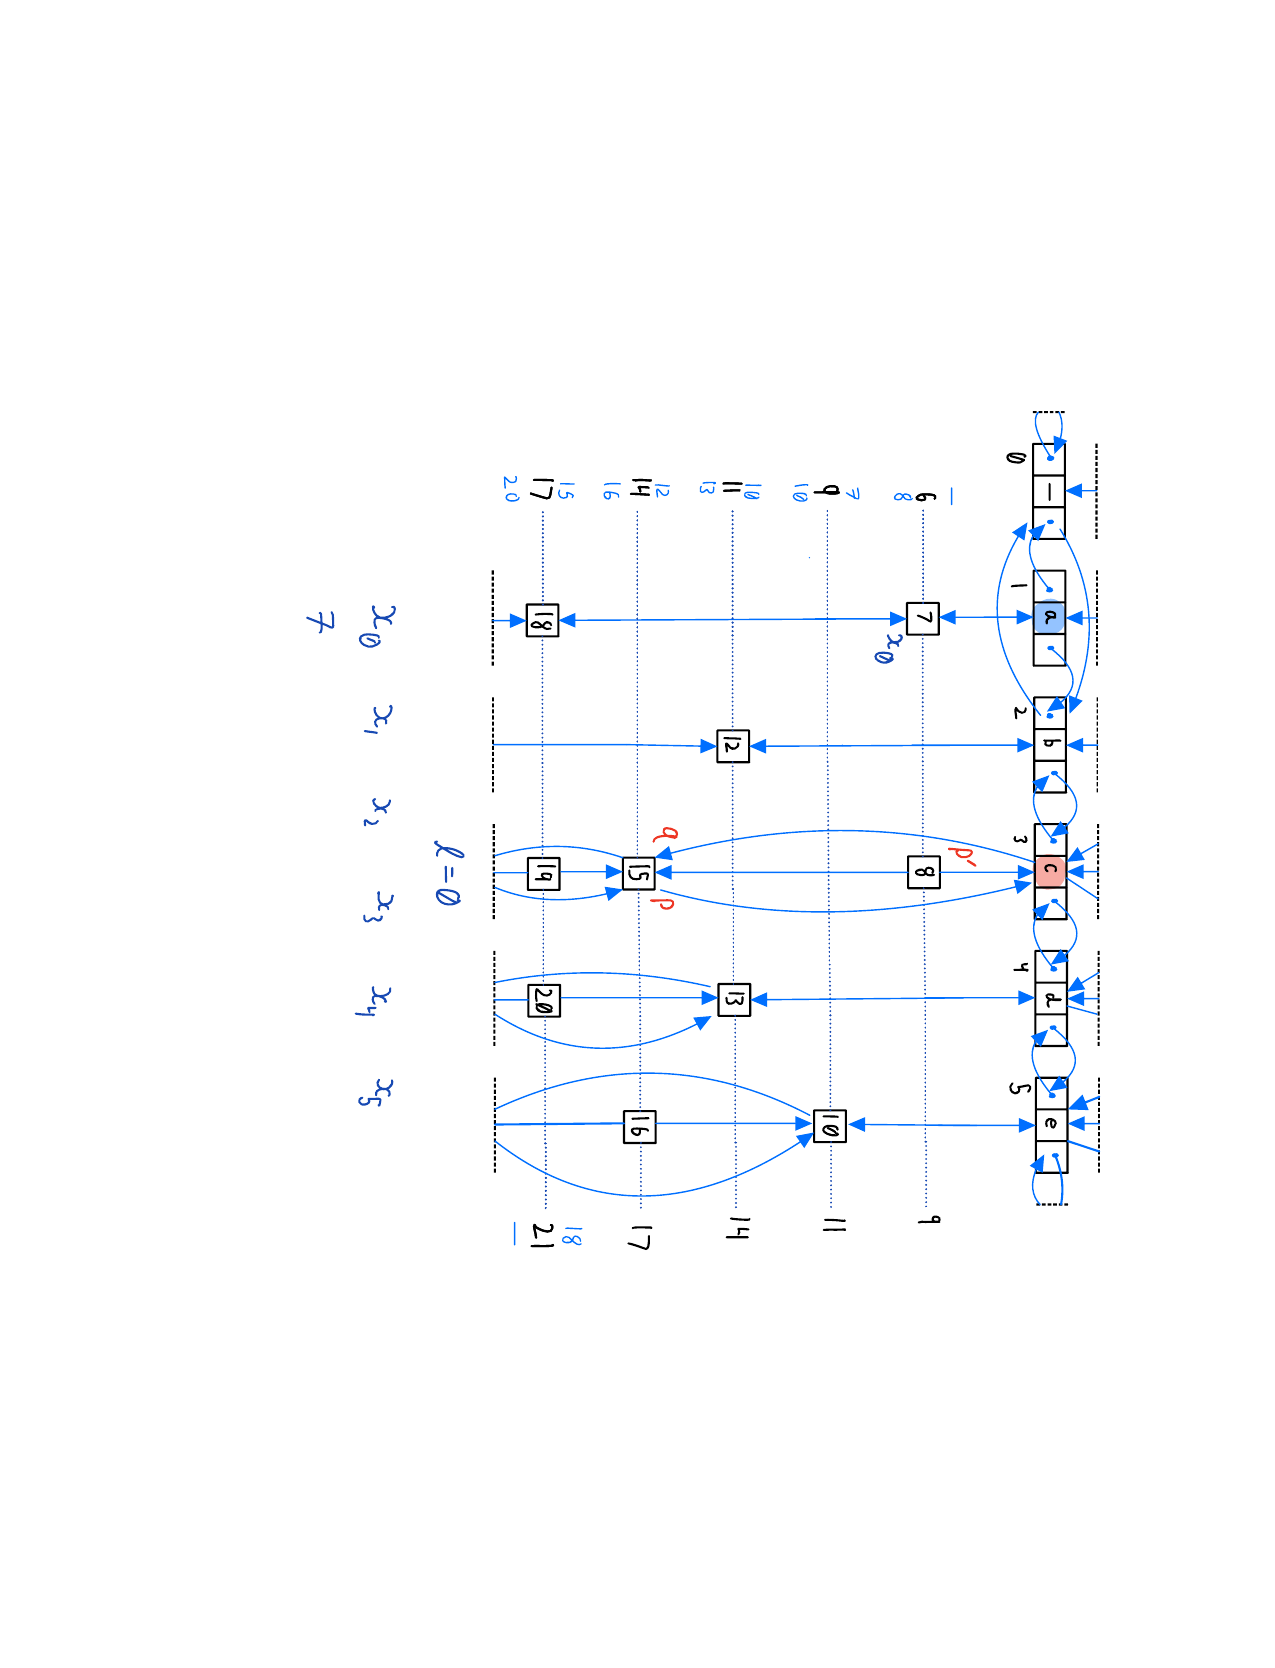
\includegraphics[angle=90,origin=c,scale=0.525]{images/Algorithm_X-22.png}} 
\begin{frame}{}
    \vspace{-130pt}
    hide($15$)
\end{frame} 
}

{ 
\usebackgroundtemplate{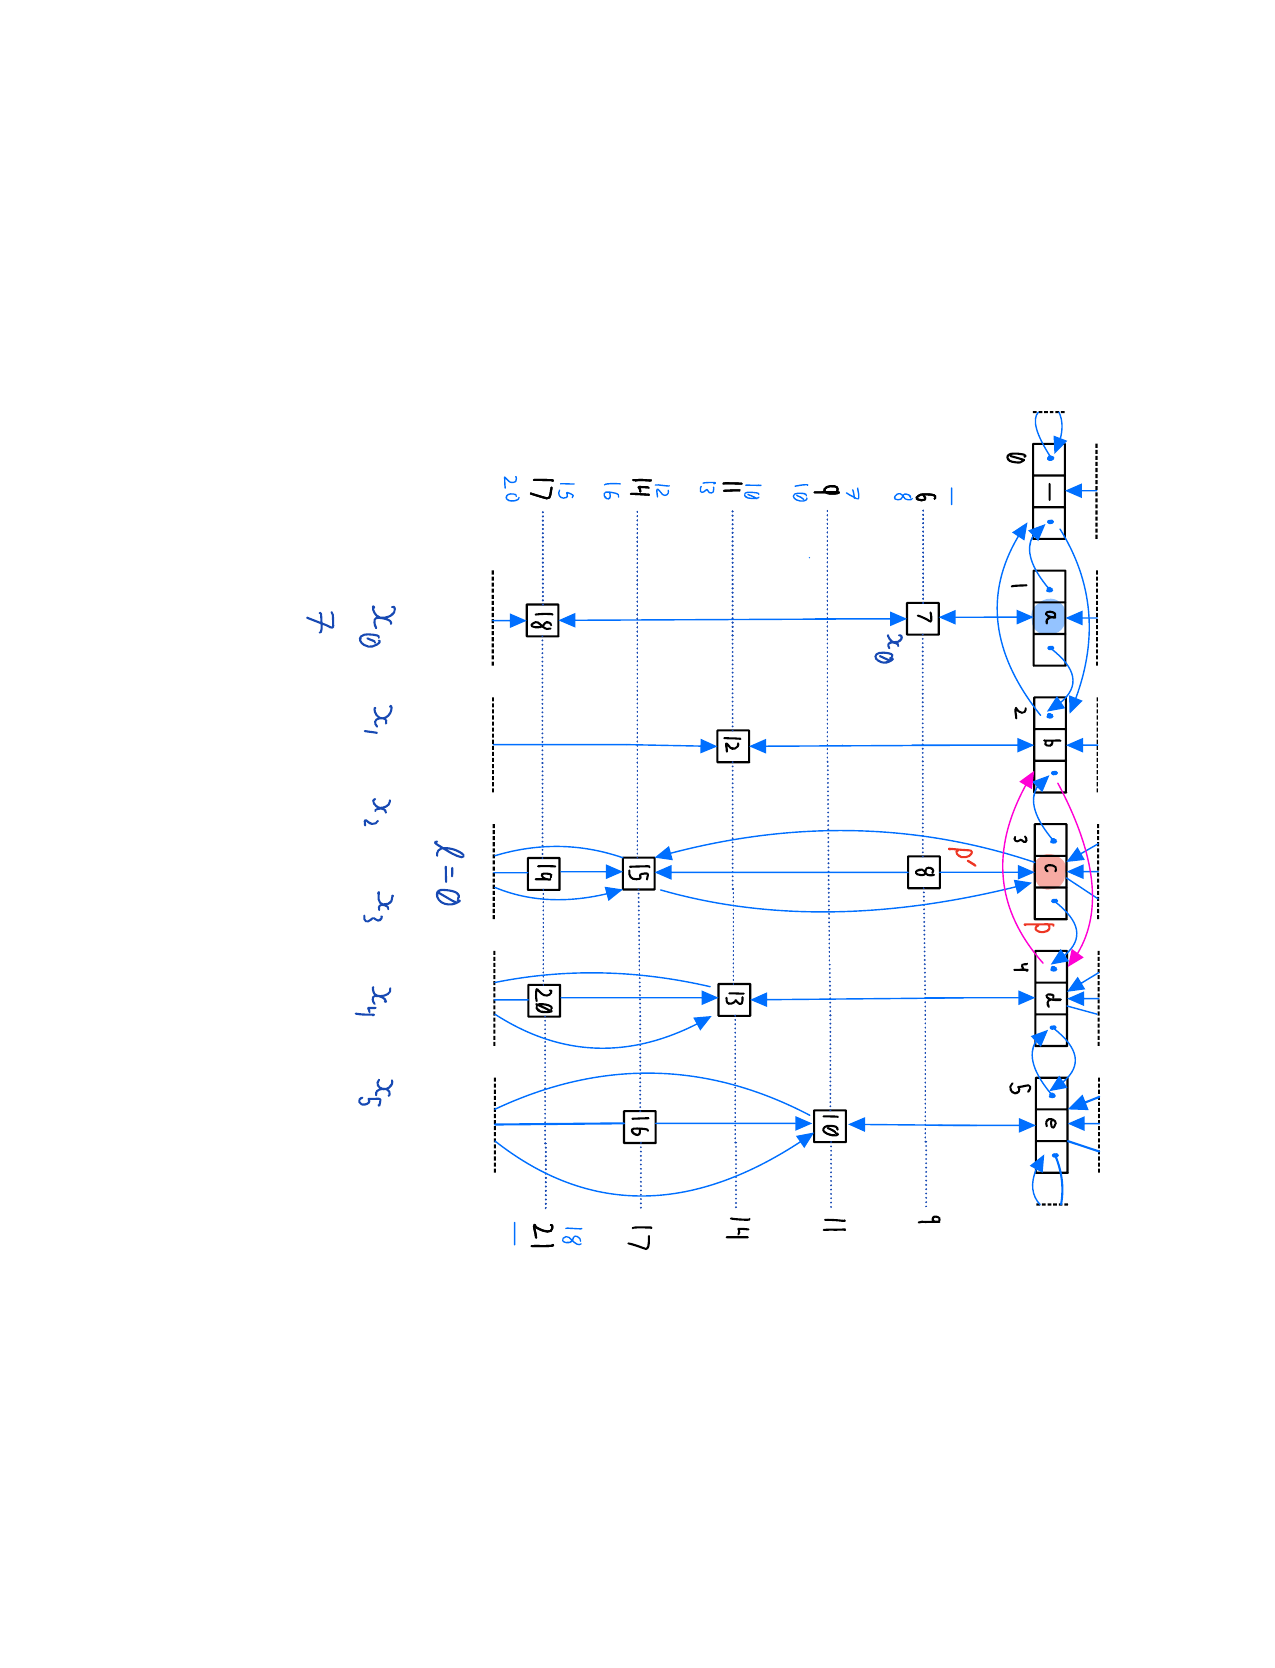
\includegraphics[angle=90,origin=c,scale=0.525]{images/Algorithm_X-23.png}} 
\begin{frame}{}
    \vspace{-130pt}
    remove $c$
\end{frame} 
}

{ 
\usebackgroundtemplate{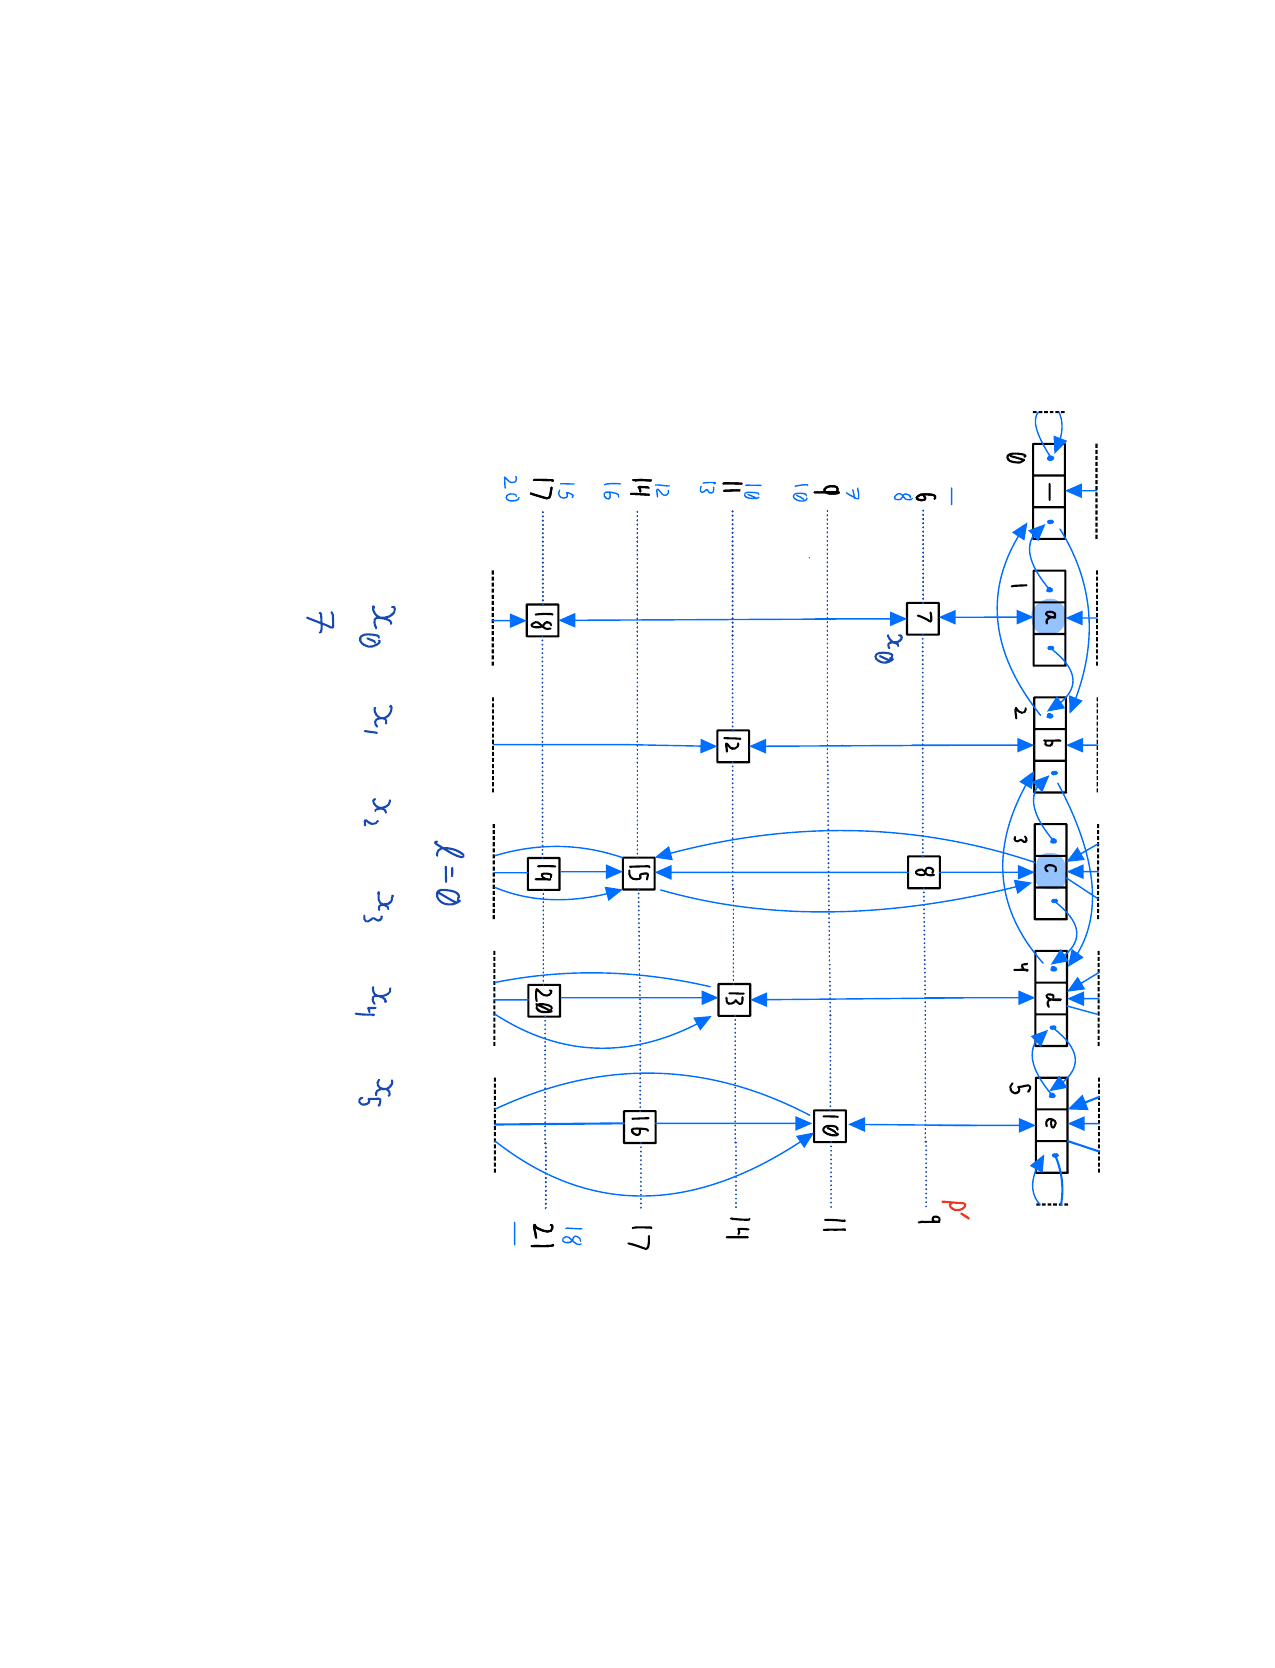
\includegraphics[angle=90,origin=c,scale=0.525]{images/Algorithm_X-24.png}} 
\begin{frame}{}
    \vspace{-130pt}
    $9$ is a spacer, go back to $7$
\end{frame} 
}

{ 
\usebackgroundtemplate{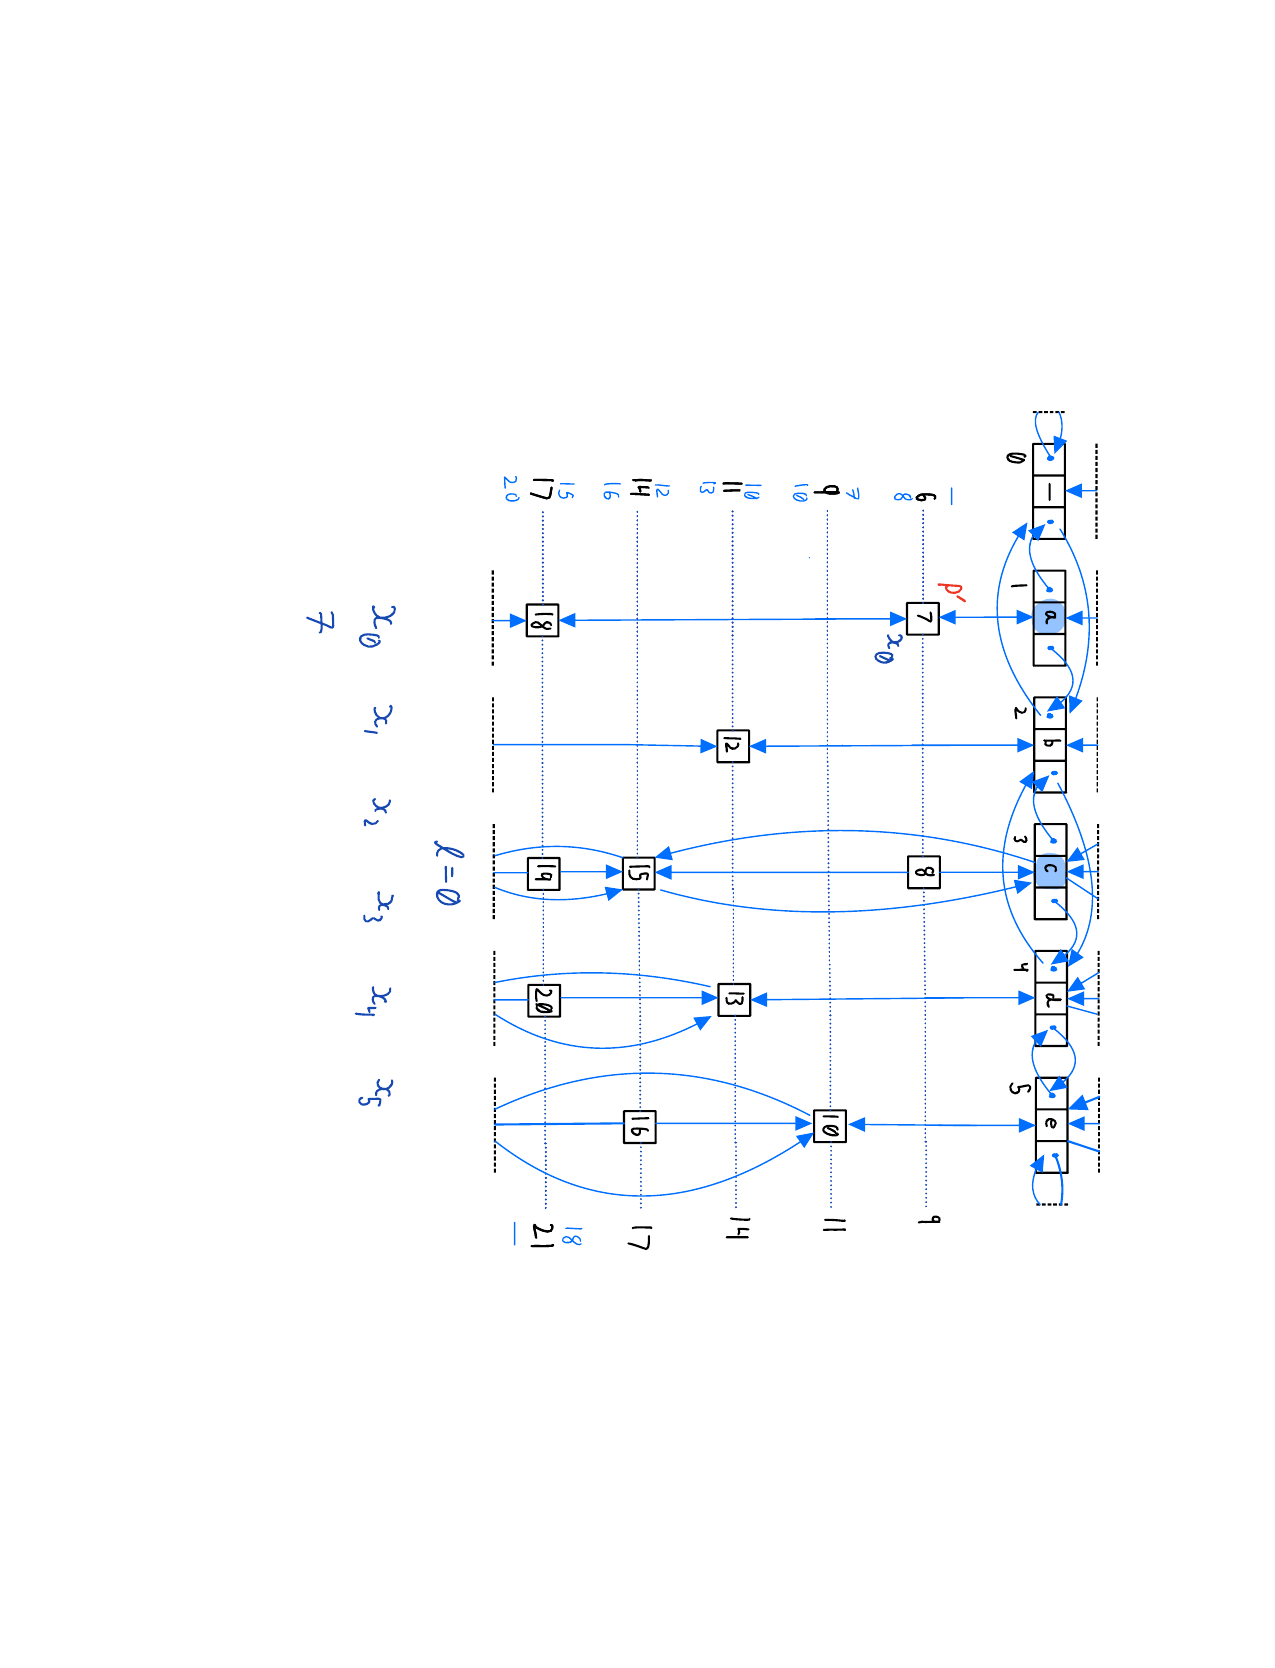
\includegraphics[angle=90,origin=c,scale=0.525]{images/Algorithm_X-25.png}} 
\begin{frame}{}
    \vspace{-130pt}
    $9$ is a spacer, go back to $7$
\end{frame} 
}

{ 
\usebackgroundtemplate{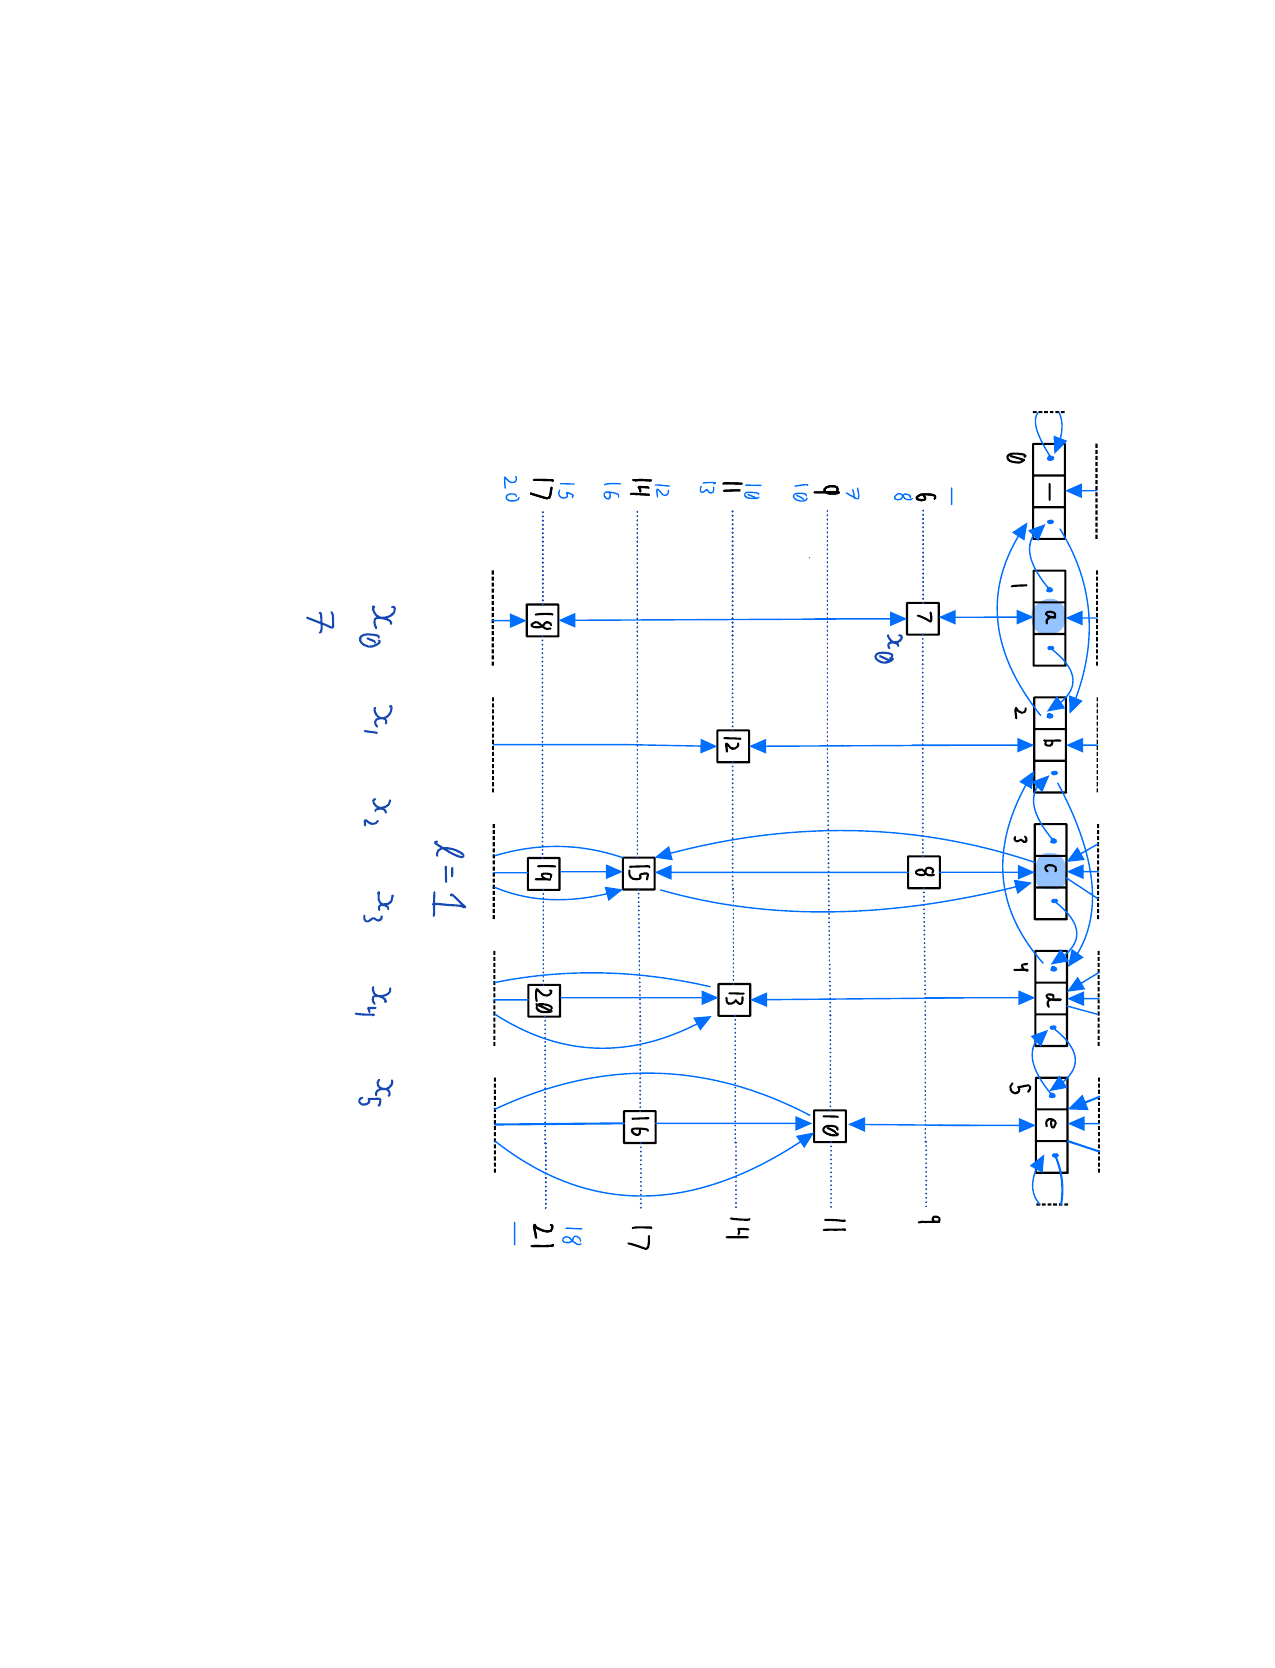
\includegraphics[angle=90,origin=c,scale=0.525]{images/Algorithm_X-26.png}} 
\begin{frame}{}
    \vspace{-130pt}
    $\ell=1$, attempt to cover $b$
\end{frame} 
}

{ 
\usebackgroundtemplate{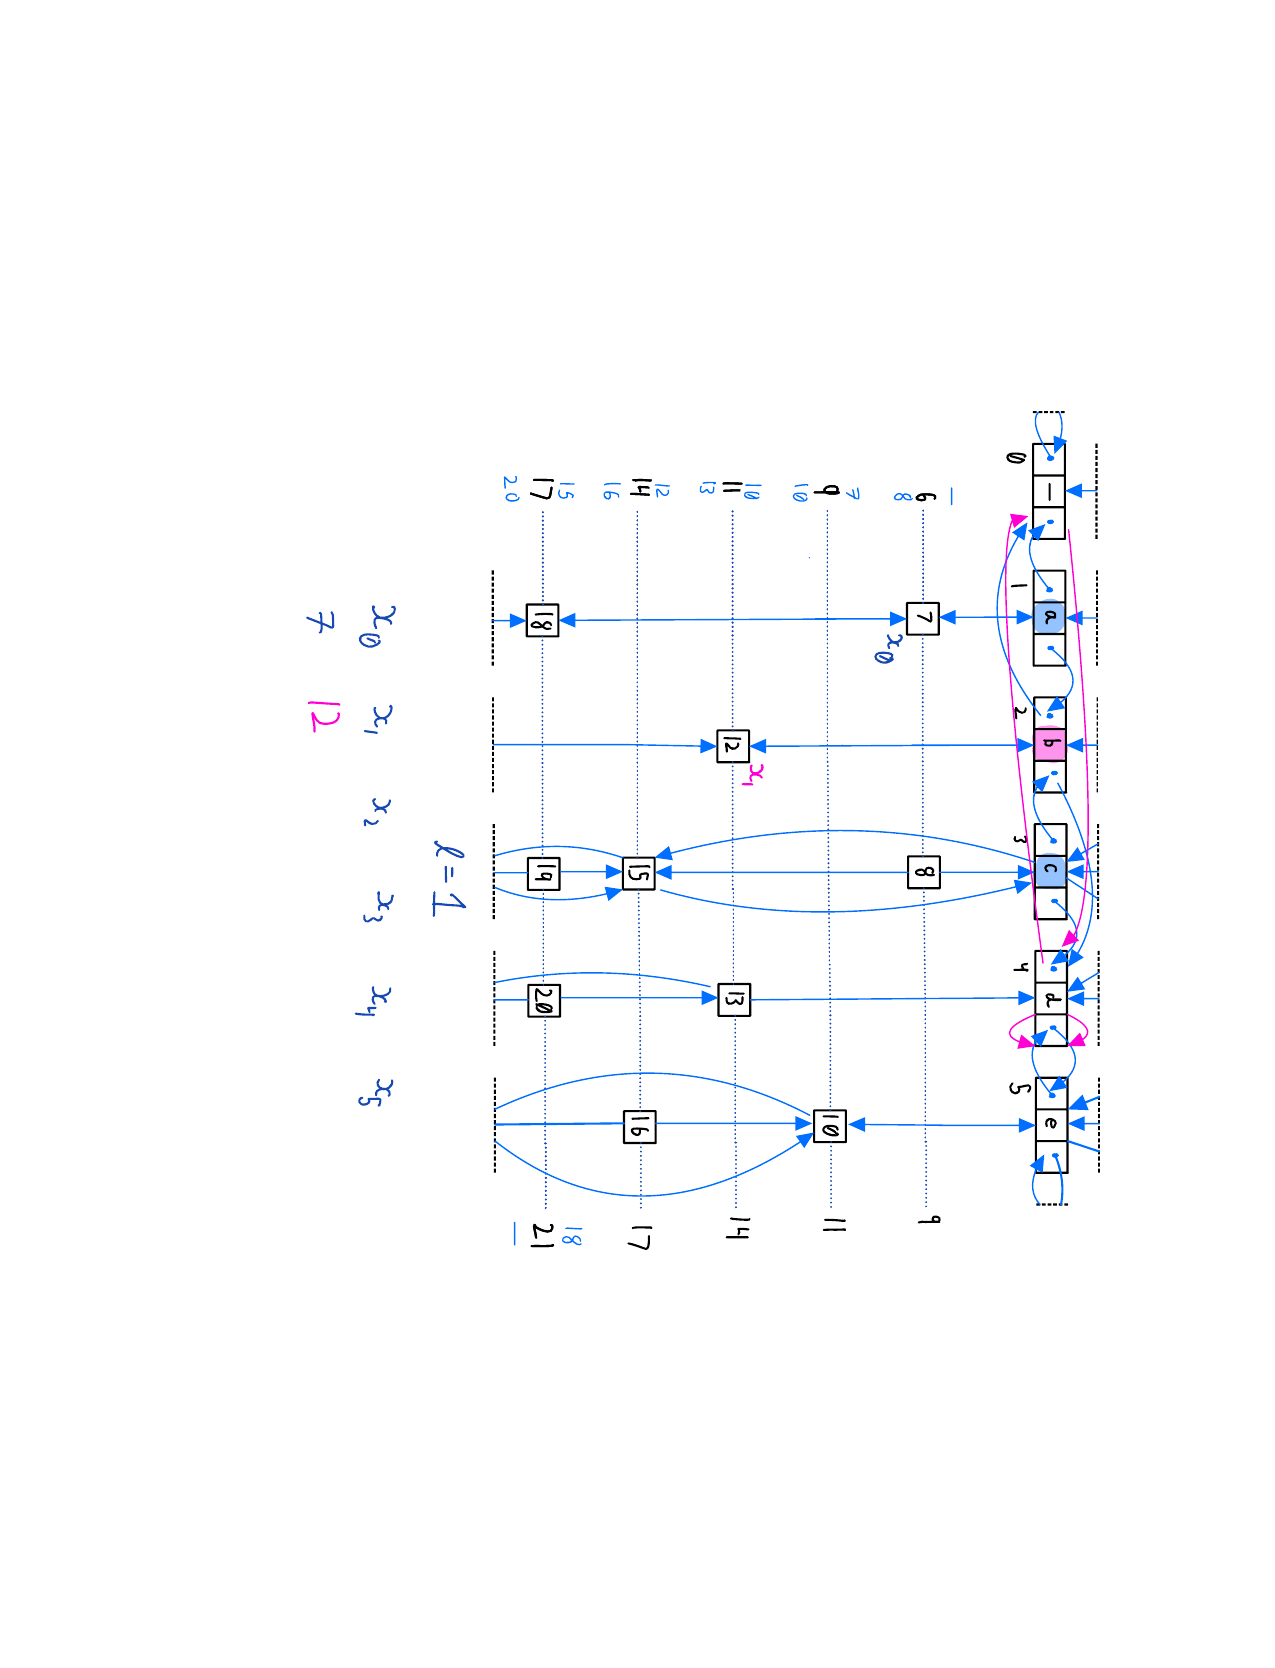
\includegraphics[angle=90,origin=c,scale=0.525]{images/Algorithm_X-27.png}} 
\begin{frame}{}
    \vspace{-130pt}
    $\ell=1$, attempt to cover $b$
\end{frame} 
}

{ 
\usebackgroundtemplate{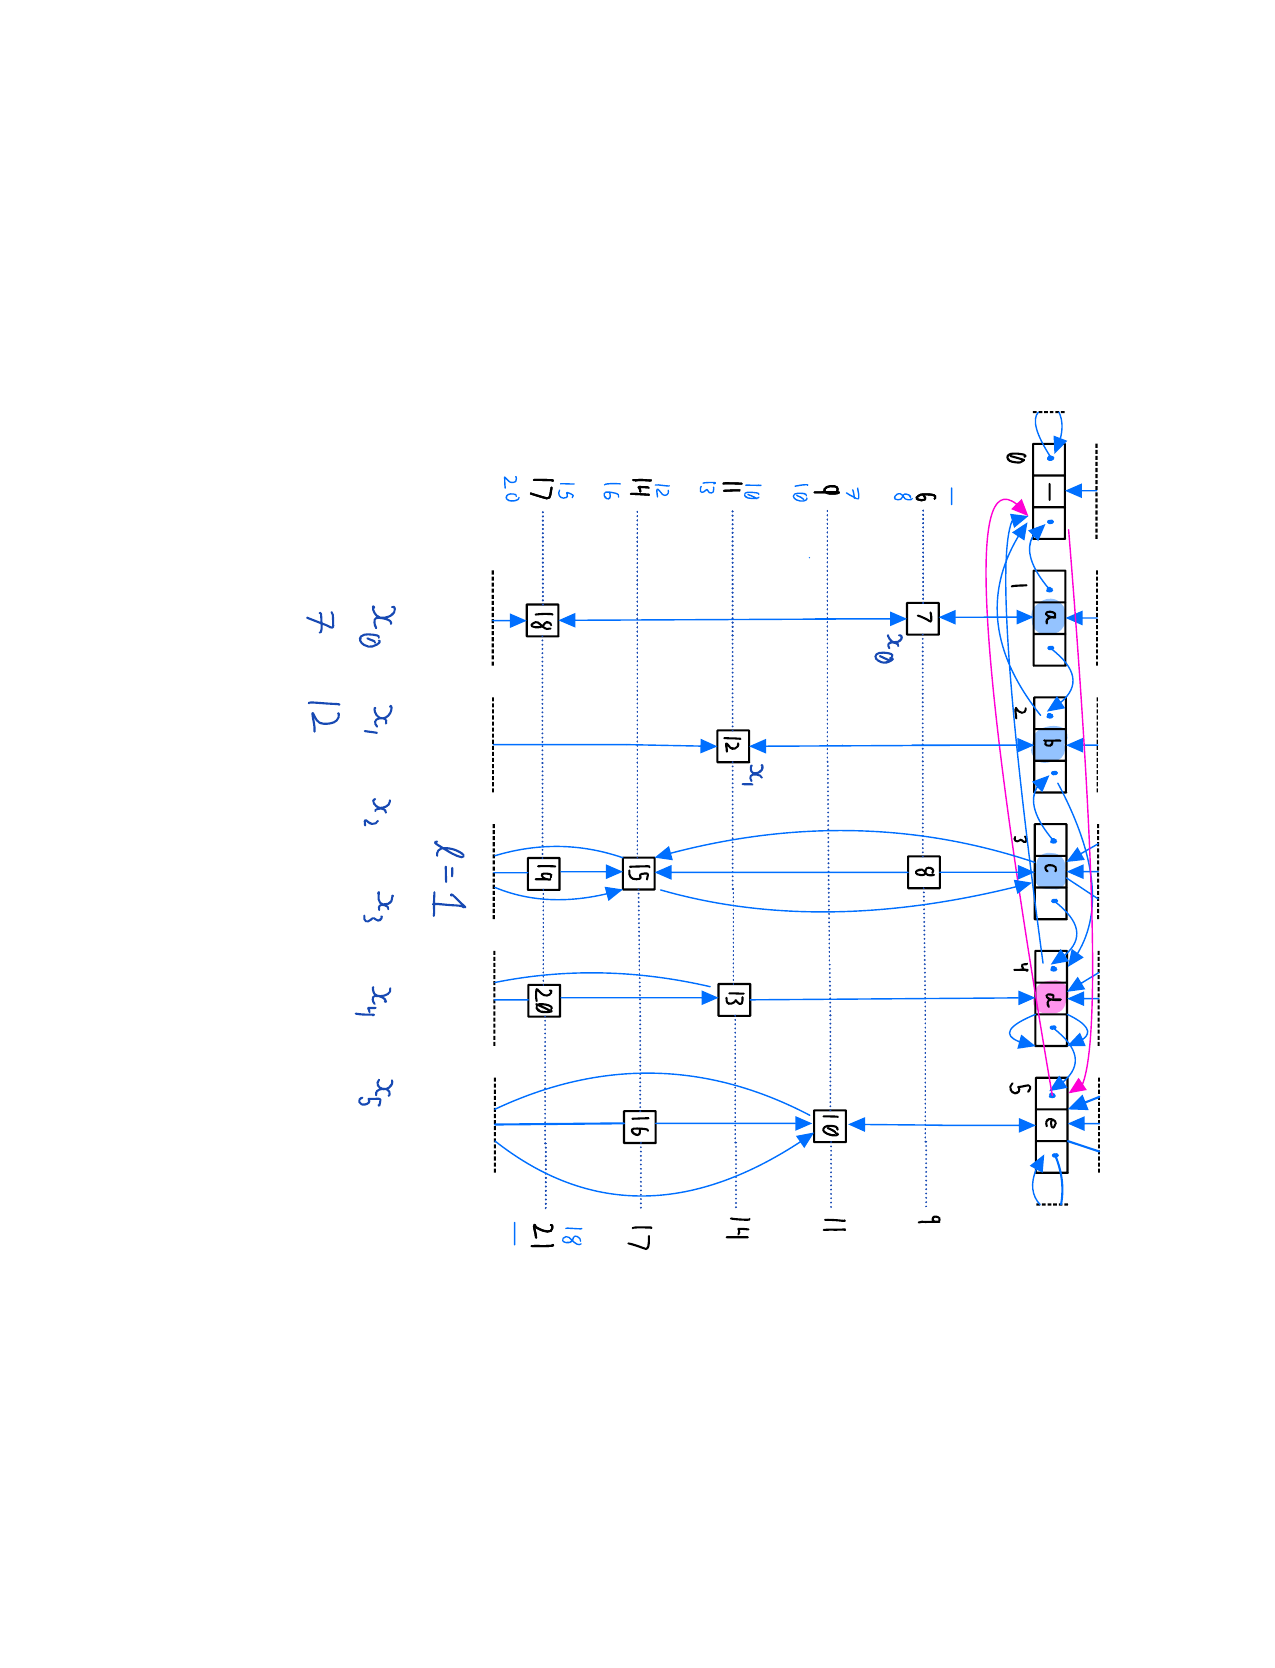
\includegraphics[angle=90,origin=c,scale=0.525]{images/Algorithm_X-28.png}} 
\begin{frame}{}
    \vspace{-130pt}
    This option covers $d$ as well
\end{frame} 
}

{ 
\usebackgroundtemplate{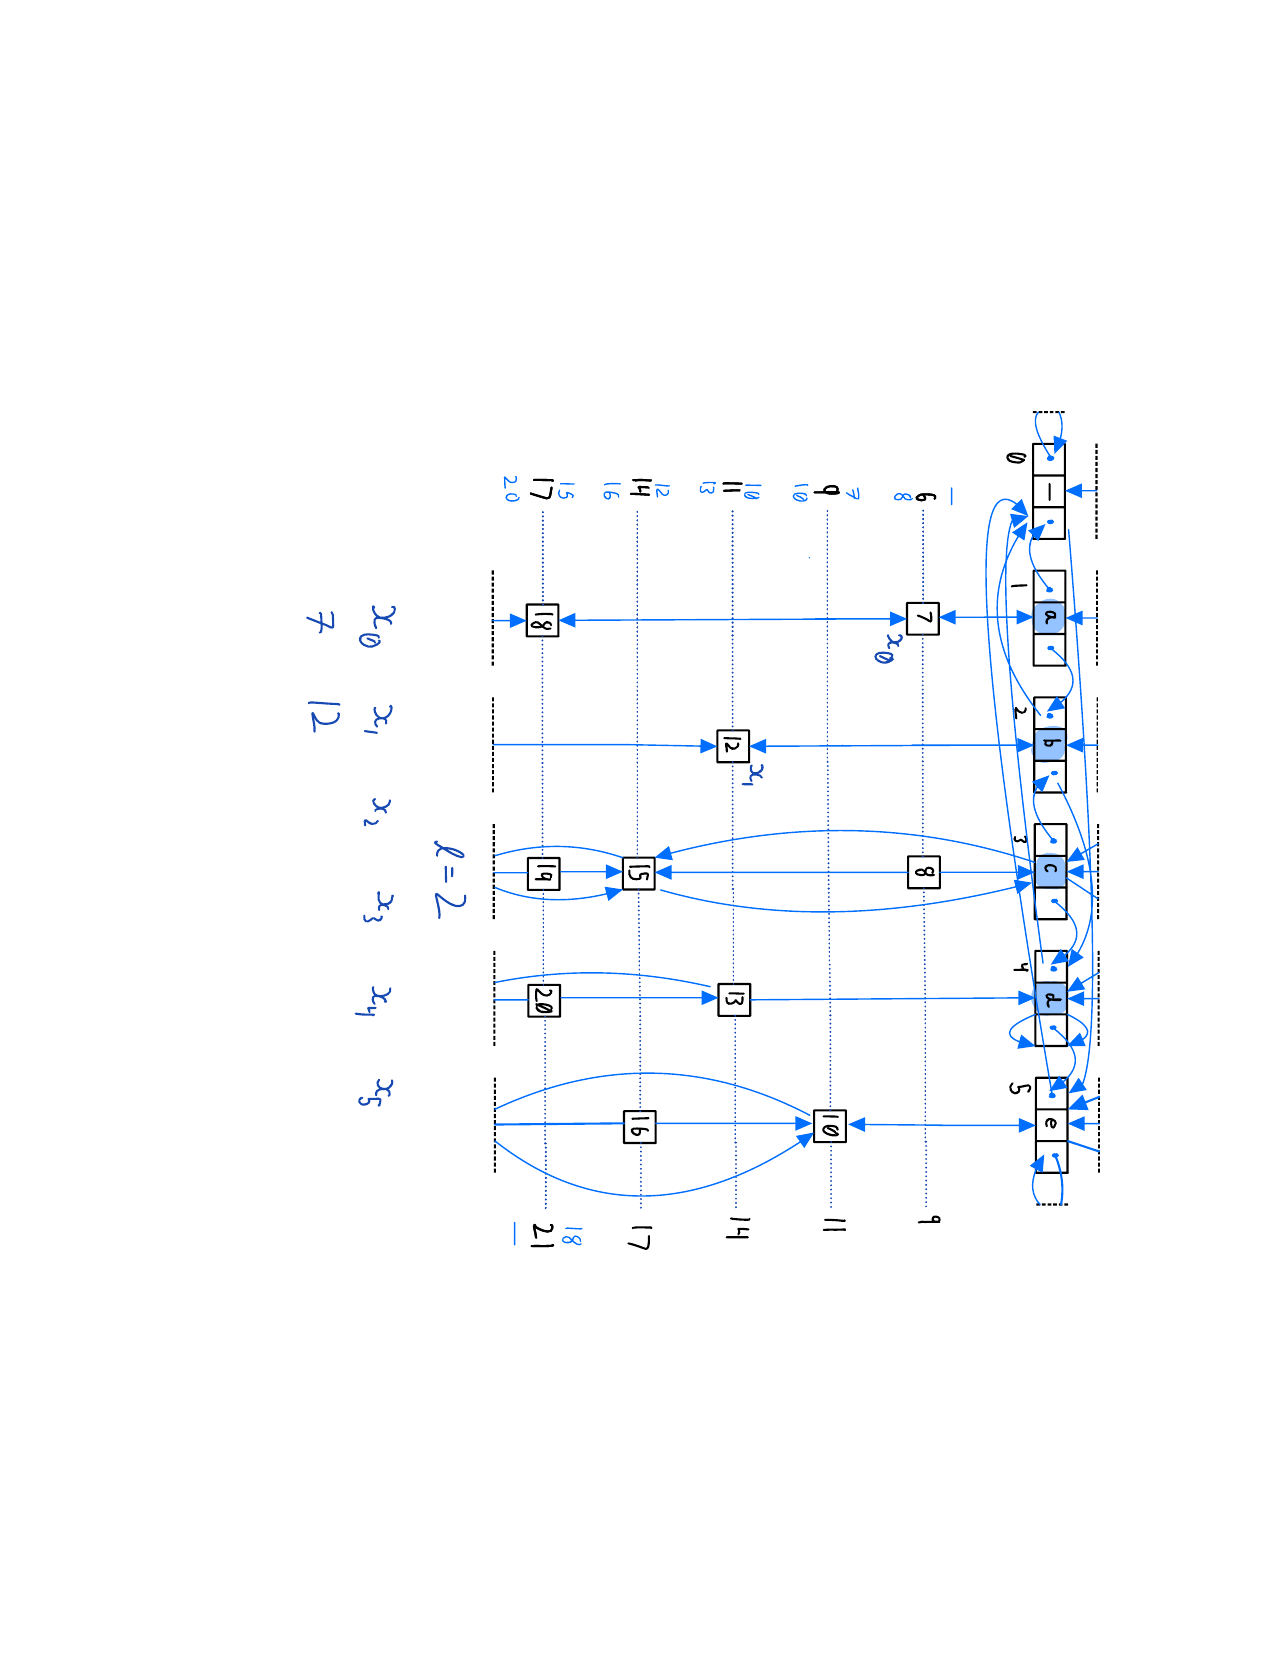
\includegraphics[angle=90,origin=c,scale=0.525]{images/Algorithm_X-29.png}} 
\begin{frame}{}
    \vspace{-130pt}
    Only remaining item is $e$
\end{frame} 
}

{ 
\usebackgroundtemplate{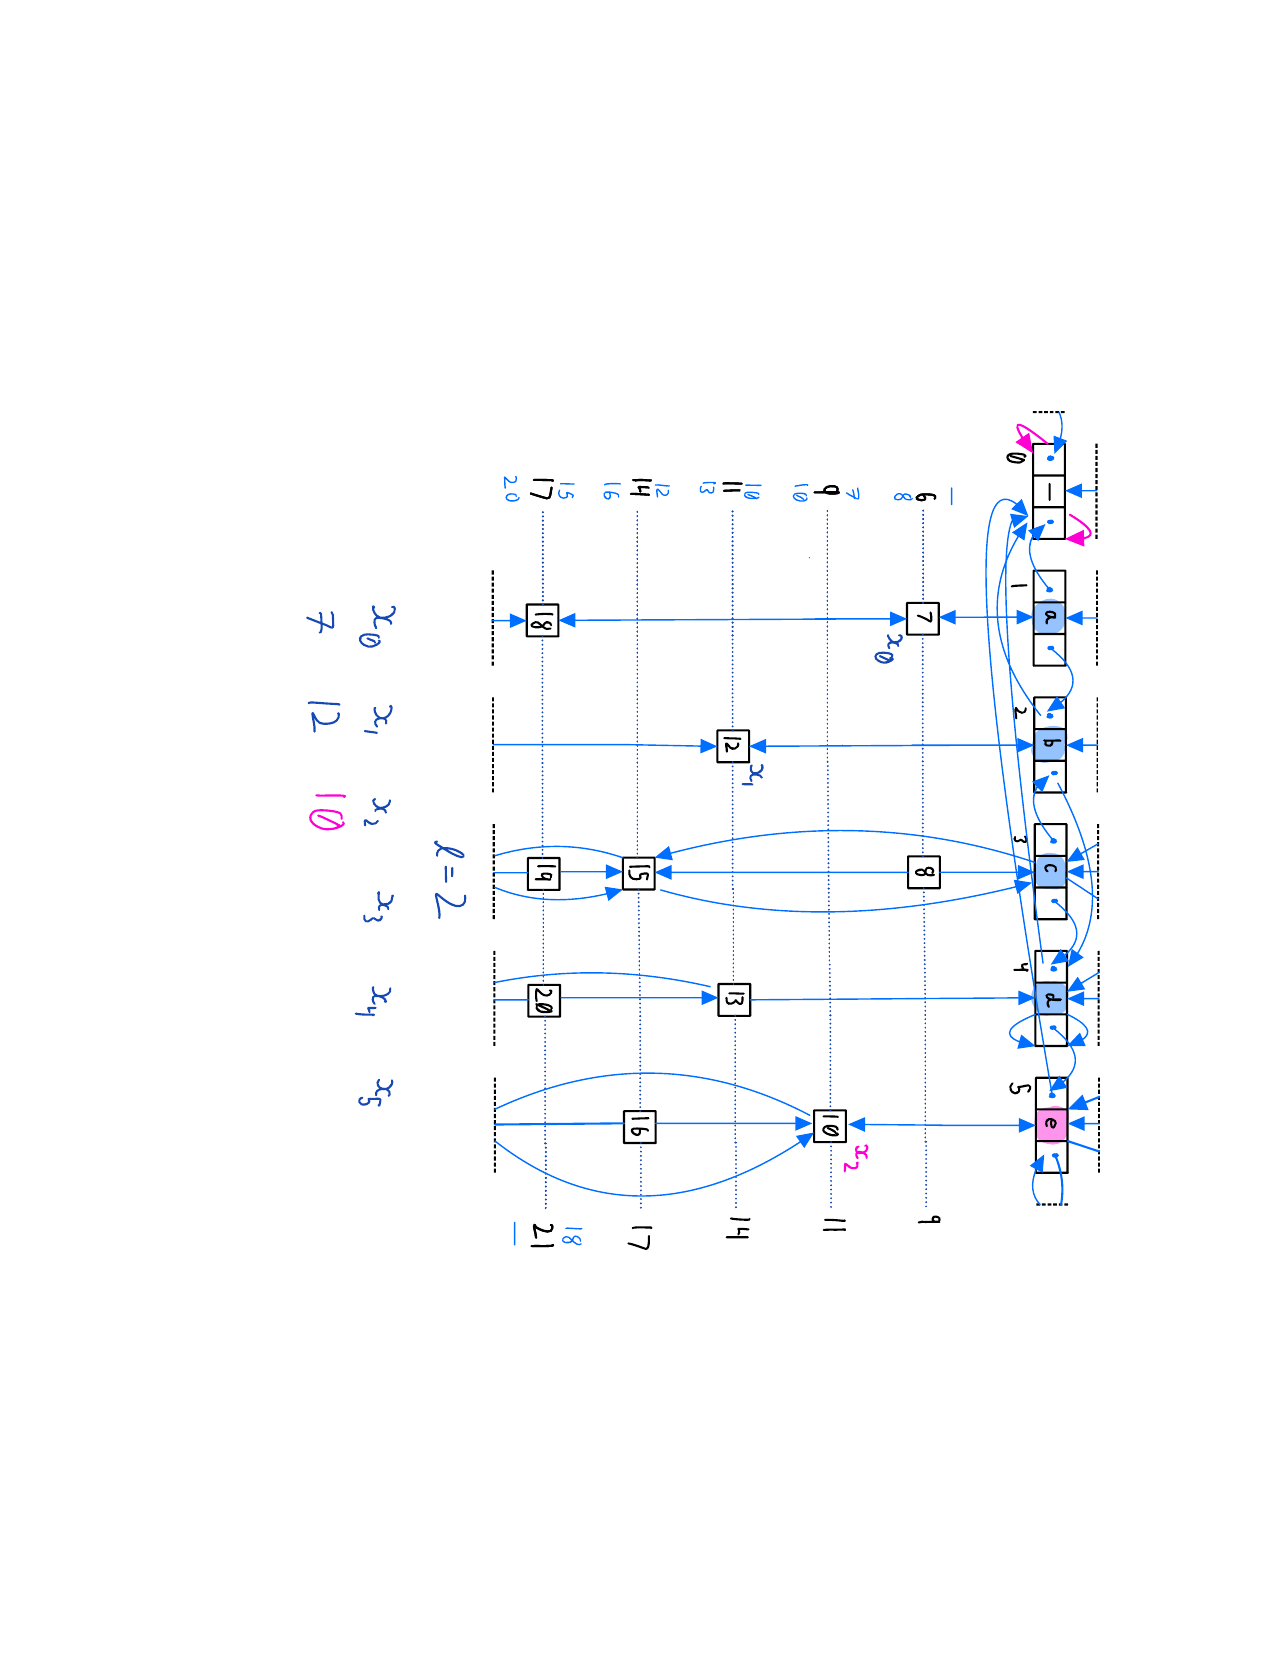
\includegraphics[angle=90,origin=c,scale=0.525]{images/Algorithm_X-30.png}} 
\begin{frame}{}
    \vspace{-130pt}
    cover($e$)
\end{frame} 
}

{ 
\usebackgroundtemplate{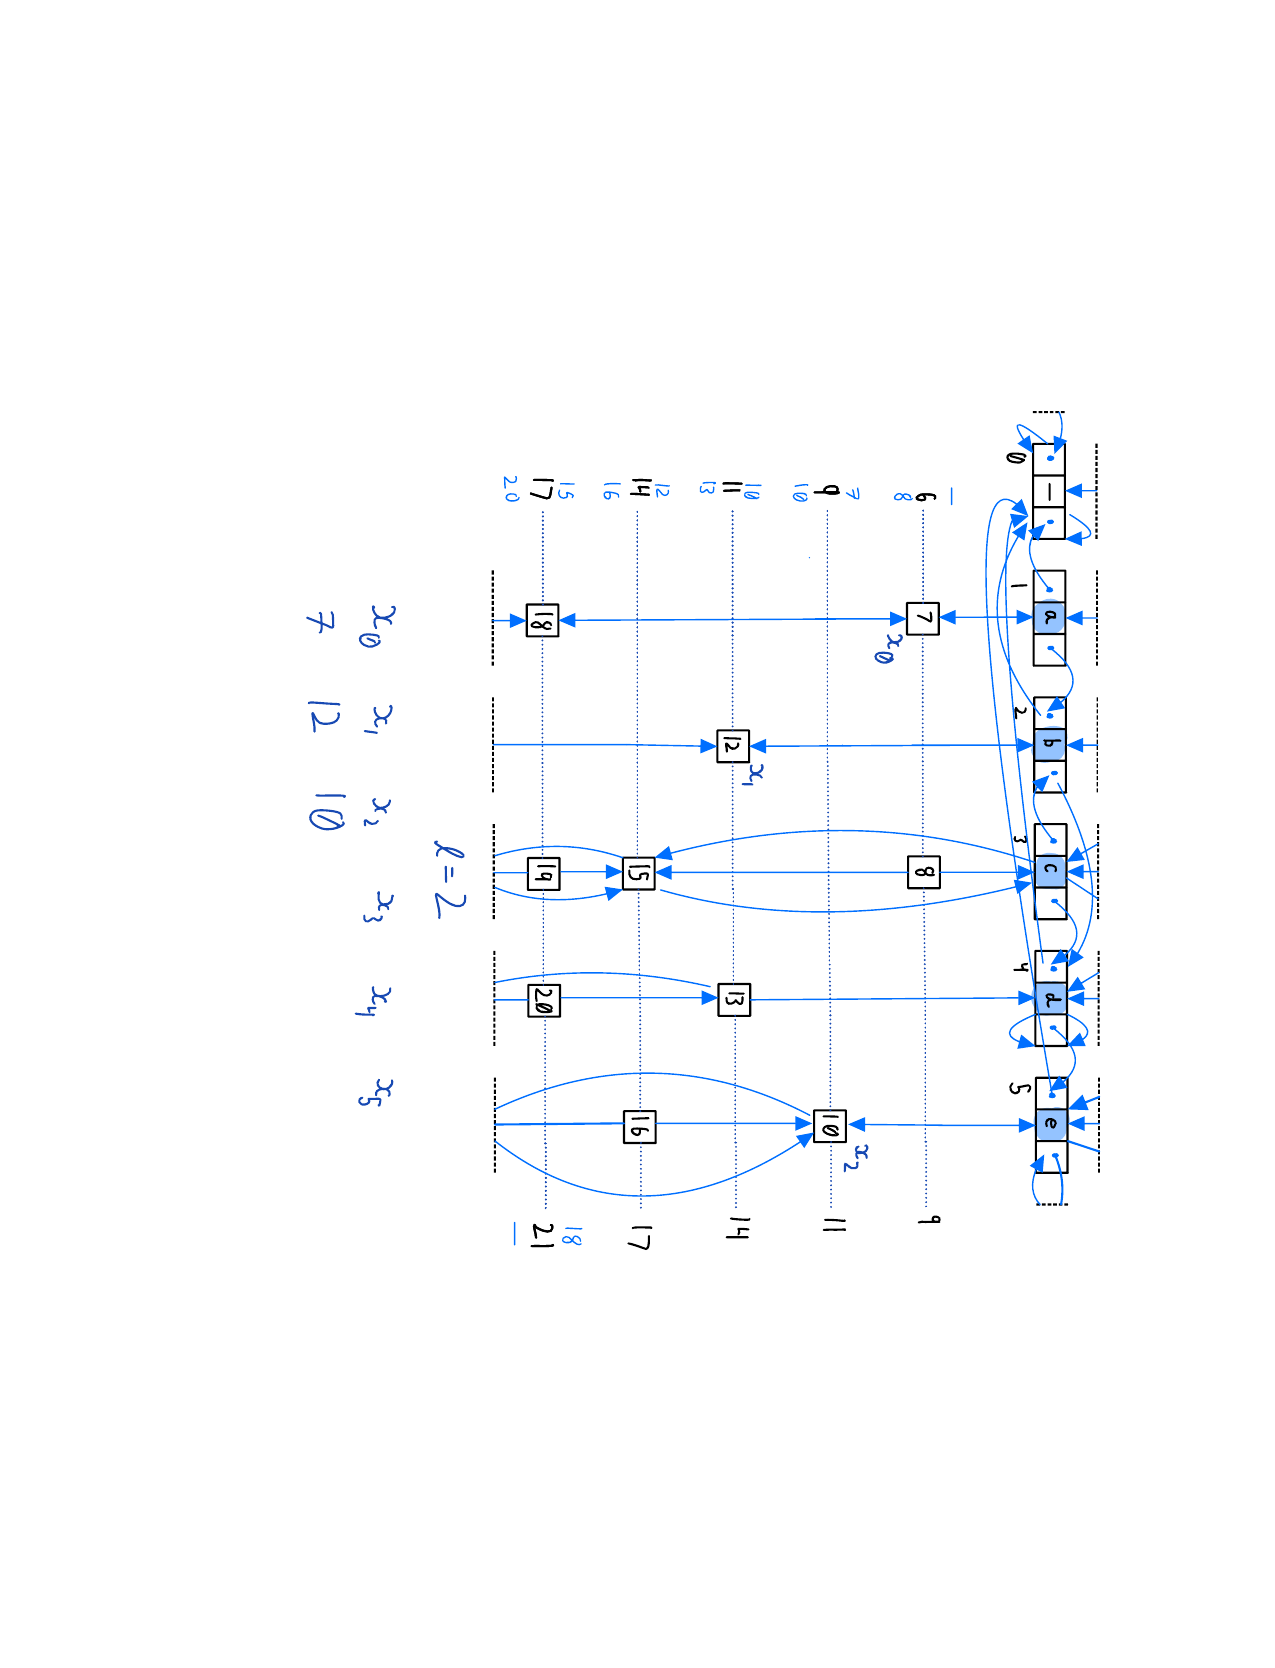
\includegraphics[angle=90,origin=c,scale=0.525]{images/Algorithm_X-31.png}} 
\begin{frame}{}
    \vspace{-130pt}
    cover($e$)
\end{frame} 
}

{ 
\usebackgroundtemplate{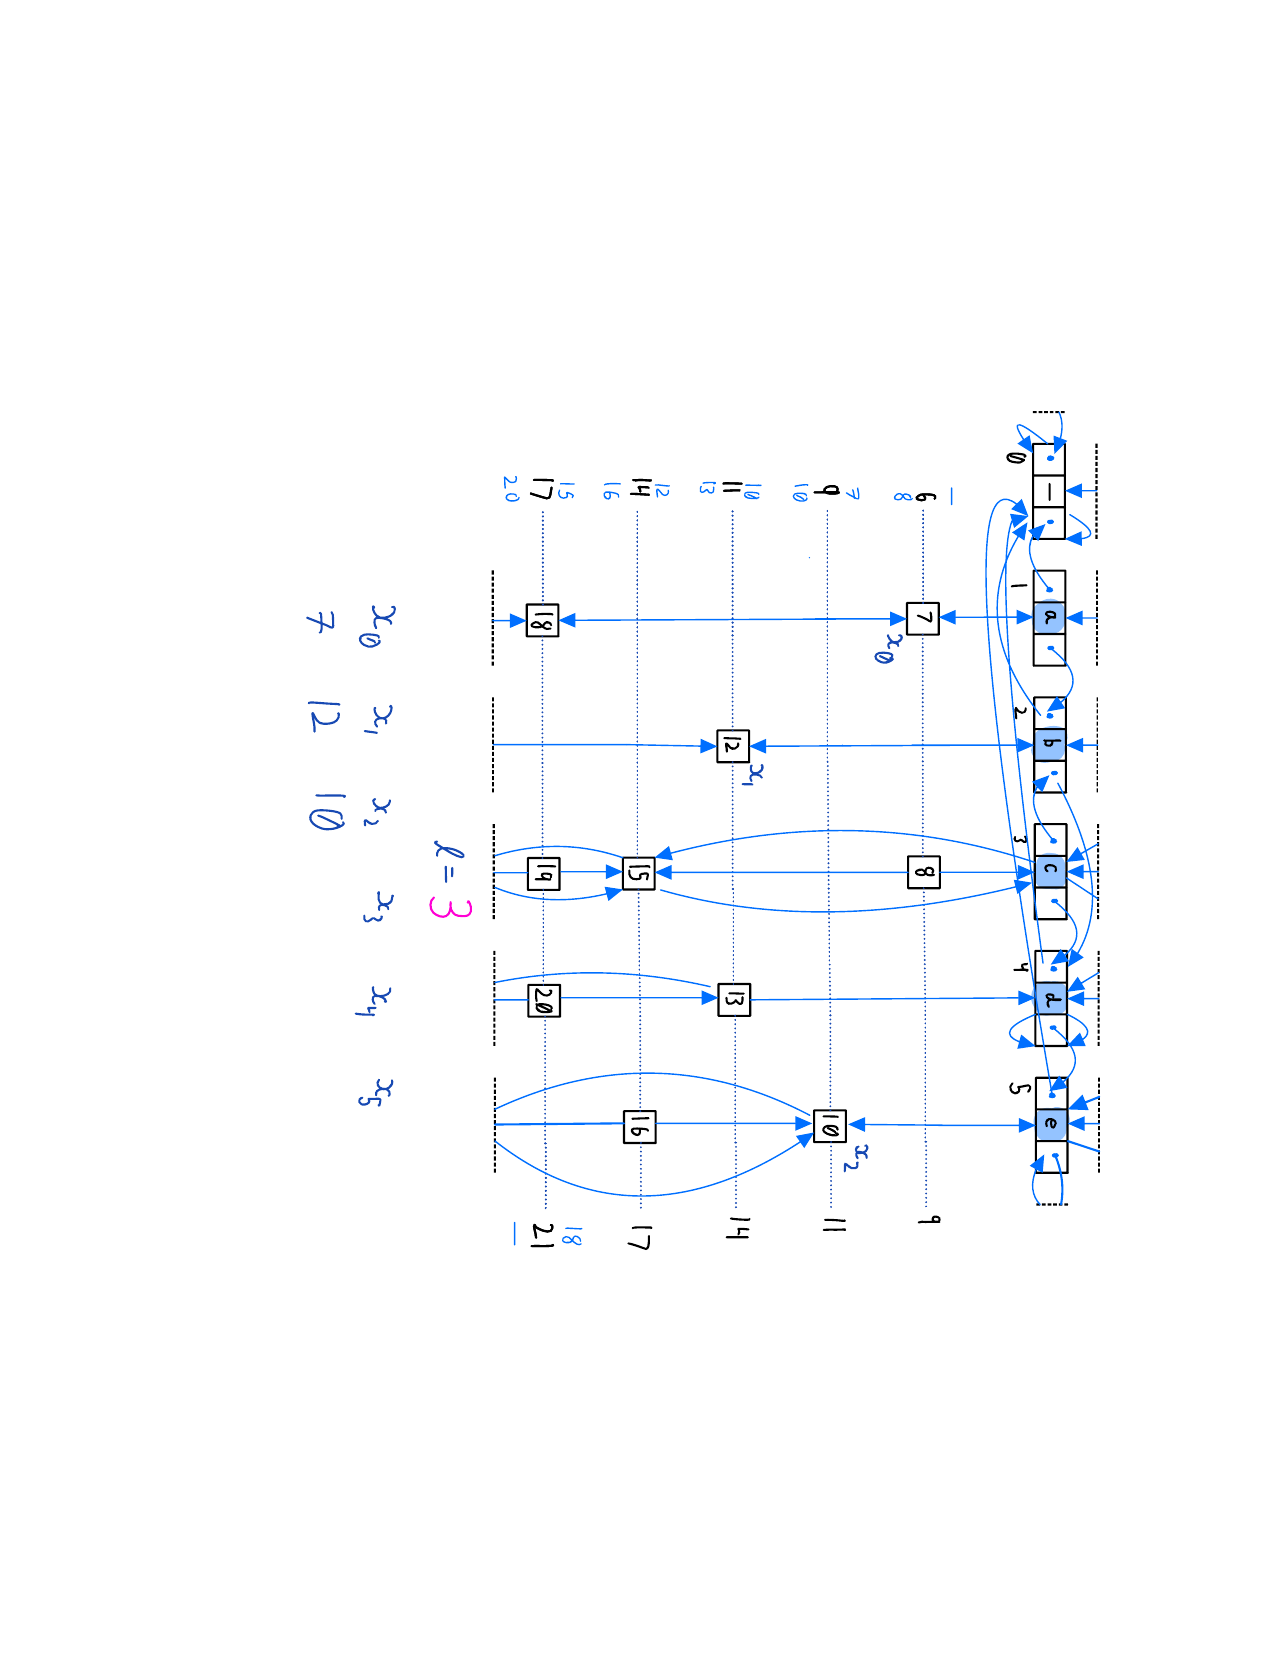
\includegraphics[angle=90,origin=c,scale=0.525]{images/Algorithm_X-32.png}} 
% \defbeamertemplate*{background}{blank}{} 
\begin{frame}{}
    \vspace{-130pt}
    No options left to cover
\end{frame} 
}

\begin{frame}{Recovering The Answer}
    \begin{itemize}
        \item Now our list contains links {\color{sigma@mainblue}$7$}, {\color{sigma@mainblue}$12$}, and {\color{sigma@mainblue}$10$}.
        \item How do we recover what options we selected? \pause
        \item Each node contains a field pointing to the corresponding option
        \begin{itemize}
            \item Data structure design is half the battle
        \end{itemize}
    \end{itemize}
\end{frame}


%have you ever wondered: what if a linked list was actually SEVERAL linked lists, all of which were circular and had both up, down, left, AND right links? :D


\begin{frame}{}
      \begin{center}
    {\color{sigma@mainblue} \LARGE Questions?}
  \end{center}
\end{frame}

% \font\eightss=cmssq8
% \font\eightssi=cmssqi8
% \newcommand\quoteAuthorDate[3]{\begingroup
%   \baselineskip 10pt
%   \parfillskip 0pt
%   \interlinepenalty 10000 % not needed in example
%   \leftskip 0pt plus 40pc minus \parindent
%   \let\rm=\eightss
%   \let\sl=\eightssi
%   \everypar{\sl}#1\par
%   \nobreak\smallskip
%   \noindent\rm--- #2\unskip\enspace(#3)\par
%   \endgroup}
% % If someone can figure out how to horizontally center this and make the text bigger that'd be cool
% \begin{frame}
%     \begin{center}
%         \item \quoteAuthorDate{Combinatorics is special. Most mathematical topics which can be covered in a lecture course build towards a single, well-defined goal, such as the Prime Number Theorem. Even if such a clear goal doesn’t exist, there is a sharp focus (e.g. finite groups). By contrast, combinatorics appears to be a collection of unrelated puzzles chosen at random. Two factors contribute to this. First, combinatorics is broad rather than deep. Second, it is about techniques rather than results.}{PETER J. CAMERON}{\color{sigma@mainblue}1995}
%     \end{center}
% \end{frame}

\begin{frame}{Questions!}
    \begin{itemize}
        \item Try to implement the Dancing Links and Algorithm X \textcolor{sigma@mainblue}{\cite[Chapter~7.2.2.1]{TAOCP4B}}
        \begin{itemize}
            \item If anyone does this, I'll put the code on \href{https://www.cstheory.org/}{\textcolor{sigma@mainblue}{cstheory.org}}
        \end{itemize}
        \item Walk through your own instance of an exact cover problem like we did by following Knuth's algorithm and go further by also walking through the \textsc{uncover} / \textsc{unhide} routines
        \begin{itemize}
            \item Yes, we're serious. It is the \textbf{best} way to intuit this algorithm
        \end{itemize}
    \end{itemize}
    
\end{frame}

% Remove this slide if you came up with all the material yourself
\begin{frame}{Bibliography}
    \bibliographystyle{alpha}
    {\scriptsize \bibliography{refs}}
\end{frame}

\end{document}